%\pdfoutput=1 
%\documentclass{JINST} 

\documentclass[a4paper,11pt]{article}
\pdfoutput=1 
\usepackage{jinstpub}
\usepackage{graphicx} 
%\usepackage{cite}
\usepackage{url}
\usepackage{multirow}
\usepackage{amsmath}
\newcommand{\unit}[1]{\ensuremath{\textrm{\,#1}}\xspace}

\usepackage{lineno}
\linenumbers



\usepackage[dvipsnames]{xcolor}

%\title{Performance study of the CYGNO detector for the keV region using a density-based clustering algorithm}

\title{\boldmath A density-based clustering algorithm for the \\CYGNO data analysis}

\author[a,b]{E. Baracchini,} 
%\author[c]{R Bedogni,} 
%\author[e,f]{F Bellini,} 
\author[c]{L. Benussi,}
\author[c]{S. Bianco,}
\author[c]{C. Capoccia,} 
\author[c,d]{M. Caponero,}
\author[e,f]{G. Cavoto,}
\author[a,b]{A. Cortez,}
\author[g]{I. A. Costa,}
\author[e]{E. Di Marco,}
\author[e]{G. D'Imperio,}
\author[a,b]{G. Dho,}
\author[e]{F. Iacoangeli,}
\author[c]{G. Maccarrone,}
\author[e,h]{M. Marafini,}
\author[c]{G. Mazzitelli,}
\author[e,f]{A. Messina,}
\author[g]{R. A. Nobrega,}
\author[c]{A. Orlandi,}
\author[c]{E. Paoletti,}
\author[c]{L. Passamonti,}
\author[i,j]{F. Petrucci,}
\author[c]{D. Piccolo,}
\author[c]{D. Pierluigi,}
\author[e]{D. Pinci}
\author[e]{F. Renga,}
\author[c]{F. Rosatelli,}
\author[c]{A. Russo,}
\author[c,k]{G. Saviano,}
\author[c]{and S. Tomassini}

%,\note{Corresponding author.}

\affiliation[a]{Gran~Sasso~Science~Institute,\\ L'Aquila, I-67100, Italy}
\affiliation[b]{Istituto Nazionale di Fisica Nucleare,\\ Laboratori Nazionali del Gran Sasso, Assergi, Italy}
\affiliation[c]{Istituto Nazionale di Fisica Nucleare ,\\  Laboratori Nazionali di Frascati, I-00044, Italy}
\affiliation[d]{ENEA Centro Ricerche Frascati, Frascati, Italy}
\affiliation[e]{Istituto~Nazionale~di~Fisica~Nucleare,\\ Sezione di Roma, I-00185, Italy}
\affiliation[f]{Dipartimento di Fisica Sapienza Universit\`a di Roma, I-00185, Italy} 
\affiliation[g]{Universidade Federal de Juiz de Fora, Juiz de Fora, Brasil}
\affiliation[h]{Museo Storico della Fisica e Centro Studi e Ricerche "Enrico Fermi",\\ Piazza del Viminale 1, Roma, I-00184, Italy}
\affiliation[i]{Dipartimento di Matematica e Fisica, Universit\`a Roma TRE, Roma, Italy}
\affiliation[j]{Istituto Nazionale di Fisica Nucleare, Sezione di Roma TRE, Roma, Italy}
\affiliation[k]{Dipartimento di Ingegneria Chimica, Materiali e Ambiente, Sapienza Universit\`a di Roma, Roma, Italy}

\emailAdd{igor.abritta@engenharia.ufjf.br}

\date{March 2020}

\abstract{
Time Projection Chambers (TPCs) working in combination with Gas Electron Multipliers (GEMs) produce a very  sensitive detector capable of observing low energy events. This is achieved by capturing photons generated during the GEM electron multiplication process by means of a high-resolution camera.
The CYGNO experiment has recently developed a TPC Triple GEM detector coupled to a low noise and high spatial resolution CMOS sensor.
For the image analysis, an algorithm based on an adapted version of the well-known DBSCAN was implemented, called iDBSCAN.
%Recently it has become the official clustering algorithm of the Experiment replacing a widely used algorithm known as Nearest Neighbor Clustering (NNC).
In this paper a description of the iDBSCAN algorithm will be given, including test and validation of its parameters, and a comparison with a widely used algorithm known as Nearest Neighbor Clustering (NNC).
%\textcolor{purple}{I'd drop next sentence in the abstract}
%Three sets of data were used: one using a $^{55}$Fe radiation source, another exposing the detector to natural radioactivity only and another with the detector turned off to acquire electronic noise alone.
The results will show that the adapted version of DBSCAN is capable of providing full signal detection efficiency and very good energy resolution while improving the detector background rejection.
%and its energy resolution.
}

%\keywords{Only keywords from JINST's keywords list please}

%\arxivnumber{1234.56789} % only if you have one

\begin{document}
\maketitle
\flushbottom

\section*{Introduction}

%The detection of low energy particles and the reconstruction of their energies and tracks are of paramount importance in many state-of-the-art technologies, having a major role in areas such as image-based medical diagnostics and particle physics as for Dark Matter massive particles searching.
%The CYGNO collaboration has developed a detector capable of reconstructing energy and track of interacting particles with energies in the range of a few keV.
%To achieve this, three technologies were applied in a complementary manner, as follows: a gas-based Time Projection Chamber (TPC) to produce and collect electrons and ions during particles interaction; a Gas Electron Multiplier (GEM) to produce photons by the process of de-excitation of gas molecules during electron multiplication \cite{bib:ref1,bib:ref2,bib:ref3,bib:ref4,bib:nim_orange1,bib:jinst_orange2}, and a high-resolution CMOS-based sensor to readout those photons.
%Such system is capable of producing track images which features should then be reconstructed by some appropriate algorithm.
%In particular, the CYGNO current clustering algorithm has had a relevant impact over the detector performance, helping it to achieve a high-energy resolution of 12\% and to reduce background contamination for the low-energy region of few keV.

Clustering analysis is a widely used unsupervised technique to organize datasets into groups based on their similarities.
One of the most known algorithms is the so-called Density-Based Spatial Clustering of Applications with Noise (DBSCAN) \cite{dbscan1996}.
Given a set of elements distributed over a hyper-plane, DBSCAN seeks for areas of high density to form clusters. Such density is calculated considering the number of elements within a pre-defined hyper-sphere.
The generalization power of DBSCAN and its simplicity, which make it a very attractive algorithm, can be understood in terms of its two parameters: the radius of the hyper-sphere ($\epsilon$), which is applied over each element to count the number of neighboring elements around it, and the minimum number of points inside each hyper-sphere ($N_{min}$), used to decide if those elements should make up a cluster.
To fulfill the needs of the CYGNO experiment, a detector-specific algorithm, based on DBSCAN, has been developed.
%CYGNO's detector is composed of an optical readout system based on CMOS sensor which provides images of particle tracks with high spatial resolution and very low electronics noise.
%To better meet the CYGNO Experiment's particularities, this algorithm has gone through a specific modification.
Within the context of the experiment,
%The CYGNO collaboration has developed
a detection apparatus composed of an optical readout system based on a high-resolution and low noise CMOS sensor capable of providing track images produced by interacting particles with release energies in the range of a few keV has been developed \cite{bib:ref1,bib:ref2,bib:ref3,bib:ref4,bib:nim_orange1,bib:jinst_orange2}.
This modified version of DBSCAN, called intensity-based DBSCAN or simply iDBSCAN,
%will be described latter in this document.
%For the CYGNO Experiment, DBSCAN has been used as a basis and additional procedures have been applied to adapt it better to the particularities of the system under consideration.
%The resulting algorithm 
has shown to be able to improve detector performance when compared to the previously used algorithm based on the Nearest Neighbor Clustering (NNC) technique \cite{bib:fe55}.
%In this work, a full description of the clustering algorithm applied to the CYGNO prototype known as LEMON is given as well as the procedure for selecting the values of its parameters.
This paper proposes a comparative study on the impact of NNC and iDBSCAN on two crucial detector's parameters, background rejection and energy resolution, measured in the energy range of a few keV.
For such, low energy particles (5.9 keV photons) produced by a $^{55}$Fe radioactive source, background from natural radioactivity and data with electronics noise only were employed. 

%This document will be organized as follows: section \ref{sec:expSetup} will present the experimental setup; section \ref{sec:daq} will describe the usual CYGNO's data analysis procedure, giving a main focus on the description of iDBSCAN and validation of its in-use parameters; and section \ref{sec:algoComp} will be used to compare the iDBSCAN algorithm to the NNC one by assessing their impact on the detector's performance. Finally, section \ref{sec:conclusion} will offer the work's final conclusions.
%\clearpage

%\color{red}NEED TO BE MODIFIED\color{black}

%High-resolution tracking for low energy particles had a remarkable development in recent years and will give a crucial contribution in different fields, from medical application to the searches of Dark Matter (DM) massive particles.
%A very promising technique involves the optical reading of the light produced by the de-excitation of gas molecules during the processes of electron multiplication \cite{bib:ref1,bib:ref2,bib:ref3,bib:ref4,bib:nim_orange1,bib:jinst_orange2}. 

%This approach has become feasible thanks to the great progresses achieved in last years in both the performance of Micro Pattern Gas Detectors and the evolution of the CMOS technology which led to the production of sensors with high sensitivity and granularity combined with a very low noise level.

%Moreover, the high-resolution tracking capability provided by the optical readout offers the possibility of reconstructing the direction of arrival of the tracks. For application as DM search, this information is very valuable since it provides the possibility of signal identification through topology and direction, very precious to reject background due to internal and external radioactivity \cite{bib:1, bib:2, bib:3, bib:4, bib:ref5}.

%The presented R\&D is part of the CYGNUS proto-collaboration effort \cite{bib:0}, aiming at realising a nuclear recoil observatory at the ton scale with directional sensitivity.

%To this aim, the response of a 7 litre sensitive volume detector to 5.9 keV photons produced by a $^{55}$Fe source was studied and the obtained results are reported in this paper.

\section{Experimental setup}
\label{sec:expSetup}


\subsection{LEMON detector}

LEMOn (Large Elliptical MOdule) is the most recent CYGNO experiment's prototype. Its core consists of a 7 liter active drift volume surrounded by an elliptical field cage ($\rm 20 \times 20 \times 24~cm^3$) and a $\rm 20 \times 24~cm^2$ Triple GEM structure whose produced photons are readout by an Orca Flash 4 CMOS-based camera~\cite{ORCAcamera} placed at a distance of $\rm 52.5~cm$ (i.e. 21 Focal Length, FL). 
%\textcolor{purple}{I'd drop next sentence, referee can ask about trigger settings and performance}
%Additionally, for triggering purposes, a Photo-Multiplier Tube (PMT) was installed on the opposite side of the Triple GEM, as shown in the Figure~\ref{fig_lemon_1}. 
More details are given in Ref. \cite{bib:fe55, bib:eps, bib:ieee17}.
The drift chamber was filled with a $\rm He/CF_4$ gas mixture in the proportion of $60/40$
%\textcolor{purple}{I'd drop next sentence}
%A cover shield, formed of lead (Pb), was placed surrounding the sensitive volume of the detector (part A in Figure~\ref{fig_lemon_1}), in order to shield it from soft cosmic rays and external natural radioactivity background.
%A simple device was used to allow sweeping the position of the source along the z axis making it possible to study the detection efficiency as a function of its distance from the GEM planes, that is show in Section~\ref{sec:detectZ}. 
and a $^{55}$Fe source with an activity of about 740 MBq was used.
For operation, electric fields are applied to the TPC drift volume and between the GEMs. They are called drift field ($E_d$) and transfer field ($E_t$) respectively.
The typical operating conditions of the detector, as used in this work, are: $E_d$ = 500 V/cm, $E_t$ = 2.5 kV/cm, and a voltage difference across the GEM sides ($ V\rm_{GEM}$) of 460 V.


\begin{figure}[ht]
\centering
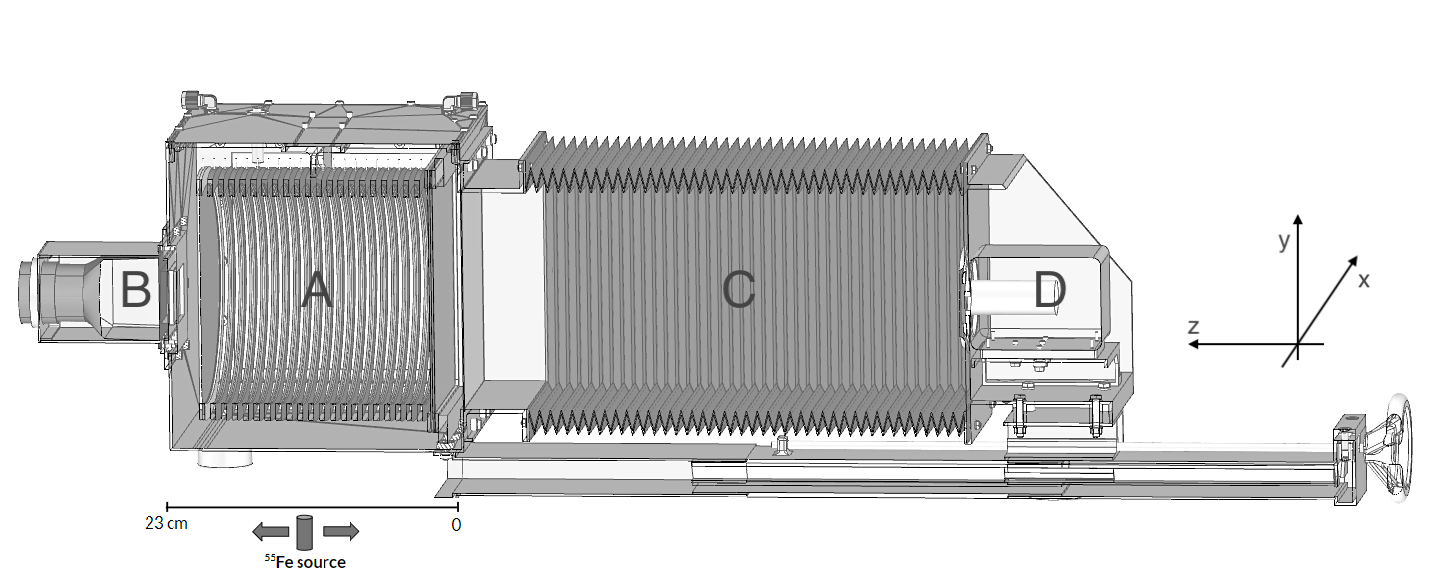
\includegraphics[width=0.85\textwidth]{sex_bw3.png}
\caption{Drawing of the experimental setup. In particular, the elliptical field cage close on one side by the triple-GEM structure and on the other side by the semitransparent cathode (A), the PMT (B), the adaptable bellow (C) and the CMOS camera with its lens (D) are visible. The sliding external $^{55}$Fe source, positioned close to the TPC is also drawn.} \label{fig_lemon_1}
\end{figure}


%In addition to the analysis made in \cite{bib:fe55}, here a cover shield, formed of lead (Pb), was placed surrounding the sensitive volume of the detector (part A in Figure~\ref{fig_lemon_1}), in order to shield it from soft cosmic rays and external natural radioactivity background. And also a simple apparatus was used to enable the modification of the source position along the z axis, which has permitted the study of the detection efficiency as a function of the distance from the GEM planes, that is show in Section~\ref{sec:detectZ}.

%Another important difference is the use of an stronger $^{55}$Fe source, with an activity of about 740 MBq. As the idea was study the effect of the diffusion process a collimator was used to direct the radioactive area of the source.
% Electrons produced within the sensitive volume are drifted by the electric field (Ed) present within the FC, toward the GEMs where the multiplication process takes place.

%The typical operating conditions of the detector are: a drift field Ed = 500 V/cm, an electric field in the GEM produced by VGEM = 460V for each GEM plane and a transfer field Et= 2.5 kV/cm. %The maximum value of (Ed) is limited by the maximum voltage provided by the HV generator (15 kV) used for the measurements reported in this paper.


%\subsection{Data acquisition procedure}
%\label{sec:daqac}

%The experiment trigger decision is based on a fast PMT\footnote{Photonics XP3392, 5 ns rise-time, 76mm square-window} supplied with 1400 V and with transit time around 45ns.
%An image acquiring procedure starts every time the acquisition control system sends a command to the camera making it to start an image capturing process, which lasts for 40 ms (exposure time). During this time a trigger system is activated. It analyzes the PMT current signal and if its current overpasses a certain threshold value, the image is saved for future analysis, as illustrated in Figure~\ref{fig_daq}, otherwise the image is discarded.

%Every time a PMT signal is detected, the camera starts capturing the light produced by the GEM multiplication processes. The camera exposure time was set to 40 ms and during this time the trigger system analyzes the PMT current signal. If its charge overpasses 80 mC, the image is saved for future analysis, as illustrated in Figure~\ref{fig_daq}.


%\begin{figure}[ht]
%\centering
%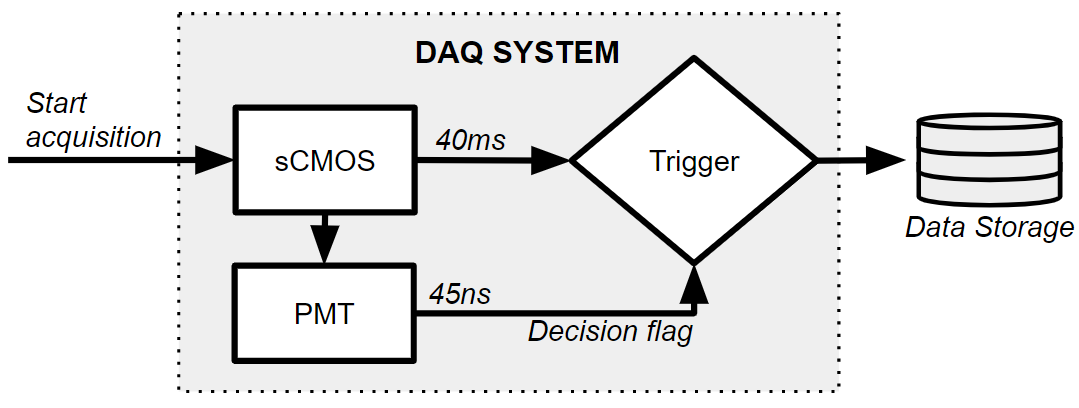
\includegraphics[width=0.6\textwidth]{diagramDaq.PNG}
%\caption{Flowchart of the DAQ process} %\label{fig_daq}
%\end{figure}


\subsection{Acquisition runs}
\label{sec:acrRuns}

Data were acquired using auto-trigger mode. For the proposed study presented in this document, three different acquisition datasets were used, as listed below:

\begin{itemize}
    \item Electronic noise (EN) dataset: produced by lowering down $V\rm _{GEM}$ to a value where the multiplication process is forbidden (6478 images recorded);
    \item Natural radioactivity (NRAD) dataset (composed of cosmic rays and environmental radioactivity): produced by exposing the camera lens and turning on the detector power supplies and raising $V\rm _{GEM}$ to the nominal value of 460 V to allow charge multiplication and secondary light emission during this process (864 images recorded);
    \item Electron Recoils (ER) dataset: the same as the previous item but placing a $^{55}$Fe source near to the detector drift volume (864 images recorded).
    %\item $^{55}$Fe$_{70/30}$ dataset: the same as the previous item but using the $He/CF_4$ -  $70/30$ gas mixture (1000 images recorded).
\end{itemize}


%\subsection{Expected detector's signals}
\subsection{Detector expected signals}

Based on the acquisition datasets defined in section \ref{sec:acrRuns}, particles interacting with the detector gas can have two distinct origins: $^{55}$Fe source and natural radioactivity. The former releases 5.9 keV photons which produce round spots on the image while the latter can be composed of few different particles as photons, electrons and muons. 
Typical signals are shown in  Fig.~\ref{fig_example}:
three interactions of $^{55}$Fe photons in the left top image; two low-energy electrons in the left bottom image; and two high-energy particles and, between them, two interactions of $^{55}$Fe photons in the right image.

%two low-energy electrons on the left; a high-energy electron and a $\rm ^{55}Fe$ spot on the center; and an electron-positron pair and,  between them, two $\rm ^{55}Fe$ spots on the right.
%Muons produce straight tracks as high-energy electrons but usually they cross the whole gas volume.}
%on the left two low-energy electrons are shown; on the center a high-energy electron (muon tracks might be similar to high-energy electrons' but usually muons cross the whole gas volume) and a $\rm ^{55}Fe$ spot can be observed; and, finally, on the right an electron-positron pair production and,  between them, two $\rm ^{55}Fe$ spots can be seen.


\begin{figure}[!ht]
\centering
%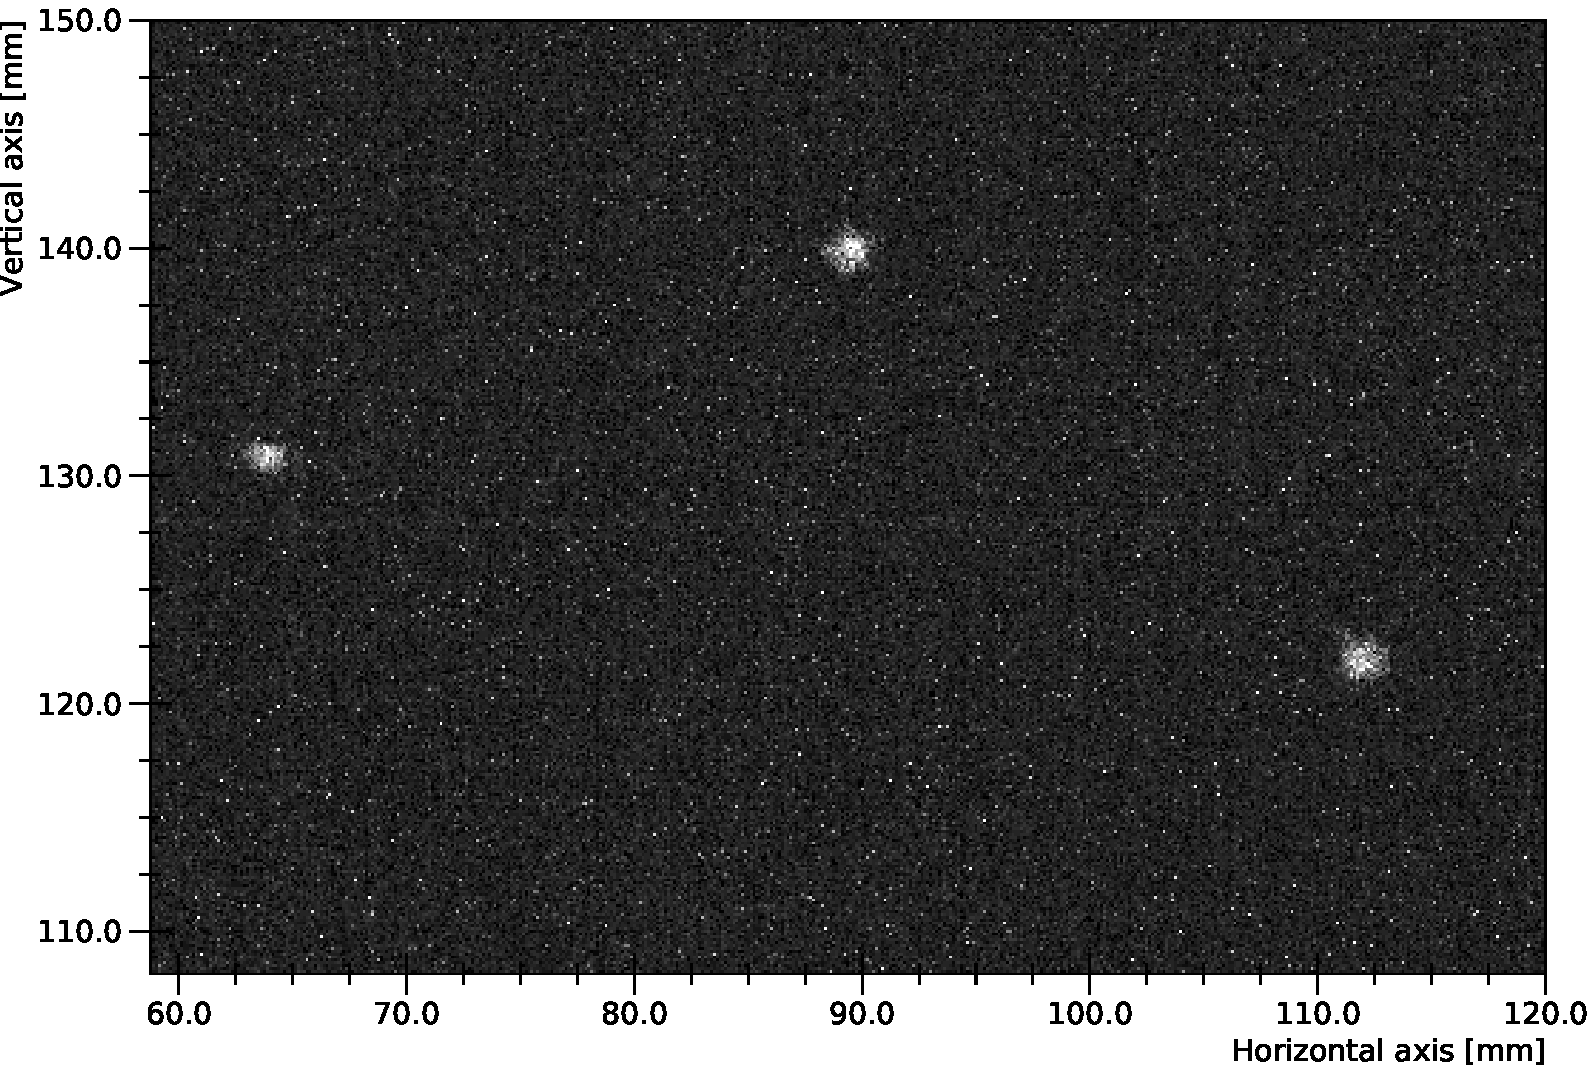
\includegraphics[width=0.445\textwidth]{I31Run2163.pdf}~~~~~~~~
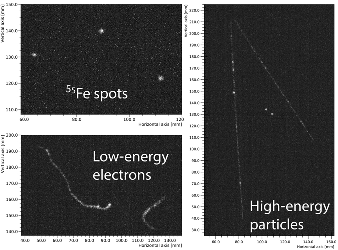
\includegraphics[width=0.7\textwidth]{track_examples.pdf}

%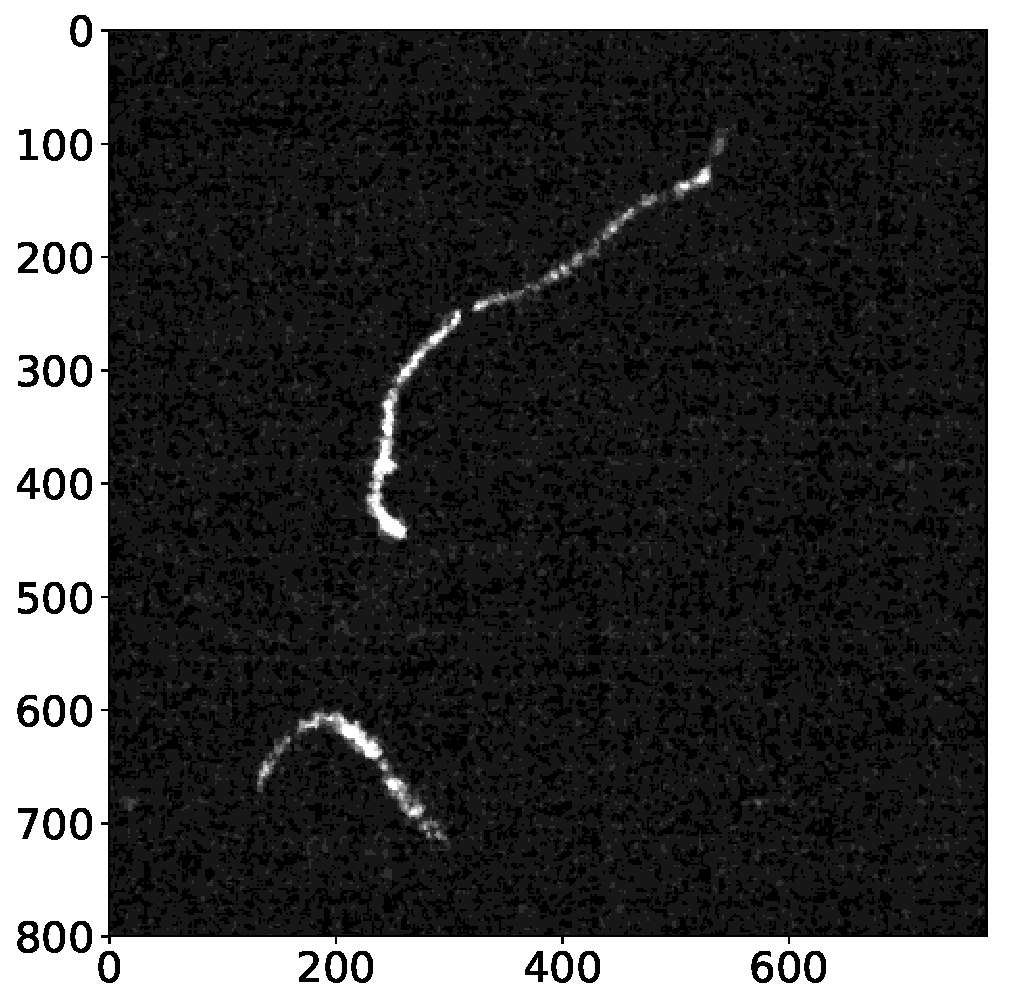
\includegraphics[width=0.257\textwidth]{Ex2163_234zoom1.pdf}
%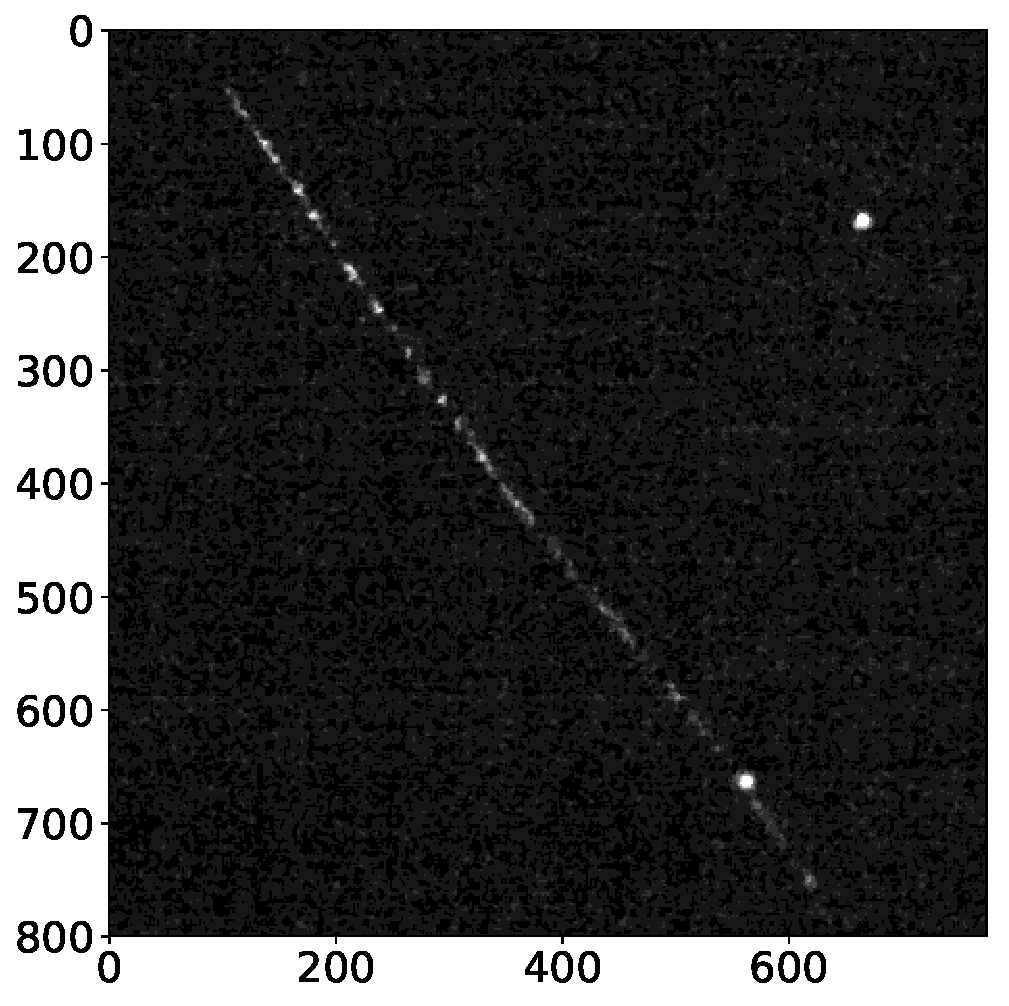
\includegraphics[width=0.257\textwidth]{Ex2163_234zoom2.pdf}
%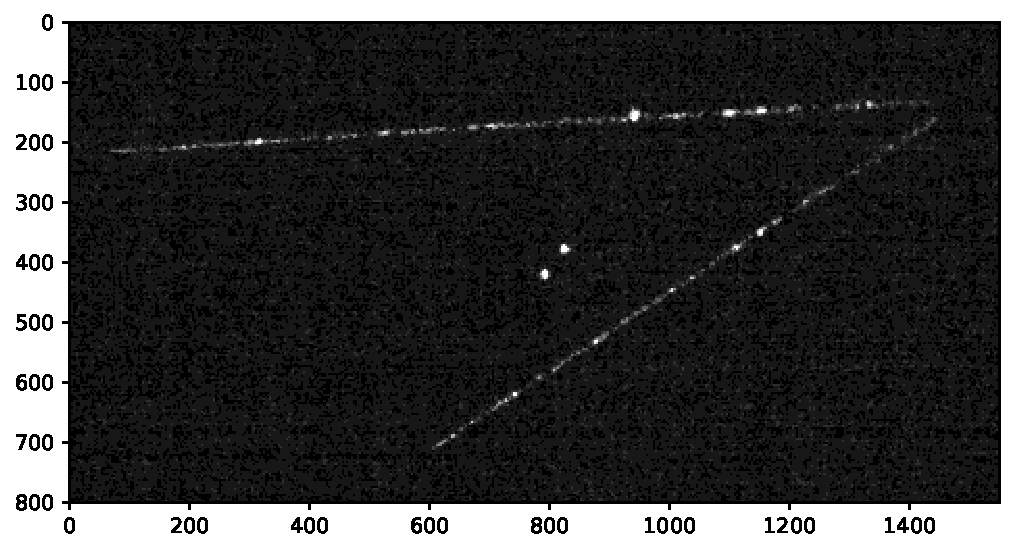
\includegraphics[width=0.474\textwidth]{Ex2163_85zoom.pdf}
%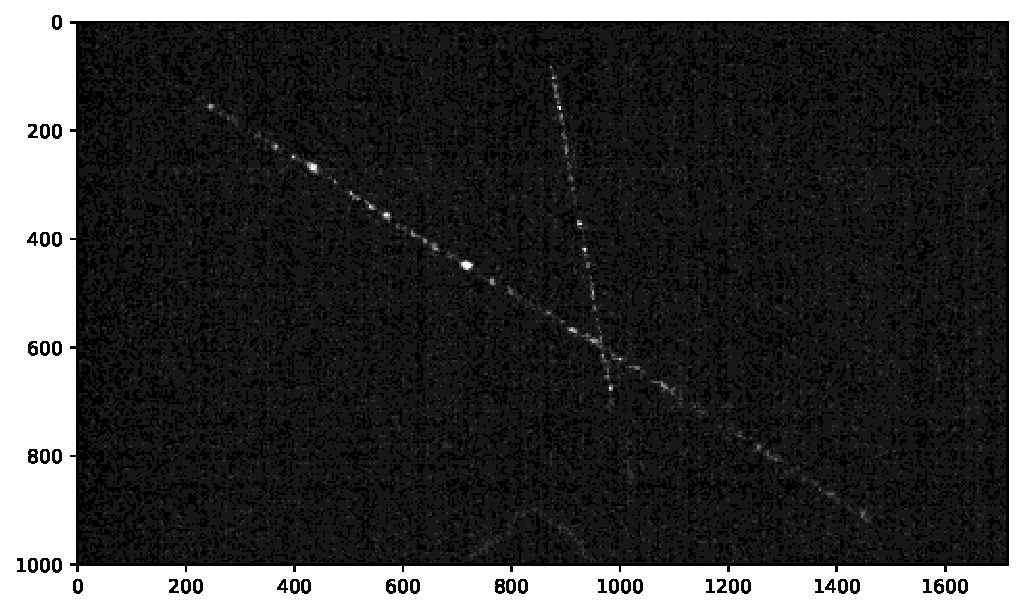
\includegraphics[width=0.55\textwidth]{Ex2163_40zoom.pdf}

\caption{Examples of signals that can occur using the described configuration.} \label{fig_example}
\end{figure}


% \begin{figure}[!ht]
% \centering
% %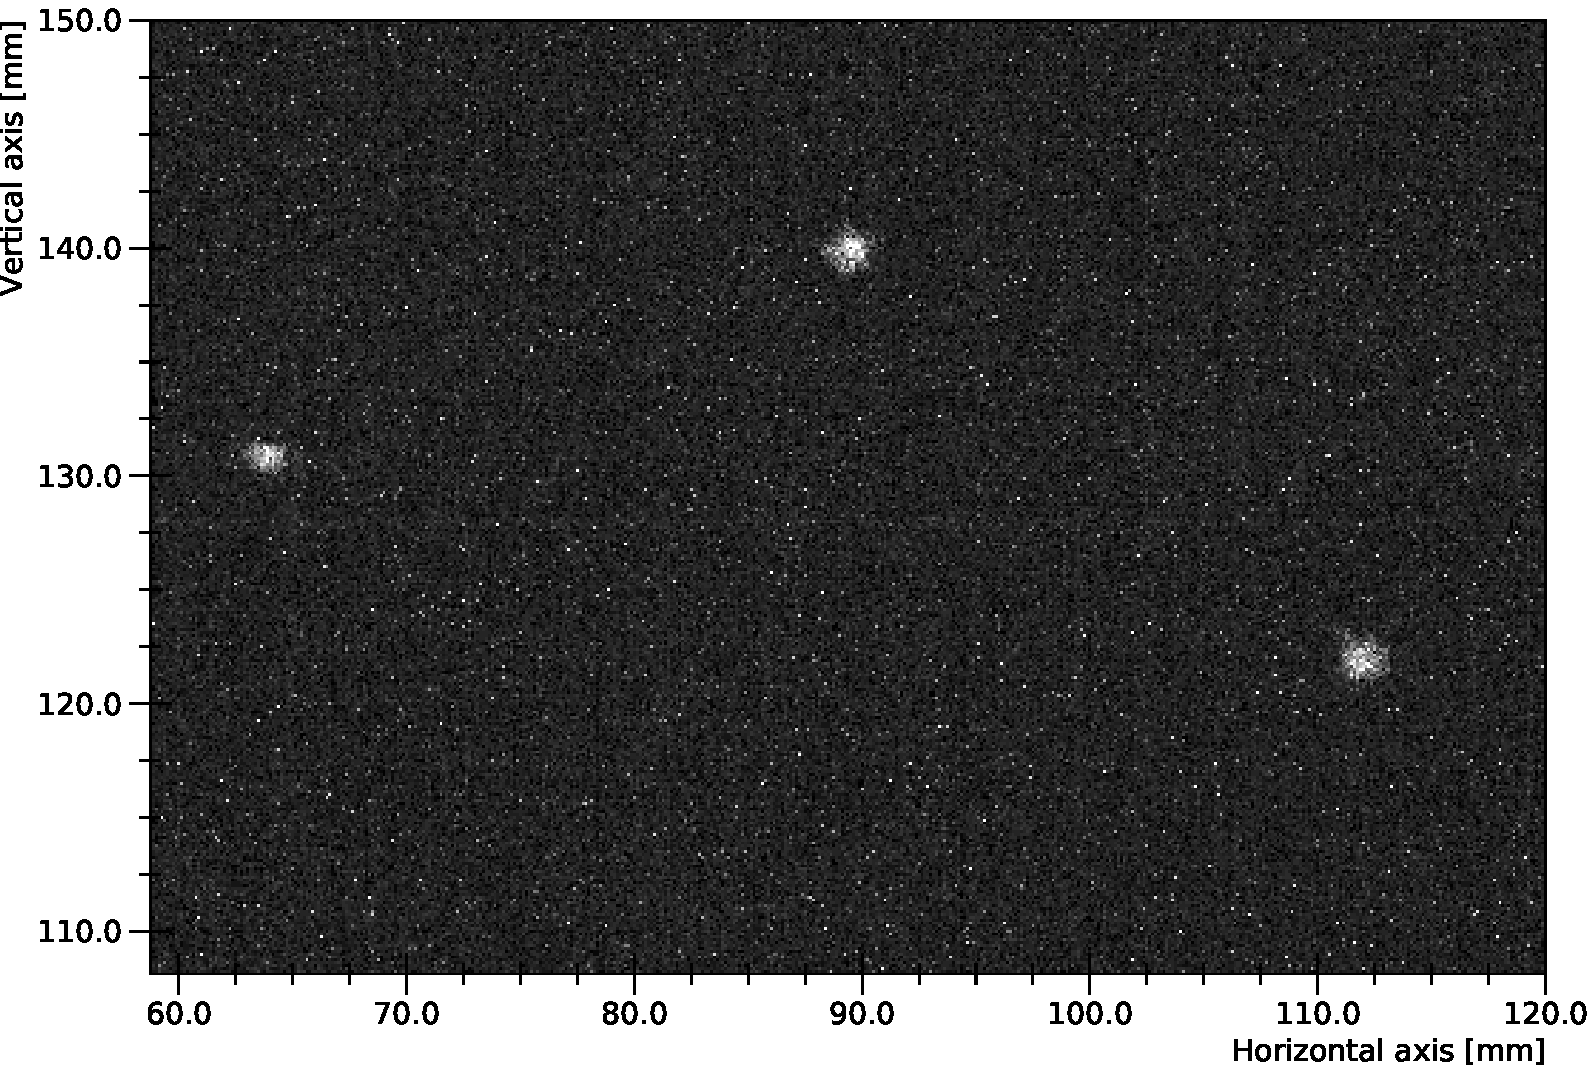
\includegraphics[width=0.445\textwidth]{I31Run2163.pdf}~~~~~~~~
% %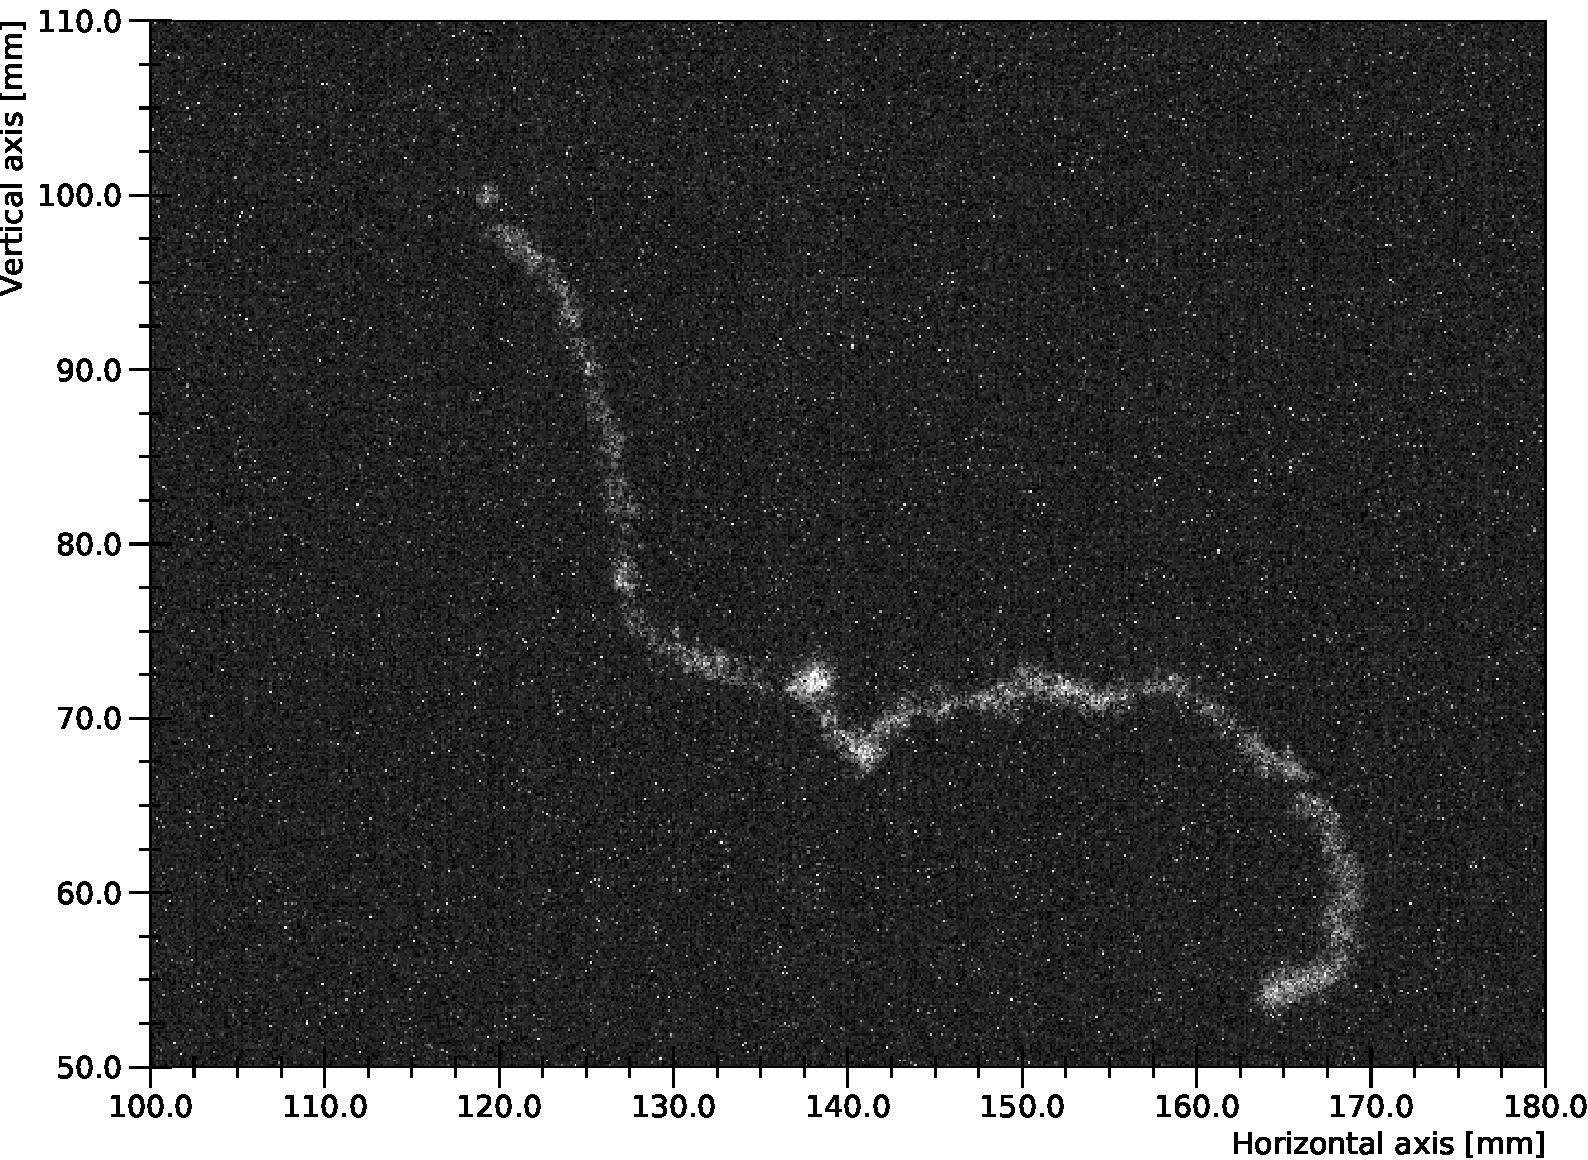
\includegraphics[width=0.41\textwidth]{I32Run2163.pdf}

% 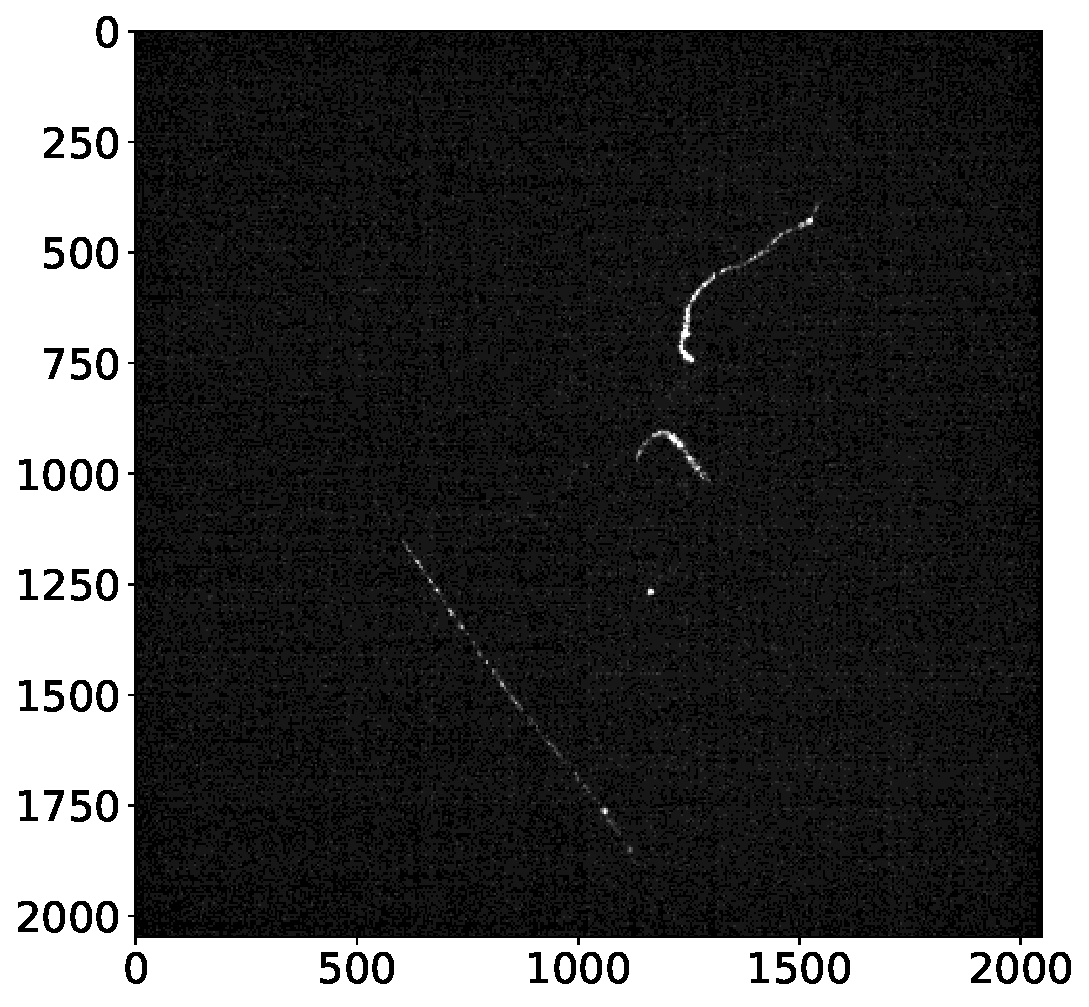
\includegraphics[width=0.49\textwidth]{Ex2163_234.pdf}
% 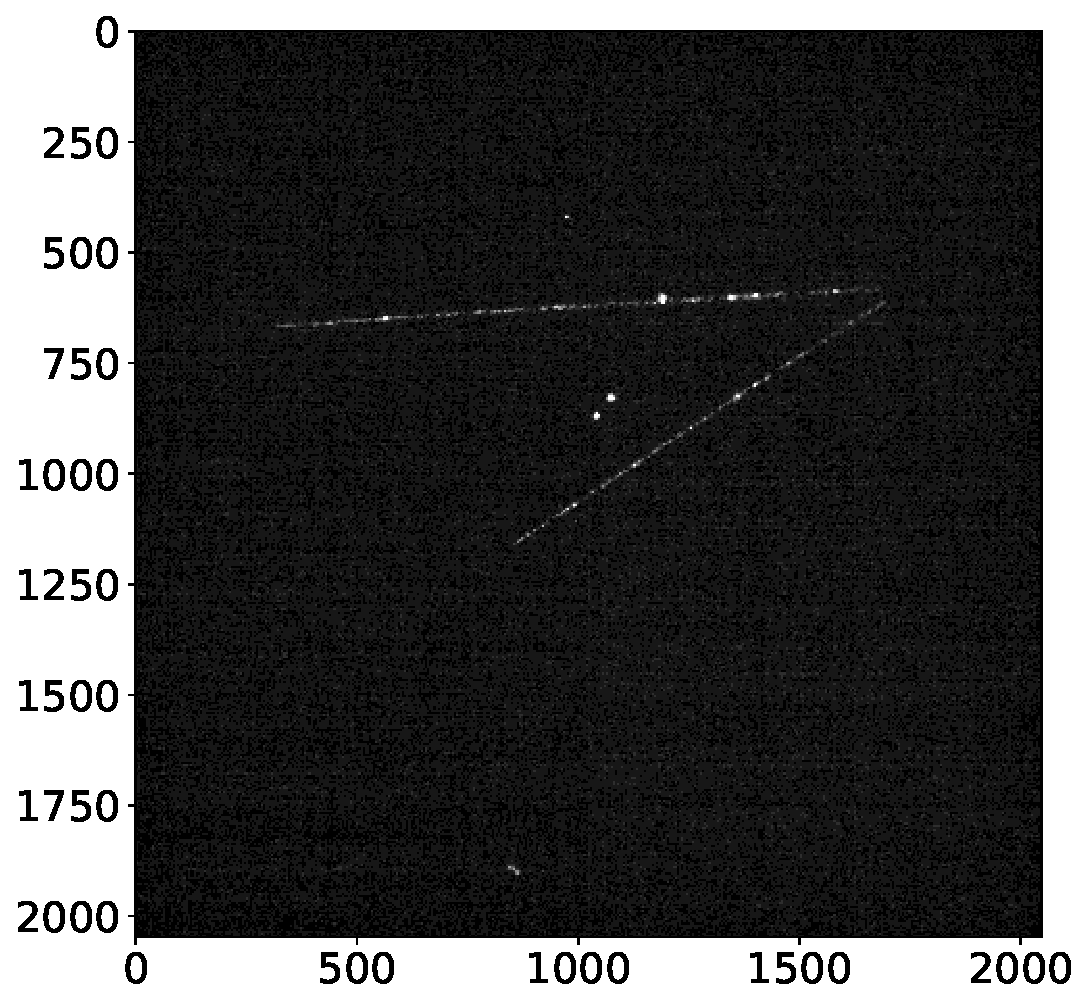
\includegraphics[width=0.49\textwidth]{Ex2163_85.pdf}

% \caption{Examples of signals that can occur using the described configuration.} \label{fig_example}
% \end{figure}


In this work, the signals of interest are those generated by the 5.9 keV photons, which are used to assess the impact of the proposed clustering algorithms on the detector characteristics, focusing mainly on its energy resolution and background-events rejection performance in the energy range of few keV.
%or events-selection performance
%As can be ssuch signals can be clearly distinguisher events-selection performancefrom electronic noise and a good signal-to-noise ratio is expected.
%In relation to background particles, as will be shown, the proposed clustering algorithm is able to efficiently separate signal from background.

\section{Data analysis flow}
\label{sec:daq}

\subsection{Data structure}

The acquisition system provides images with $2048 \times 2048$ pixels captured by the ORCAD Flash CMOS sensor. The photo sensor has an sensitive area of 13312 $\mu m^2$ and each pixel has a size of $6.5 \mu m \times 6.5 \mu m$.
%The camera is equipped with a Schneider lens (D) 325 mm focal length, 0.95 aperture (D).
The camera's exposure time was set to 40 ms and it covers an area of $26 \times 26$ cm$^2$ in relation to the plane of the last layer of the GEM detector. Each pixel provides a response, here called intensity, proportional to the number of collected photons \cite{bib:nim_orange1} added to a baseline, also known as pedestal, which can be defined as the intensity value corresponding to zero photons. Specifically, the pedestal average value of the sensor is about 99 counts, however it can vary from pixel to pixel.
Additionally, the noise level is another important parameter that can vary from pixel to pixel.
Those effects can be seen in Fig. \ref{fig:sensor_noise} which shows the mean and standard deviation distributions of the noise as computed for each pixel, produced with the EN dataset.
To account for such variations, both the pixel baseline ($\mu_i$) and its average noise ($\sigma_i$), calculated as the standard deviation of the pedestal distribution,  are estimated for every single pixel $i$ before running the event reconstruction procedure.


%using an electronic-noise dataset (as defined in section \ref{sec:acrRuns}).

\begin{figure}[ht]
\centering
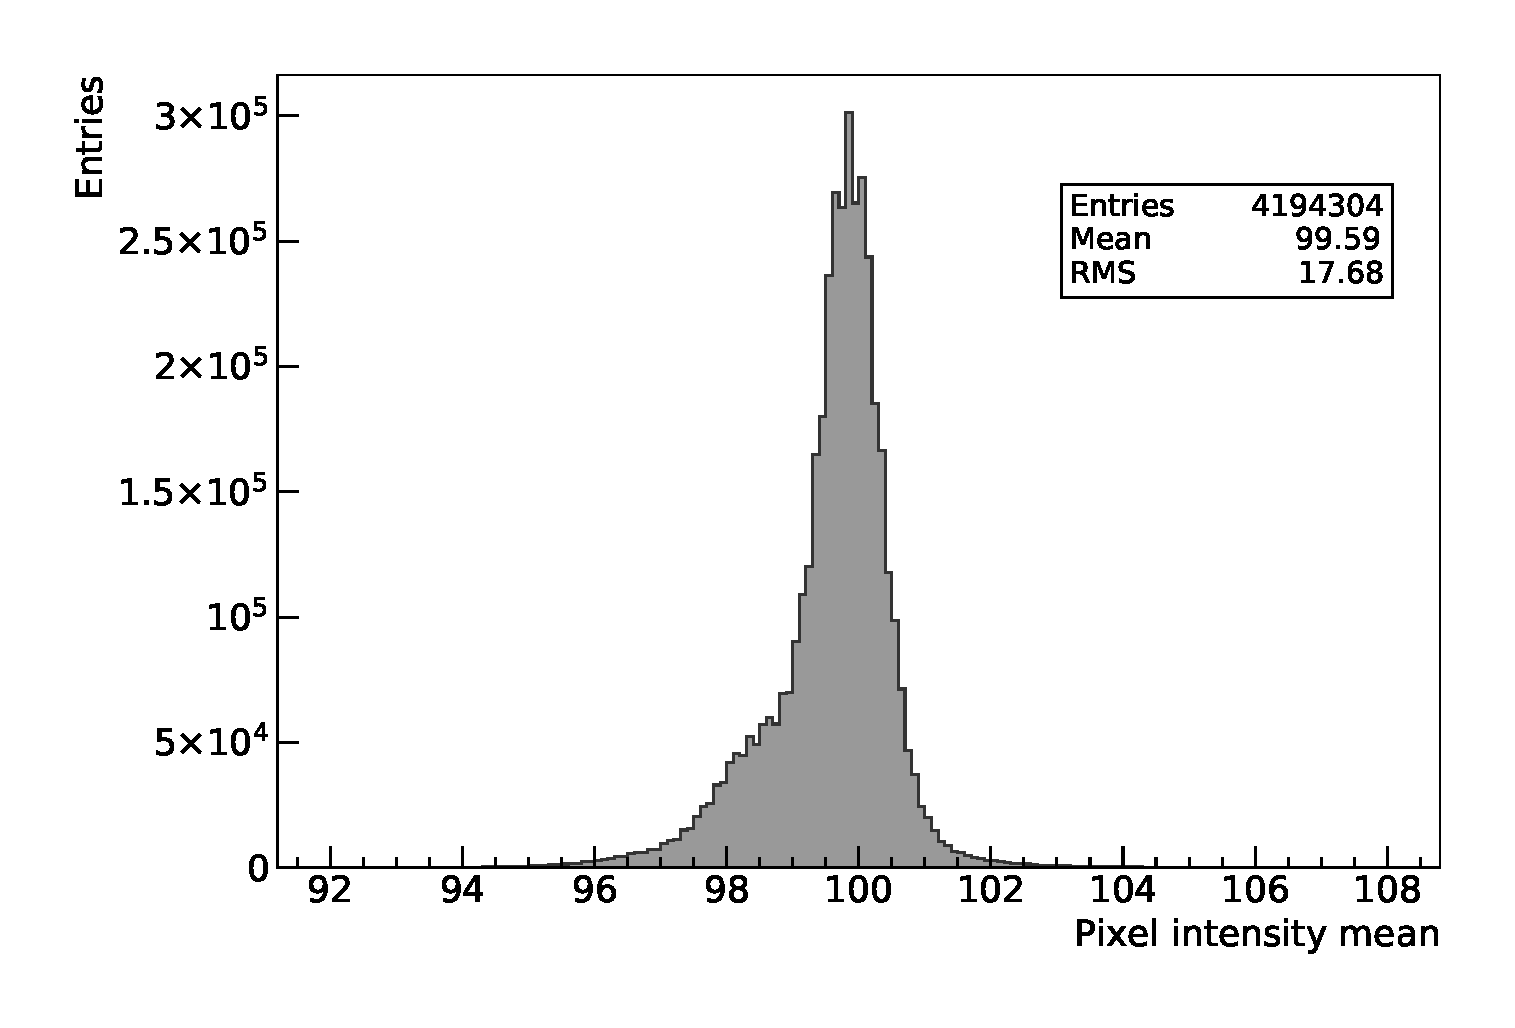
\includegraphics[width=0.45\textwidth]{Mean_2155.pdf}
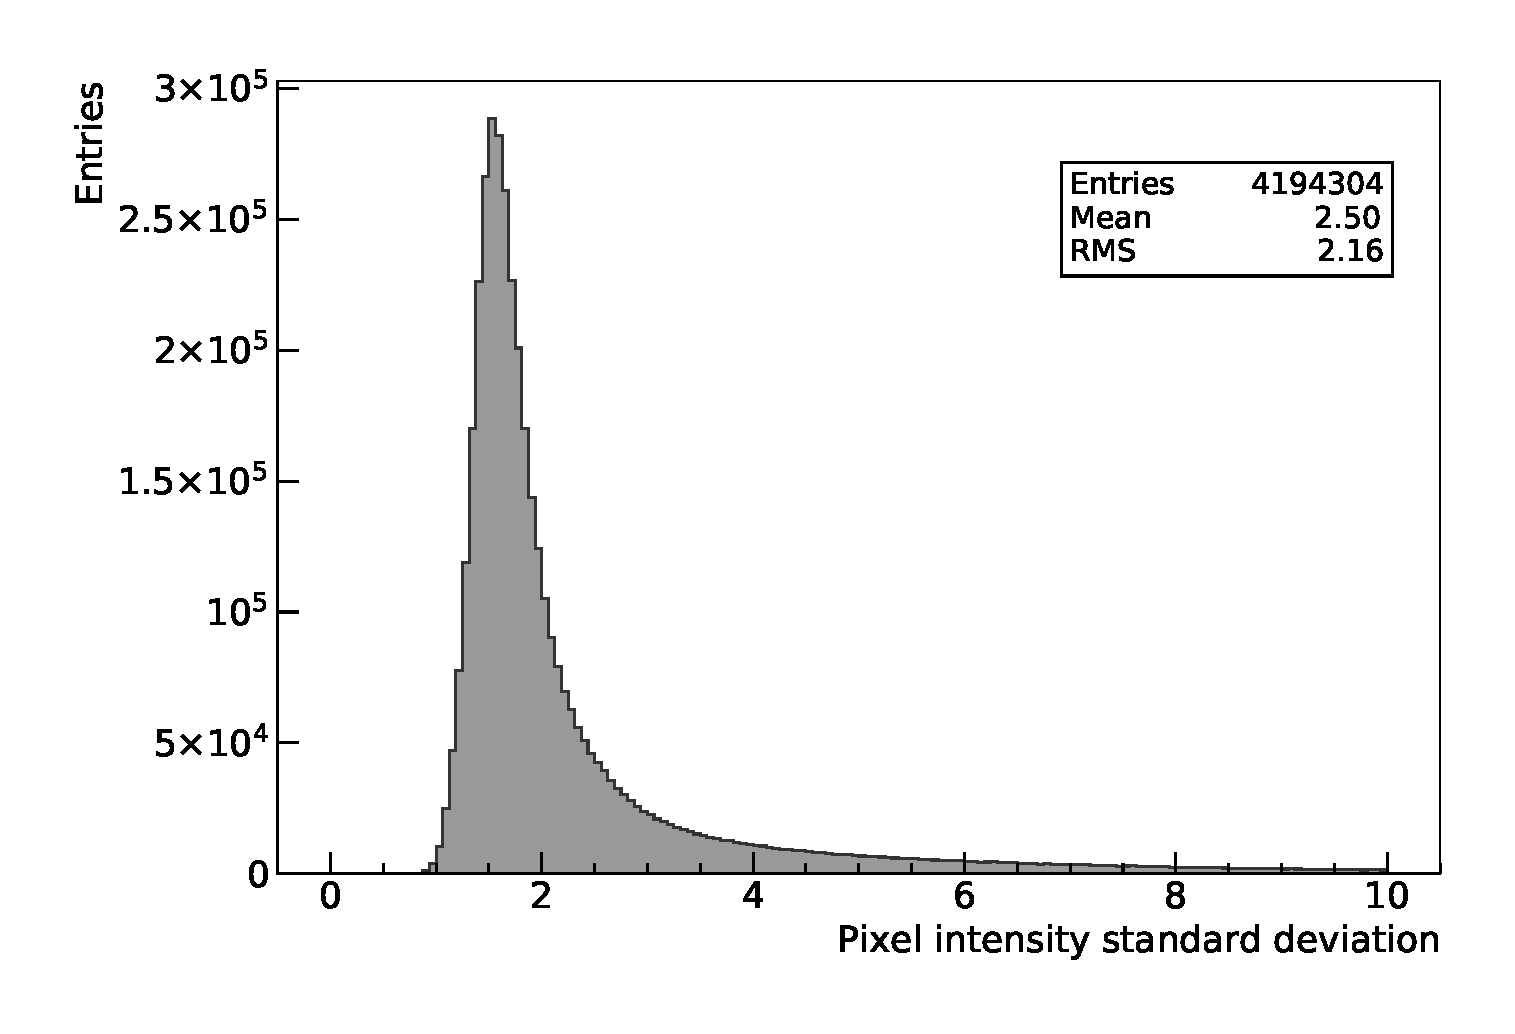
\includegraphics[width=0.45\textwidth]{Std_2155.pdf}
\caption{Mean and standard deviation distributions of the sensor's pixels noise.}
\label{fig:sensor_noise}
\end{figure}






\subsection{Overview of the event reconstruction procedure}

The current CYGNO's event-reconstruction algorithm is represented in the flowchart shown in Fig.~\ref{fig_algo} and it is described below.

\begin{figure}[ht]
\centering
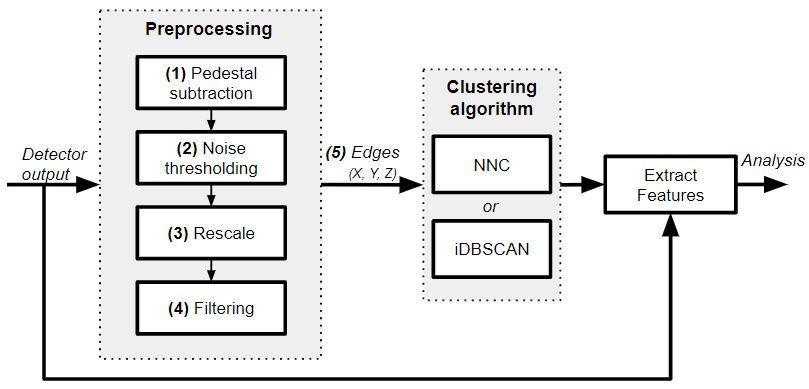
\includegraphics[width=0.7\textwidth]{fluxgram_algorithm.PNG}
\caption{Flowchart of the CYGNO's event-reconstruction algorithm.}
\label{fig_algo}
\end{figure}


\begin{enumerate}
\addtocounter{enumi}{0}
    
    \item Pedestal subtraction is carried out pixel by pixel by subtracting $\mu_i$ from their original intensity values, generating new intensity values defined as $I_i$. 

    \item Lower and upper thresholds are applied to $I_i$.
    While the upper limit is set to $100$ counts, the lower limit is set to 1.3 times $\sigma_i$.
    The upper limit allows to remove pixels with a too large intensity, very likely not due to ionization in gas, while the lower limit was optimized and set to be just above noise level to ensure a good detection efficiency, but not too low in order not to overload the event-reconstruction algorithm with pixels dominated by noise. Pixels outside those limits have their intensities reset to zero.
    
    
    \item Images are then rescaled to $512 \times 512$ pixels, for CPU reasons, so that each $4 \times 4$ matrix, called macro-pixel, is assigned an intensity value corresponding to the average of the intensities $I_i$ of the 16 pixels occupying the same area of the sensor. %over the $2048 \times 2048$ image.
    %this process is done by get the mean value of 16 pixels (4x4) on the full resolution image to represent them on the rescaled image.
    
    \item The rescaled image goes then through a filtering stage based on a $4 \times 4$ median filter that replaces a given macro-pixel intensity by the median of all macro-pixels in its neighborhood $w$, as given by Equation \ref{eq10} \cite{filterStudy}, where $f(x,y)$ is the intensity of the macro-pixel $(x,y)$.
    
     \begin{equation}
             g(x,y) = median\{f(x,y), (x,y) \in w\}
             \label{eq10}
         \end{equation}
        
    Such filter is widely used in many applications due to its effective noise suppression capability and high computational efficiency~\cite{Dong_2007}.
    Tests performed on the EN dataset (see section \ref{sec:acrRuns}) showed that this filter is able to reduce the number of noise pixels sent to the clustering algorithm by a factor of 3.07 $\pm$ 0.02.
    
    
        
        
  
    
    \item Finally, the coordinates (X, Y) and respective intensities (Z) of the pixels with non-zero $I_i$ values are sent to the clustering algorithm whose output is used to extract clusters' features such as integrated light, length and width, computed over the full-resolution image. Those features are then used to select events of interest. 
\end{enumerate}

In this work three features, extracted from the clusters, are used: 
\begin{itemize}
    %\item Length and width: each cluster has its eigenvalues \cite{jolliffe2002springer} computed and used as a measure of length (highest eigenvalue) and width (lowest eigenvalue). 
    %\textcolor{purple}{not very clear}
    
    \item Length and width:
    the full length of the major and minor axes along the two eigenvectors of the (X,Y) pixel matrix in the context of Principal Component Analysis \cite{jolliffe2002springer} are assigned as the length and width of the cluster, respectively.
    %each cluster forms a set of data-points distributed on a Cartesian plane that can be used to calculate the variance of its two principal components in the context of Principal Component Analysis \cite{jolliffe2002springer}.
    %The major variance value is used as a measure of the cluster's length while the minor one is used as a measure of its width.
    

    %first, the covariance matrix is calculated between the X and Y coordinates, using this information the eigenvalues and eigenvectors can be calculated. Then,it is possible to rotate the clusters to the abscissa axis. After rotating the smallest values in X and Y are calculated and subtracted from the respective coordinate, making the beginning of the cluster the coordinate (0.0). Finally, a 2D histogram is created in order to obtain the X and Y projections and perform the RMS calculation on each axis. These RMS' represents the length (major axis) and width (minor axis) features.
    
    \item Cluster light: calculated as the sum of all the pixel $I_i$ intensities belonging to the cluster.
\end{itemize}

%\textcolor{blue}{ The upper limit is justified by the fact that particle tracks are not likely to produce pixels with intensity above 200 counts while the lower limit is set to be just above noise level but not so low as to overload the event-reconstruction algorithm.}





%The resulting images are sent to a clustering algorithm and its output is used to extract clusters' features such as integrated light, length and width, computed over the full-resolution image. Finally, those features are used to select events of interest.



%: electronic recoils from 5.9 keV photons interacting in the gas for this work.

%sion , after data a preprocessing phase is carried on with a re-scale of the image ($512x512$), a pedestal subtraction are made, the pedestal ($p$) of each pixel is evaluated as the average number of counts recorded in the run ($m$) and the standard deviation ($s$), and it is subtracted to each image as $p=m+s$, then a $4x4$ Median Filter~\cite{tukey1977exploratory} is applied as denoise tool and at the end also an upper threshold is set as $200$ counts. After, the coordinates of the remained pixels are used as an input for the clustering algorithm (Near Neighbour Clustering or an iterative DBSCAN). At last, the output of the clustering algorithm is used to extract some features (e.g. cluster light, length and width) of each cluster using the full size image.

%\begin{figure}[ht]
%\centering
%    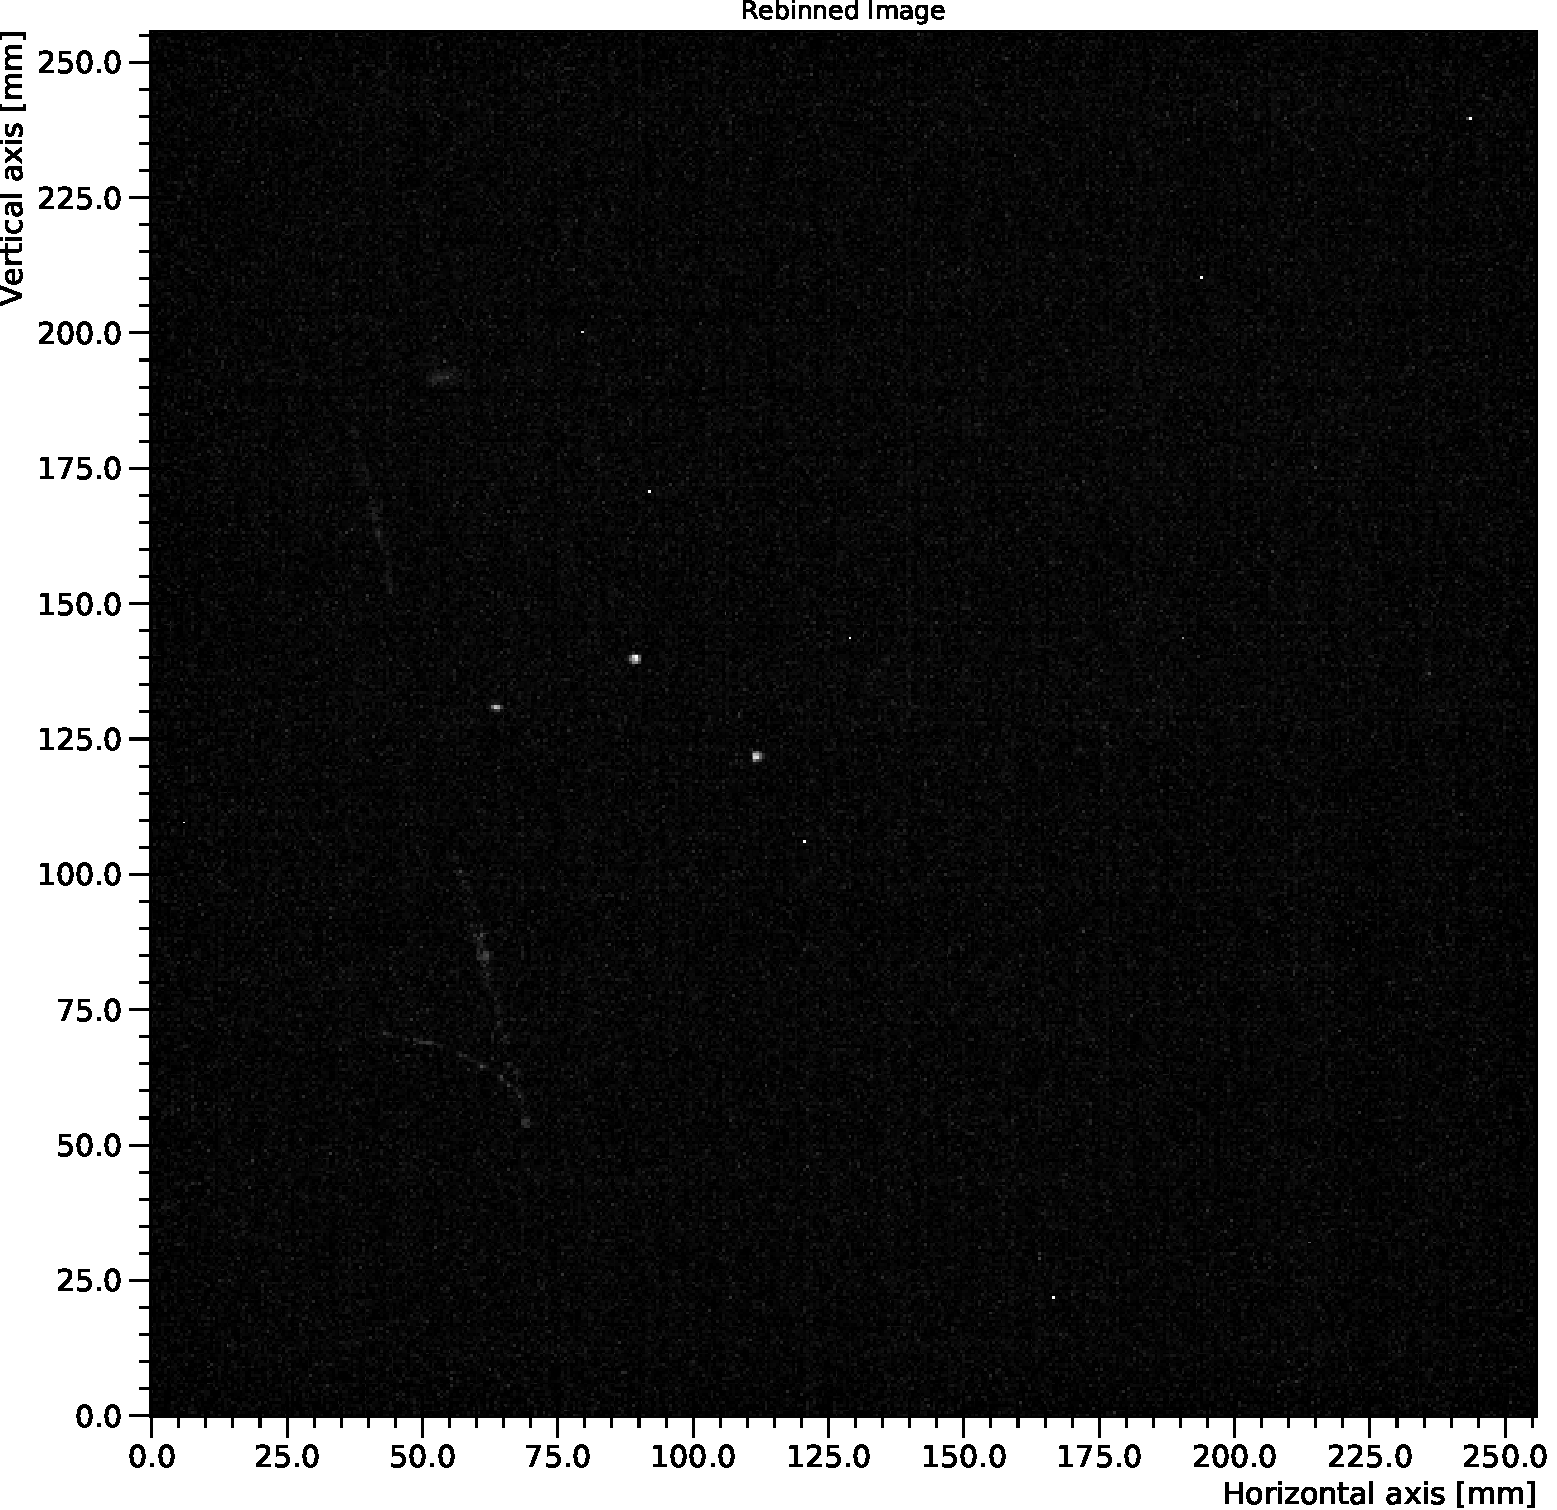
\includegraphics[width=0.45\textwidth]{pic_run02163_ev31_rebinIma.pdf}
%    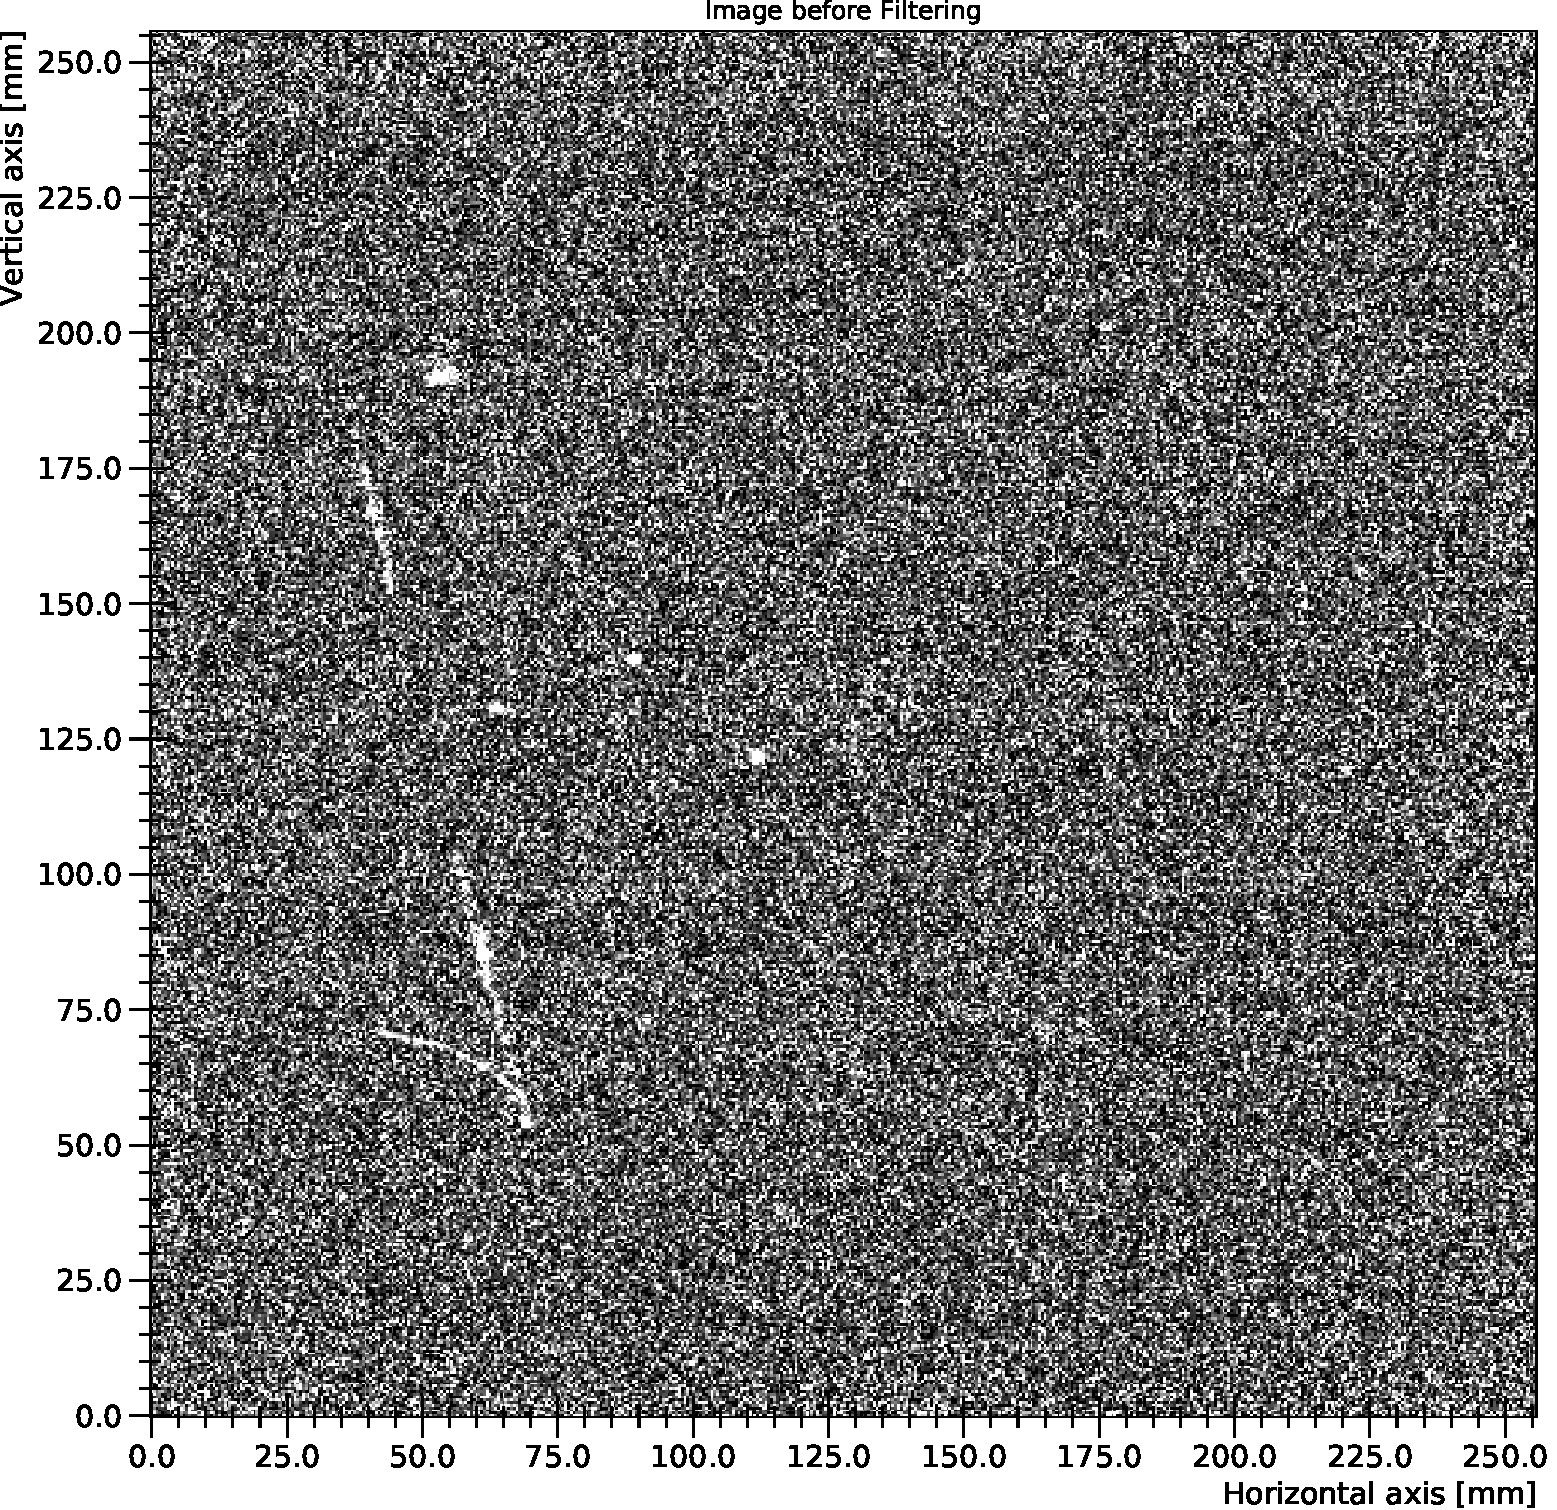
\includegraphics[width=0.45\textwidth]{pic_run02163_ev31_edgesWoIma.pdf}
%    \\
%    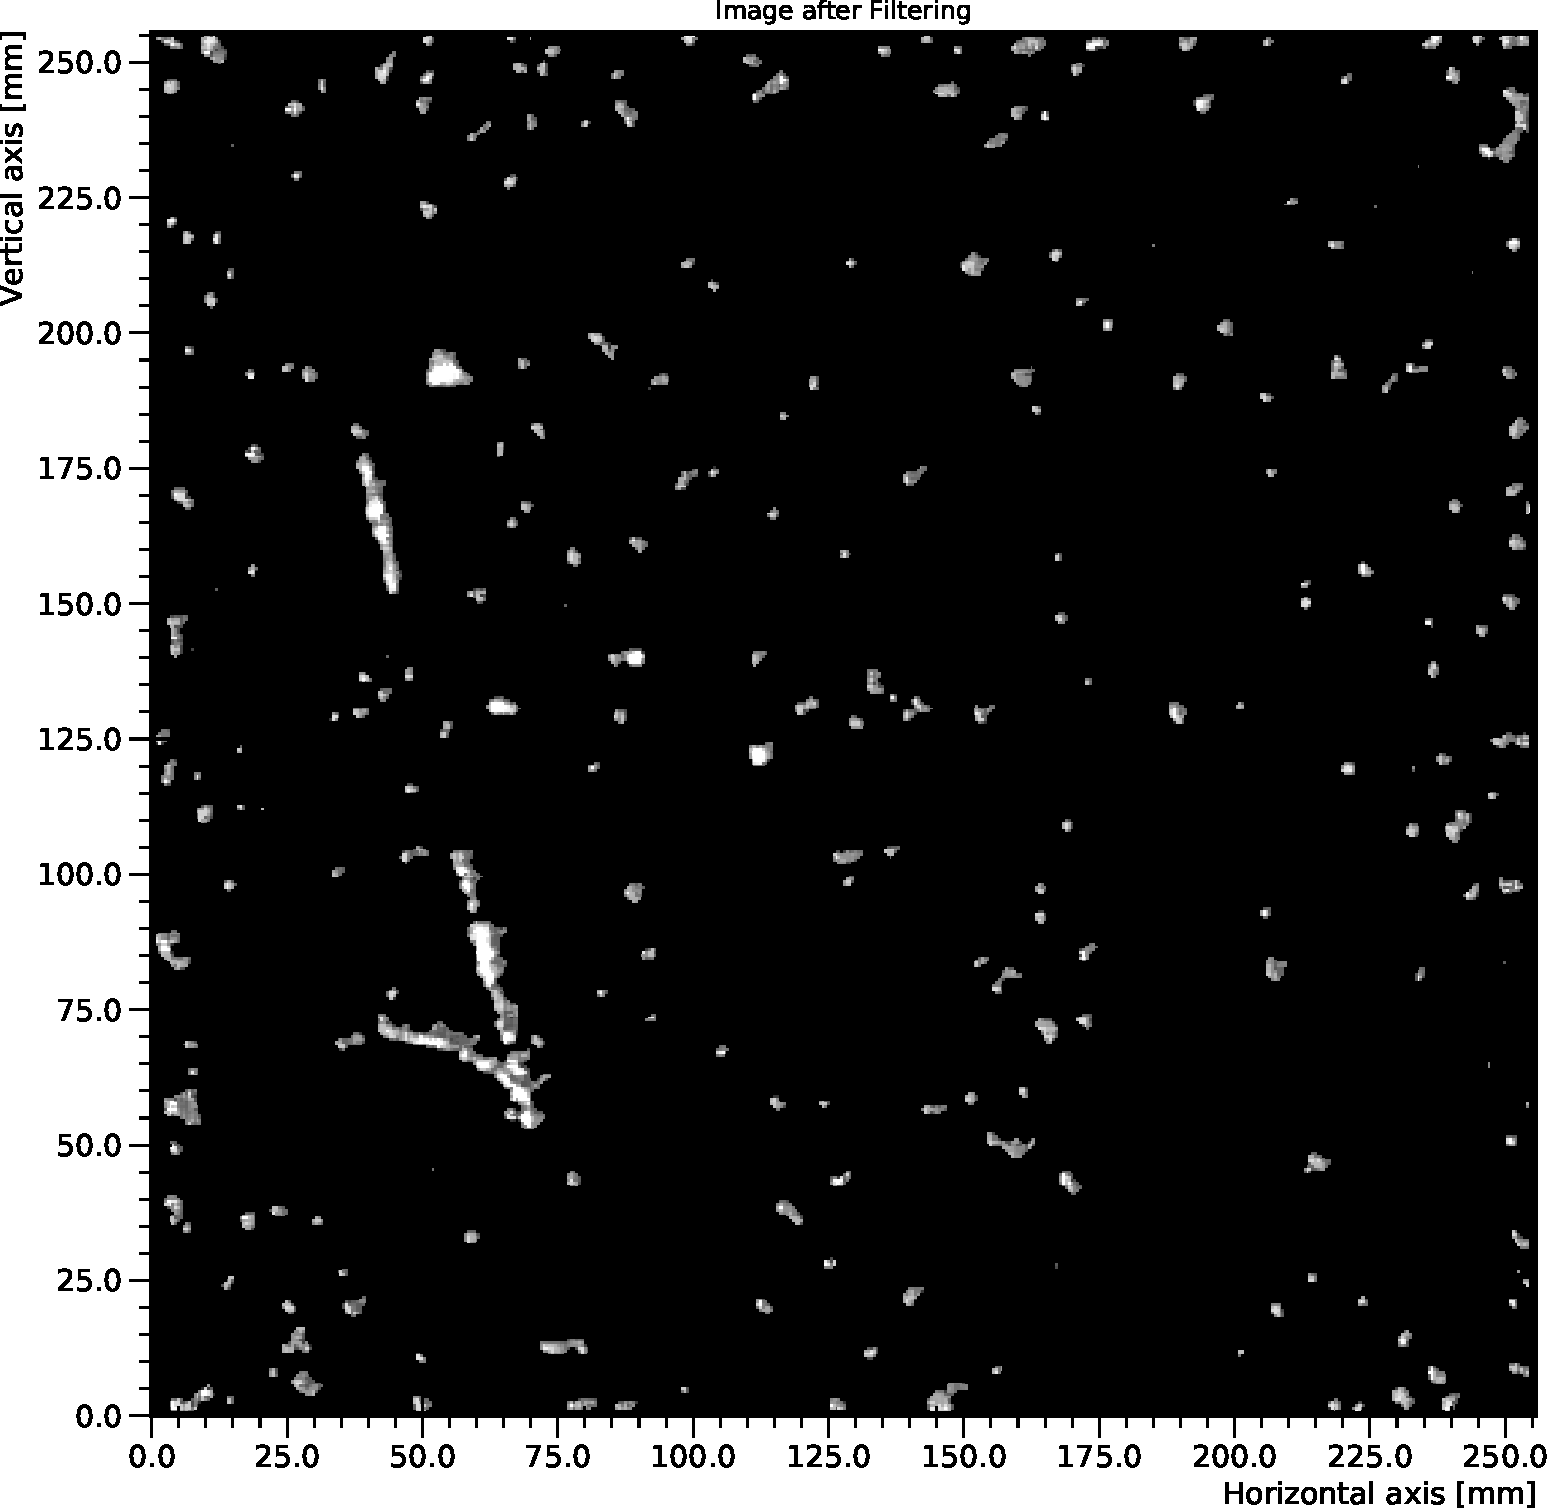
\includegraphics[width=0.45\textwidth]{pic_run02163_ev31_edgesIma.pdf}
%    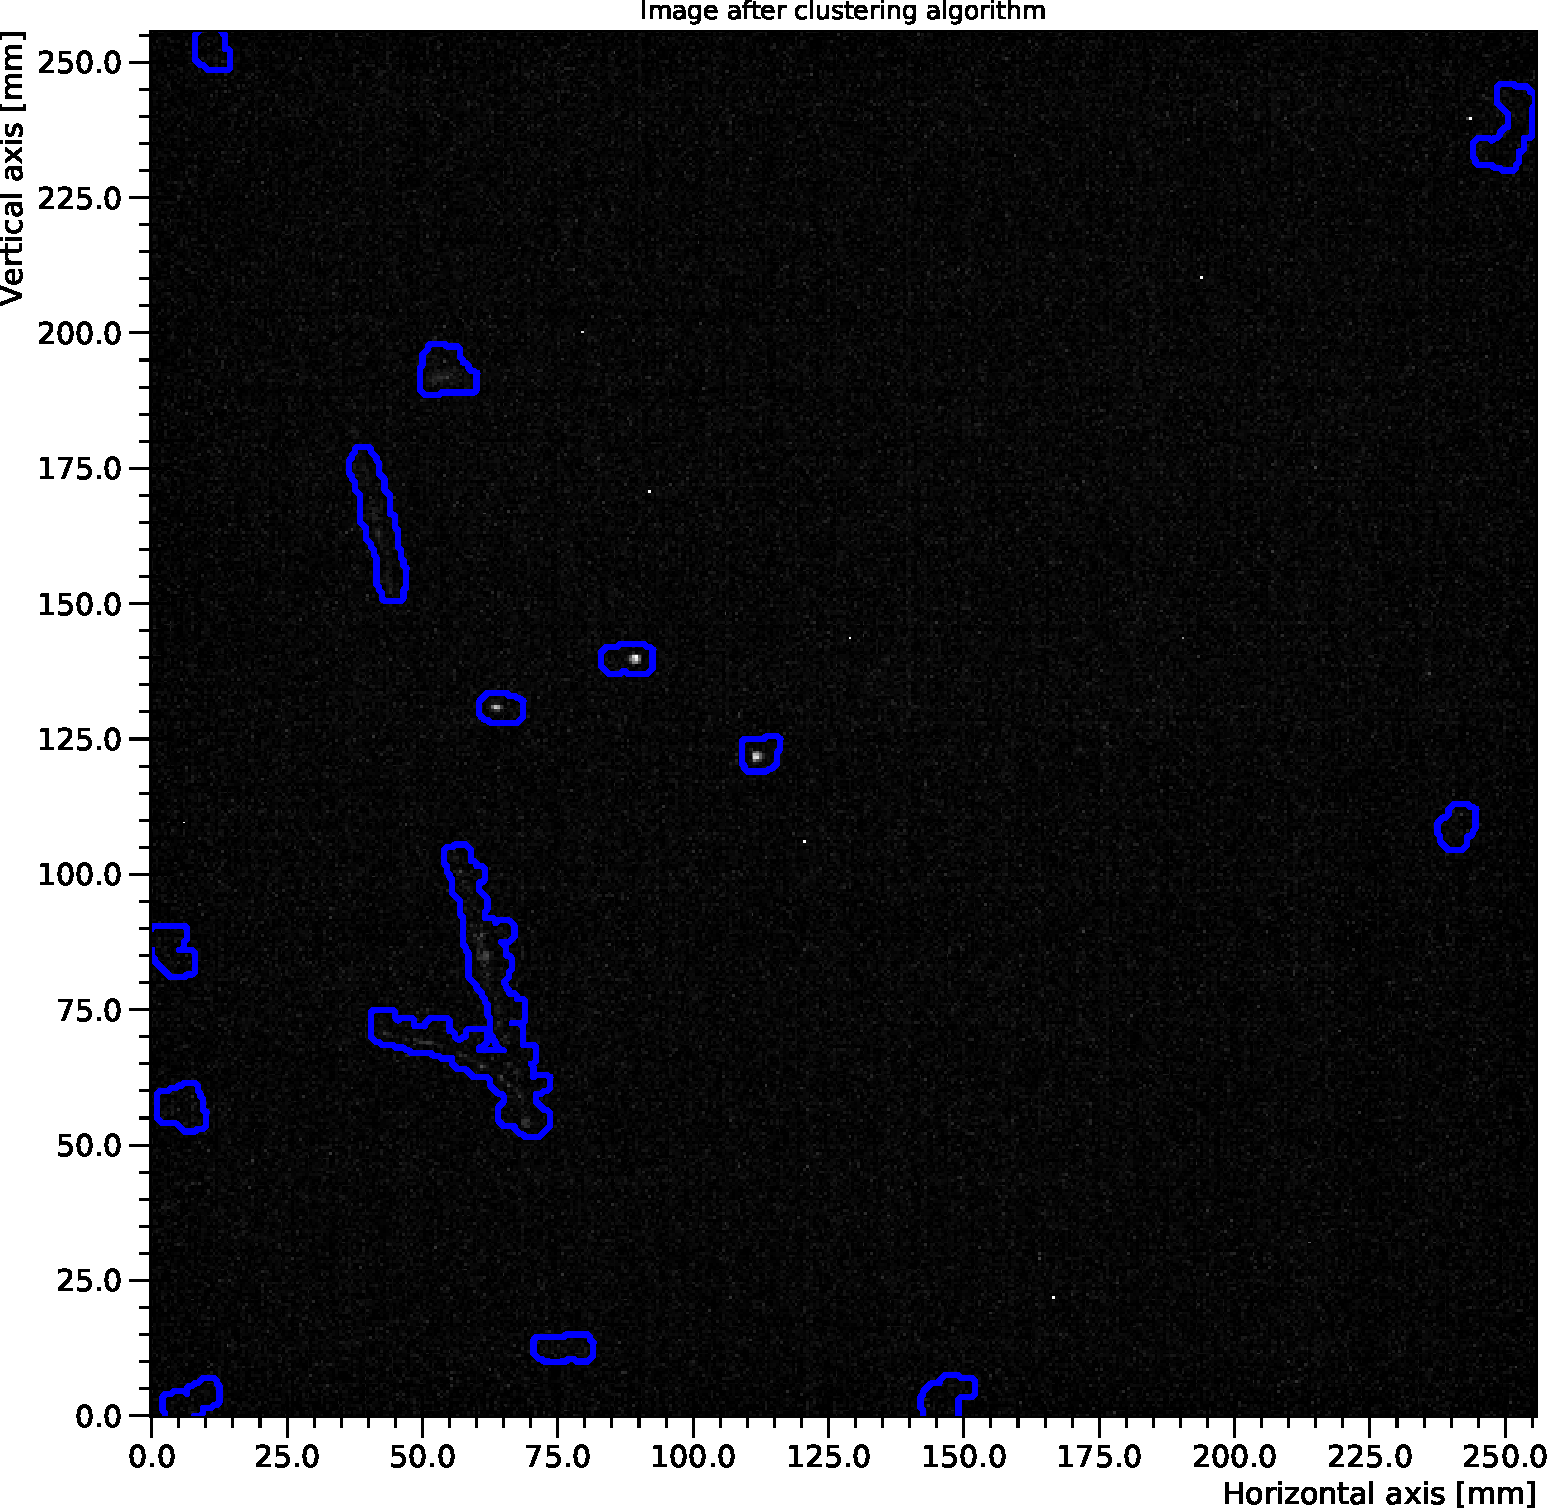
\includegraphics[width=0.45\textwidth]{pic_run02163_ev31_2nd_3D.pdf}
%    \caption{Flowchart of the reconstruction algorithm.}
%\label{fig_process}
%\end{figure}



As mentioned before, prior to iDBSCAN, the CYGNO clustering algorithm was based on the widely employed NNC method. Basically it groups neighboring pixels that went through a selection similar to the one in step 3. A detector performance study using such method was presented in \cite{bib:fe55}.
%Recently, a new clustering procedure called intensity-based DBSCAN (iDBSCAN) was implemented and included as part of the Experiment's official event-reconstruction algorithm.
%Since then, a new clustering procedure has been implemented, named intensity-based DBSCAN (iDBSCAN), and is currently in use by the Experiment.
%This section will be used to describe iDBSCAN and to validate its parameters values. As will be shown in section \ref{sec:algoComp}, iDBSCAN was able to produce an improvement of the CYGNO's clustering stage, regarding the low-energy region of the
%detector, for electron recoil events produced by 5.9 keV photons.
%the few keV energy region of the detector.
%could help to improve some of the characteristics of the LEMON detector. 

\subsection{The CYGNO intensity-based clustering algorithm}
\label{sec:dbscan}


\subsubsection{iDBSCAN}
%The density-based clustering algorithm, known as DBSCAN \cite{dbscan1996}, is capable of searching for sets of signals that present the same characteristics and arbitrary shapes. It requires only the configuration of two parameters: \textit{eps} and \textit{minpoints}, that represent the search radius by neighbors and the number of neighbors within that radius to be considered a cluster, respectively.

%As depicted in the Introduction section, CYGNO Experiment currently uses the density-based algorithm known as DBSCAN \cite{dbscan1996} as a basis for its clustering stage.
As in many areas, in particle physics it is possible to insert a priori knowledge about the detection system and its data to improve the performance of the clustering task \cite{wagstaff2000clustering}. In this sense, a modification of DBSCAN \cite{scikit-learn} clustering algorithm was implemented, to better match the experimental conditions and data of the LEMOn detector.
As mentioned before, DBSCAN has only two parameters: $\epsilon$ and $N_{min}$. Whenever the number of neighboring elements inside a hyper-sphere reaches the $N_{min}$ value, the center element and all its neighbors are activated to start the formation of a cluster.
Then, the same process happens to all the neighboring elements in order to expand the starting cluster, to form a final cluster. This process is repeated to all the data elements.
To be applied to CYGNO, instead of using the number of elements as a parameter to decide if the elements inside a hyper-sphere make part of a cluster, the sum of their intensity values is used. Consequently, the $N_{min}$ become a parameter related to the total intensity within a hyper-sphere instead of to the number of elements.
Therefore, rather than having each pixel counted as a unit when computing the number of pixels inside a given hyper-sphere, each pixel counts $I_i$ times.
If the total intensity is equal or greater than a certain value ($N_{min}$), they are considered as making part of a cluster.


%This new method works by performing iterations of the naive algorithm; in other words, the parameters are configured to look for a particular type of signal in each iteration and simulating the $3^{rd}$ dimension (the intensity); which means to use the coordinate of the pixel (x,y) that passed through the threshold and replicate its coordinate by intensity (z). In this way, it is possible to emulate the third dimension (photons) without have to lead with the curse of dimensionality~\cite{porter2013statistical}.


%\subsection{Validation of the clustering parameters}

\subsubsection{Validation of the iDBSCAN parameters}

The CYGNO Collaboration is currently using iDBSCAN for the clustering method in its event-reconstruction. The iDBSCAN performance for signals produced by the interactions of photons from $^{55}$Fe has been studied as a function of different values of the its parameters: $\epsilon$ and $N_{min}$.
%For studies related to the low energy region, as for the $^{55}$Fe photons, CYGNO has been using iDBSCAN configured with the following parameters values: 5.8 for \textit{eps} and 30 for \textit{minpoints}.
In order to evaluate those values, a test on the detector efficiency and background rejection was carried out: a scan over the two iDBSCAN parameters has been performed.
%In order to test the efficiency of CYGNO's DBSCAN in finding $^{55}$Fe spots, a scan over its two parameters has been performed.
While the $\epsilon$ ($N_{min}$) parameter will be fixed to a value of 5.8 (30), the other parameter's value will be swept from 5 to 50 (4 to 10). 
Figure \ref{fig:epsscan} (left) shows the total number of clusters found as a function of $\epsilon$ for two distinct datasets: ER and NRAD.
%The former contains low energy electrons recoils and natural radioactive events and the latter only natural radioactive events.
For low $\epsilon$ values the number of NRAD clusters tends to increase, indicating an increase of background contamination. However, for $\epsilon$ values between 5 and 7, this contamination rate stabilizes around a minimum value.
Figure~\ref{fig:epsscan} (right) shows the same trend, while counting only clusters with an integral in the range 2000–4000 photons, characteristic of $^{55}$Fe deposits. This region refers to the energy region of the $^{55}$Fe produced electron recoils (see Fig.~\ref{fig_compfe}).

\begin{figure}[ht]
\centering
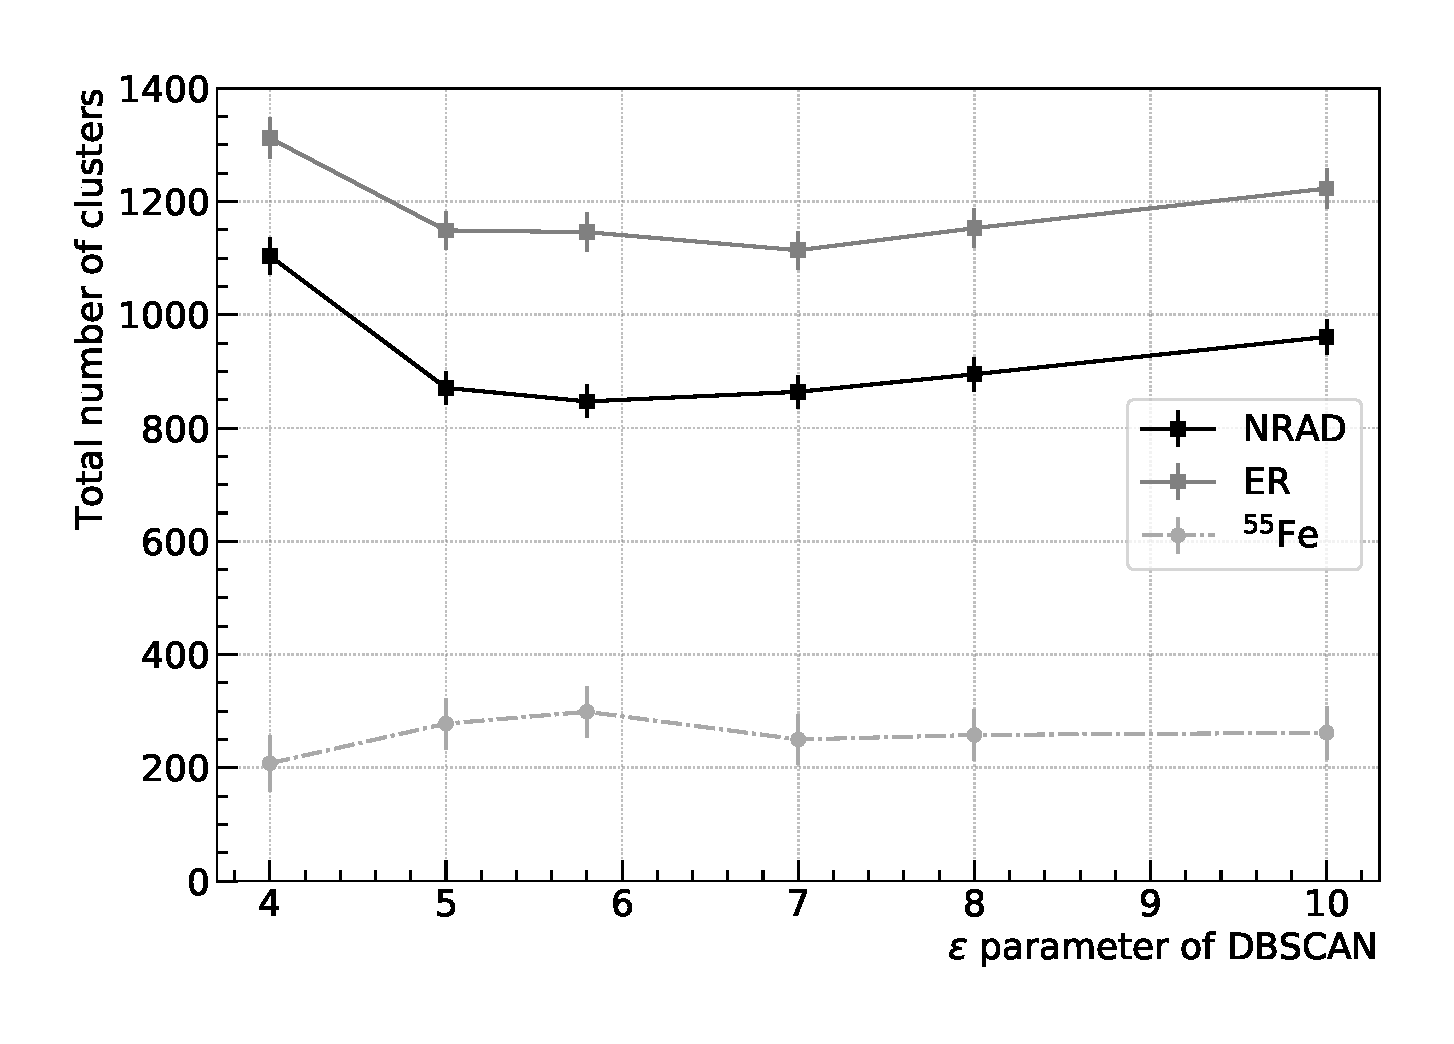
\includegraphics[width=0.45\textwidth]{TotalEpsScan.pdf}
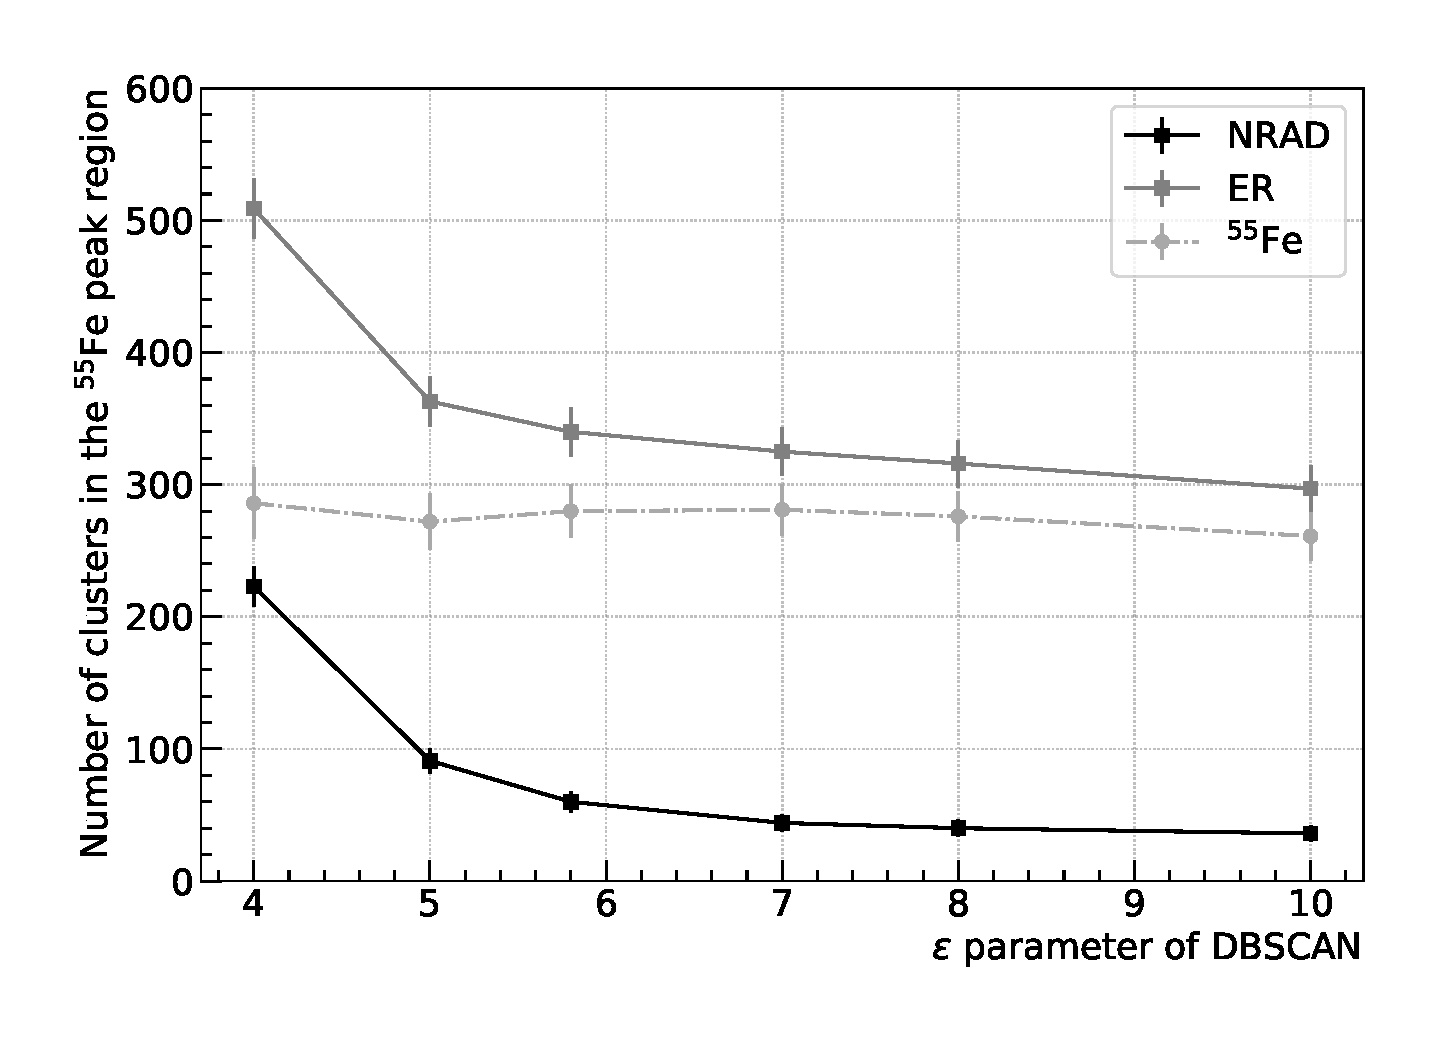
\includegraphics[width=0.45\textwidth]{SpotEpsScan.pdf}
\caption{Total number of reconstructed clusters (left) and Spot number (right) as a function of $\epsilon$ for runs with NRAD events only and with $^{55}$Fe + NRAD events.}
\label{fig:epsscan}
\end{figure}


Similarly, a scan over the $N_{min}$ parameter has been performed as shown in Fig.~\ref{fig:minscan}. Applying the same logic as for the $\epsilon$ parameter, the plot on the left indicates a low contamination region for $N_{min}$ values between 20 and 40, and the right plot to a region for $N_{min}$ $\leq$ 30. In both cases, when stable, the difference between the results indicate a number of $\rm ^{55}Fe$ clusters of about 280. %\textcolor{purple}{add an error}.


\begin{figure}[ht]
\centering
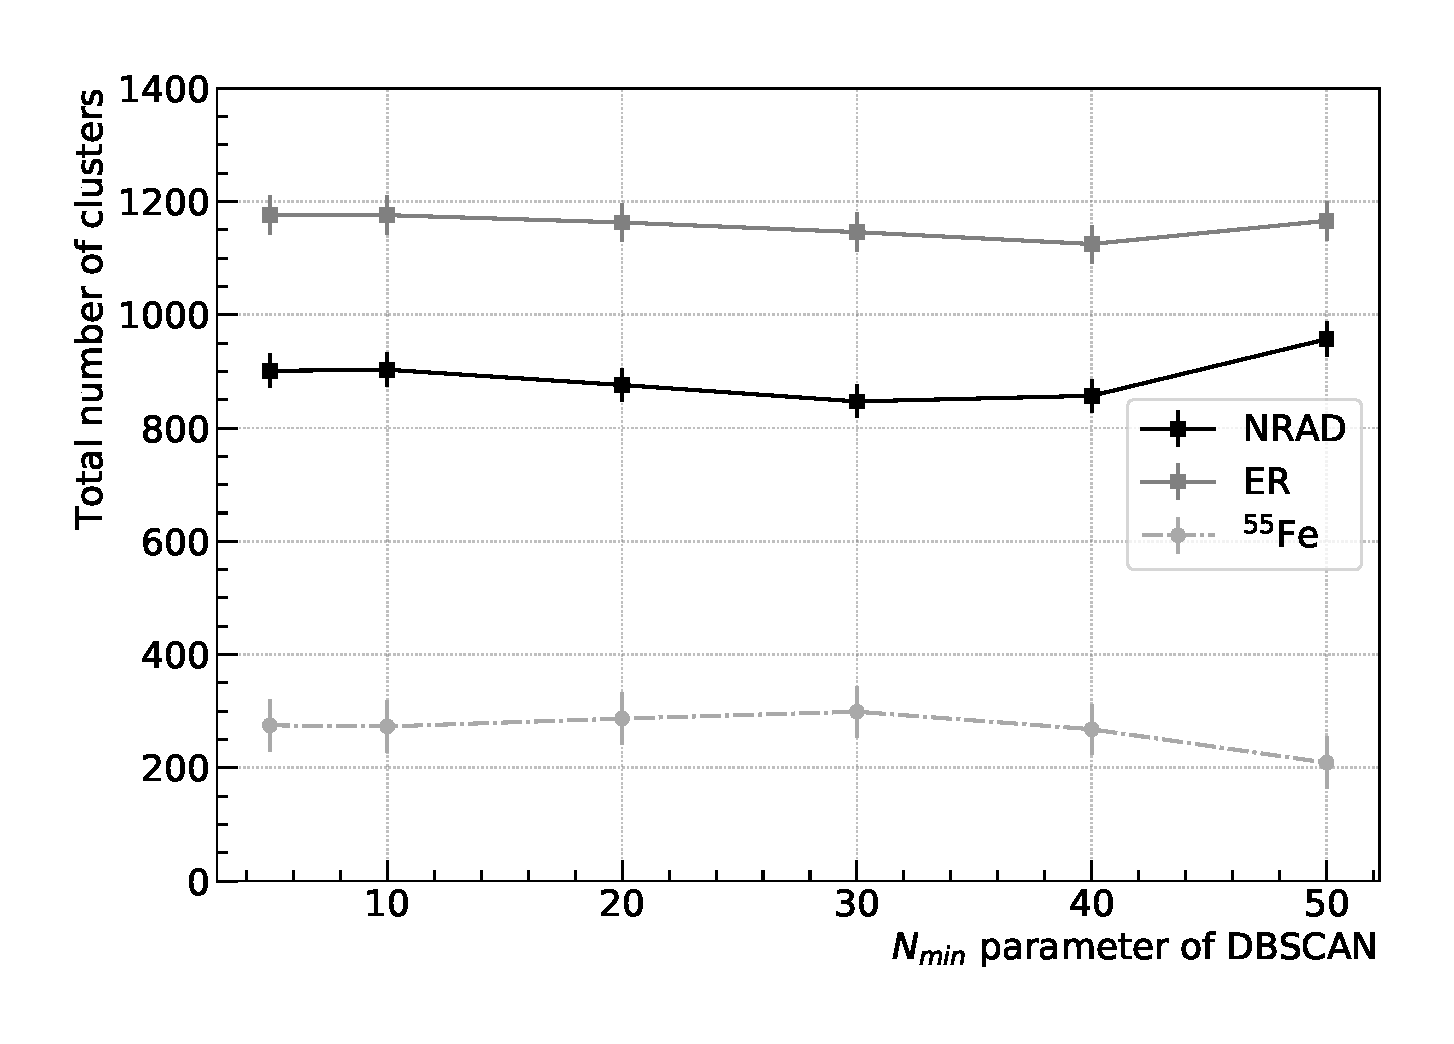
\includegraphics[width=0.45\textwidth]{TotalMinScan.pdf}
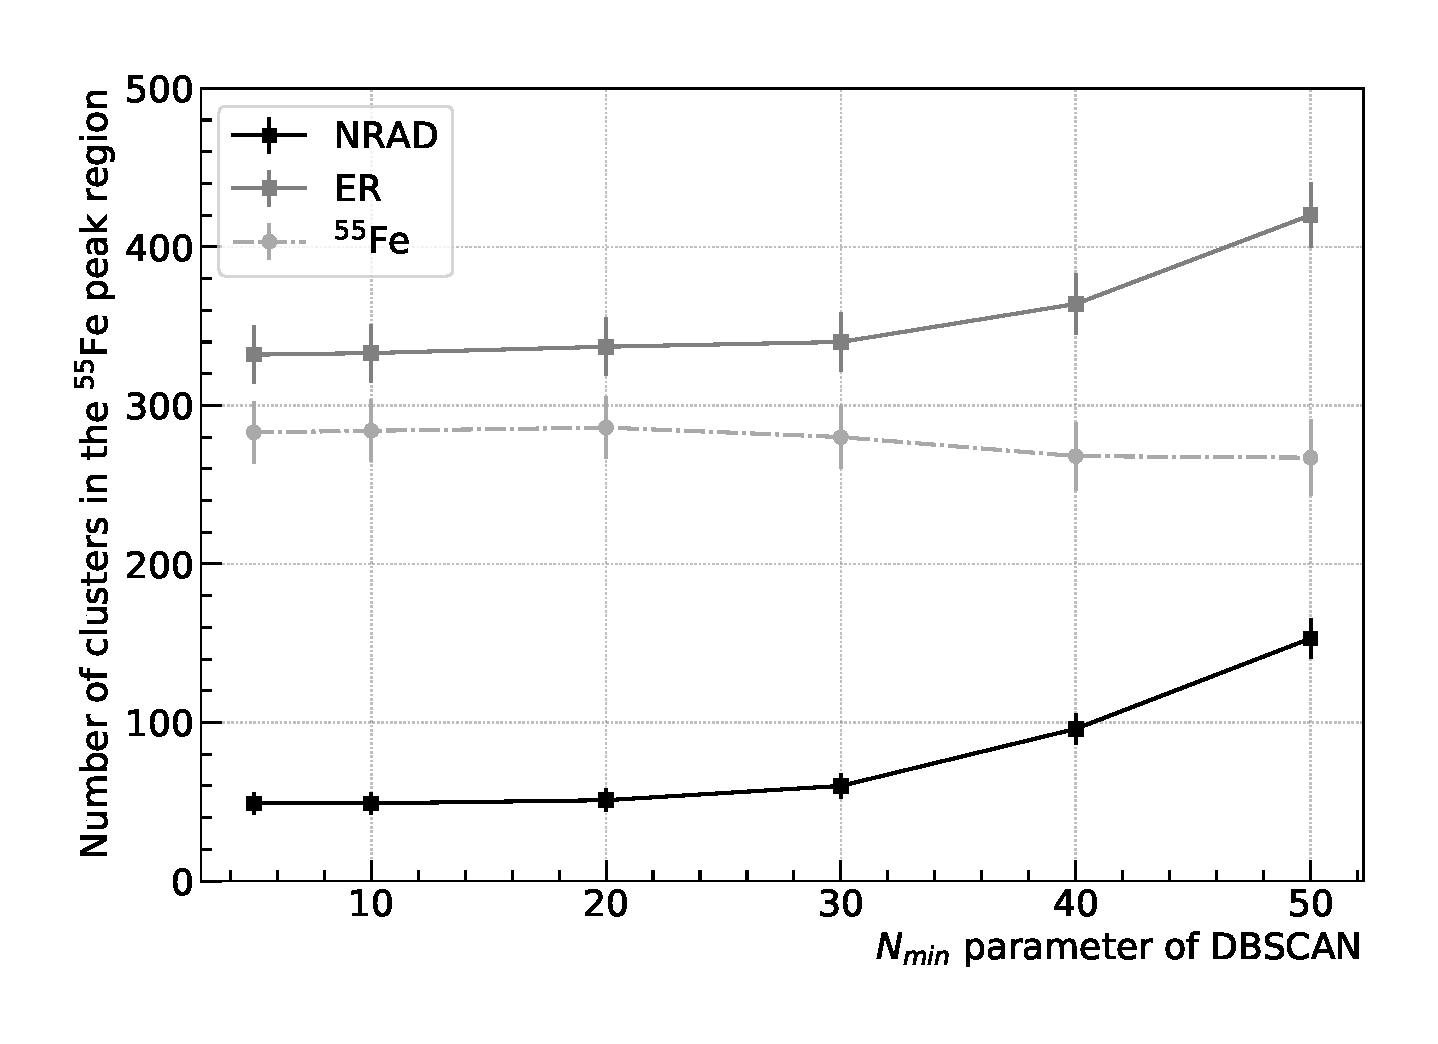
\includegraphics[width=0.45\textwidth]{SpotMinScan.pdf}
\caption{Total number of reconstructed clusters (left) and Spot number (right) as a function of $N_{min}$ for runs with NRAD events only and with $^{55}$Fe + NRAD events.}
\label{fig:minscan}
\end{figure}

Finally, energy resolution has also been measured in function of the iDBSCAN parameters.
Values around 12.2\% have been measured for all the $\epsilon$ and $N_{min}$ considered values, with negligible variation. Section \ref{subsec:detres} provides details about the energy resolution measurement. 

%\section{CYGNO's density-based clustering compared to the previous algorithm}
%\section{CYGNO's DBSCAN compared to the previous algorithm}
\section{iDBSCAN and NNC comparison}
\label{sec:algoComp}


\subsection{Electronic noise, natural radioactivity and $\rm ^{55}Fe$ energy spectra}

%In this section a comparison between NNC and iDBSCAN is carried out. 
The well-known energy deposition signature of 5.9 keV photons coming out from the $\rm ^{55}Fe$ source is exploited in order to evaluate the detection efficiency and background rejection of both methods. While the ER dataset will be used for signal characterization, EN and NRAD datasets will be deployed for background rejection measurements.
%In this section such parameter is used to select clusters with slimness greater than 0.4.
%Therefore, clusters generated by EN, NRAD and $\rm ^{55}Fe$ photons were analyzed.
The EN acquired data produces low energy clusters with a distribution squeezed in the region below 500 photons as shown in Fig. \ref{fig_compnoise}, NRAD produces an energy distribution widely spread by a heavy tail component as shown in Fig.~\ref{fig_compcosmic} while ER forms an additional narrow distribution centered at around 3000 photons as shown in Fig.~\ref{fig_compfe}.
In this last case, the energy spectrum is composed of background and $^{55}$Fe induced deposits and, therefore, to reconstruct the $^{55}$Fe energy distribution, the background distribution should be subtracted. All the distributions were generated with the same amount of images, 864 of them, except for the iDBSCAN distributions of Fig. \ref{fig_compnoise} which used 6478 images, in order to collect enough EN-clusters, which occur at a low rate.  
Additionally, the signal purity is enhanced accounting for the cluster aspect ratio, called slimness, defined as the ratio between the minor axis (width) and major axis (length) of each cluster.

Figure \ref{fig_compnoise} compares the energy spectrum of clusters generated by NNC with those generated by iDBSCAN for EN events without and with a selection based on the slimness parameter, considering only clusters with slimness greater than 0.4 for the later case. The computed numbers of EN-clusters per image for NNC and iDBSCAN were 4.61 $\pm$ 0.07 and $(9 \pm 4)\times 10^{-4}$, respectively.
Regarding NNC, EN-clusters dominate the background rate for energies below 500 photons which can be noticed by comparing the EN energy distribution of Fig. \ref{fig_compnoise} with that of the NRAD shown in Fig. \ref{fig_compcosmic}. Slimness selection decreases the number of clusters per image to 3.80 $\pm$ 0.07 and $(5 \pm 3)\times 10^{-4}$ for NNC and iDBSCAN, respectively. Therefore, when compared to NNC, iDBSCAN is able to reduce the number of EN-clusters per image by a  
%\textcolor{purple}{a factor $(5\div7)\times 10^3$}
factor of $(5\div7)\times 10^3$.
%$(5.1\pm2.3)\times 10^3$ and $(7.6\pm4.6)\times 10^3$ for the cases without and with slimness cut, respectively.

\begin{figure}[ht]
\centering
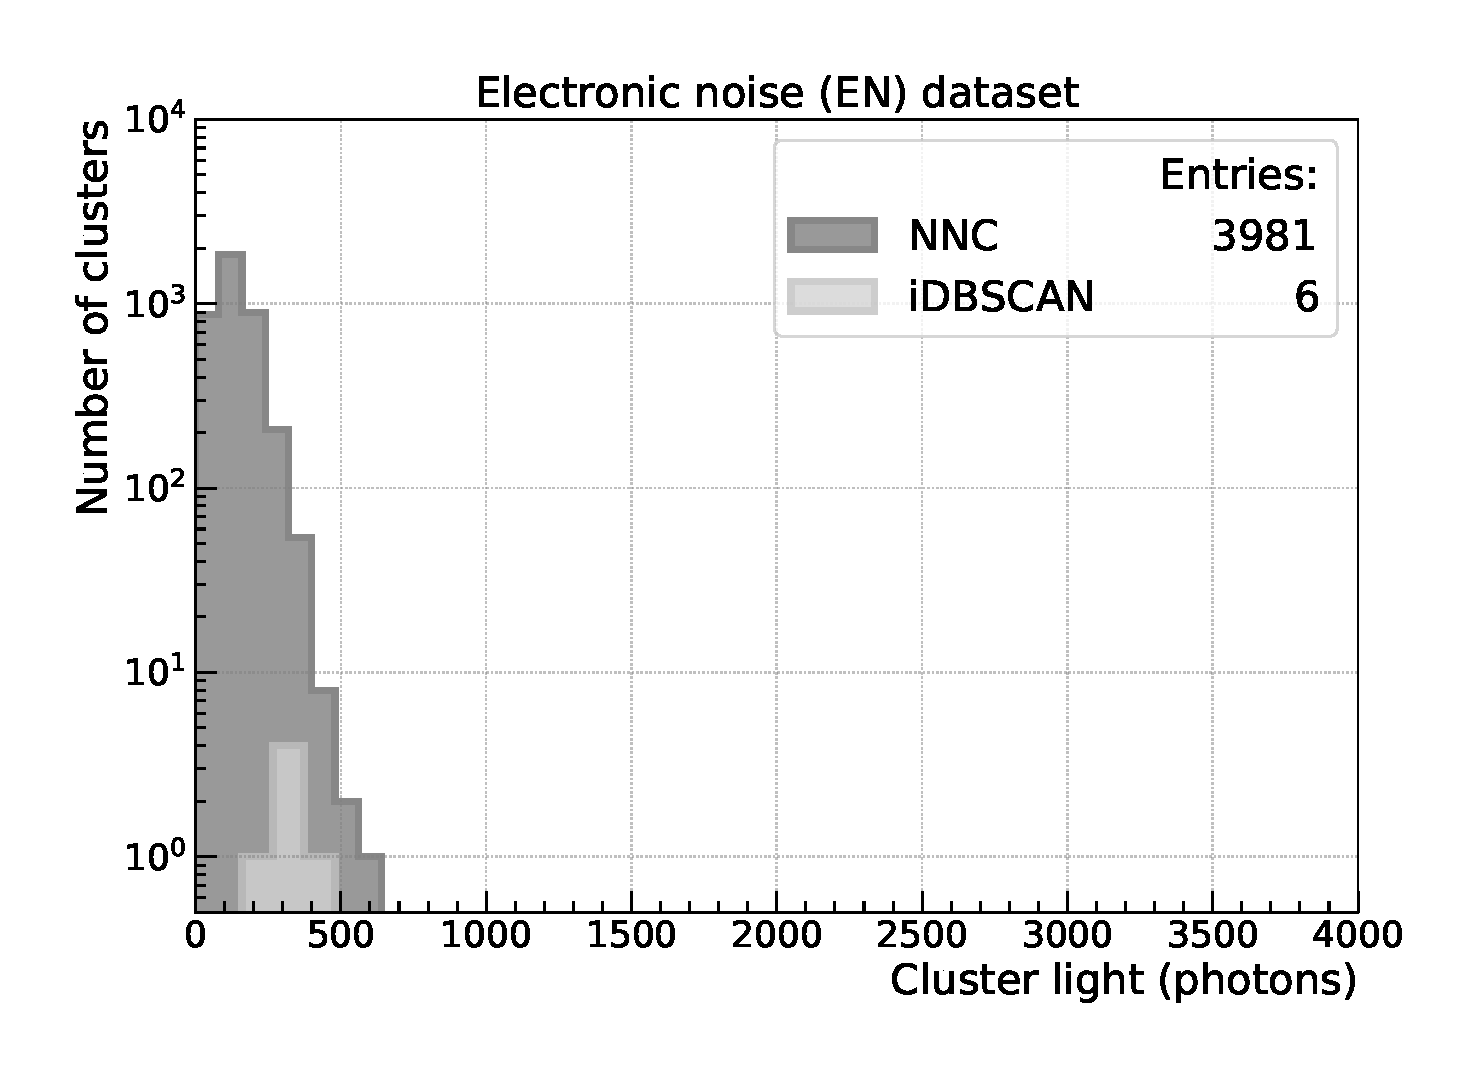
\includegraphics[width=0.45\textwidth]{LigthYield_No_wo.pdf}
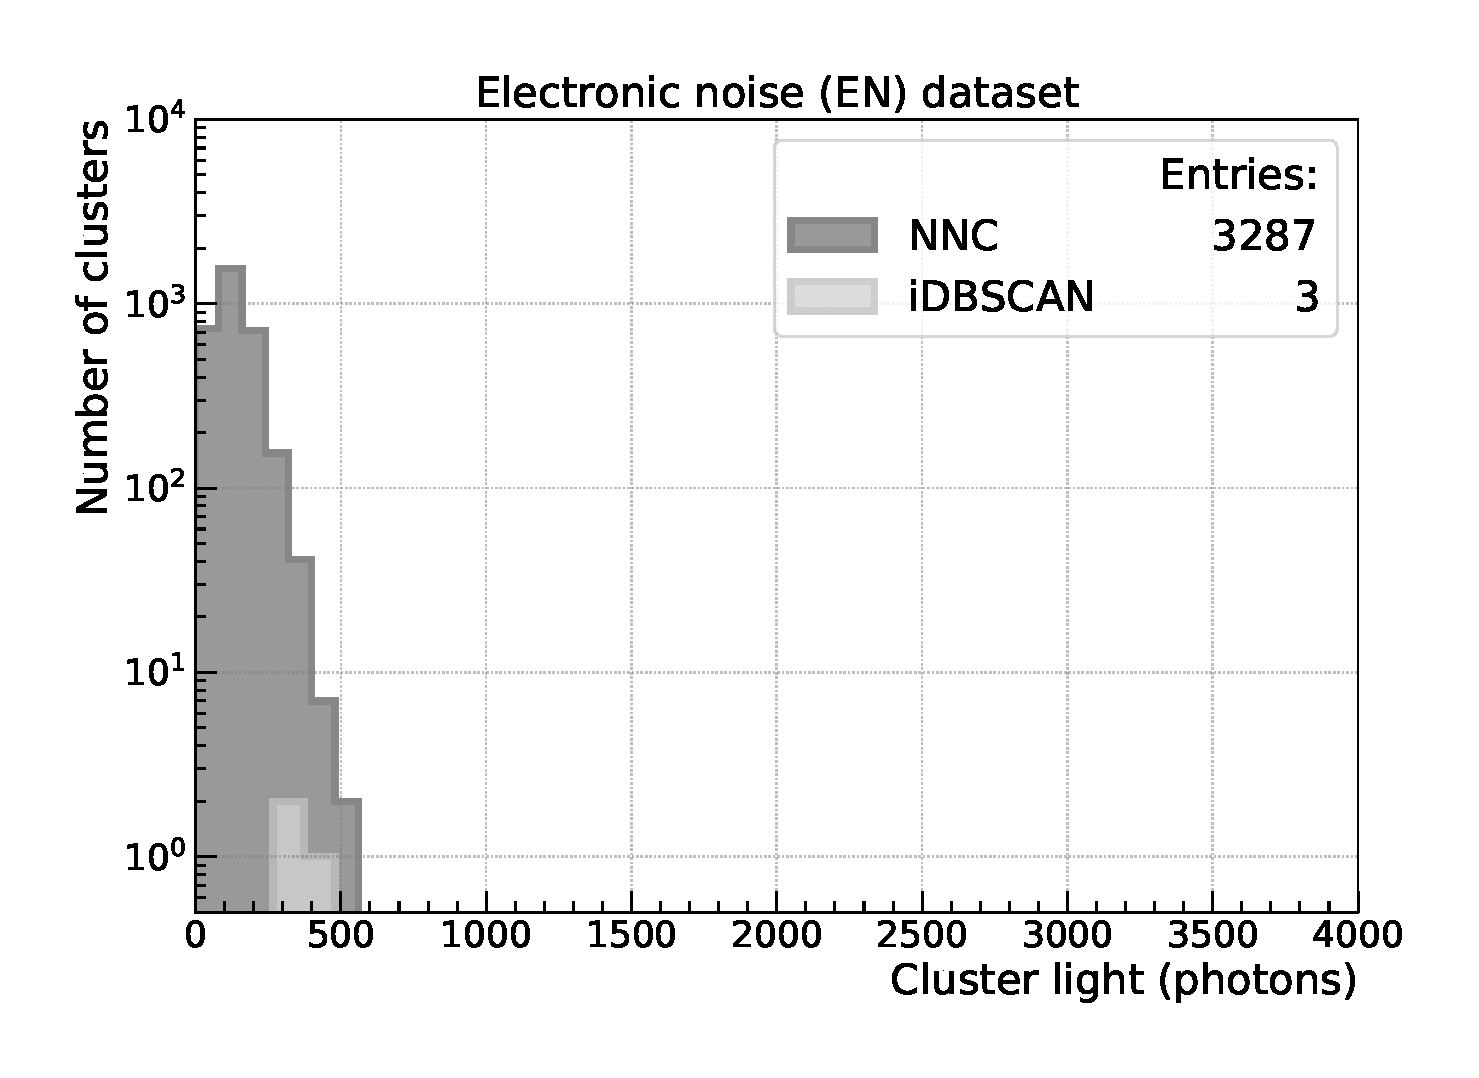
\includegraphics[width=0.45\textwidth]{LigthYield_No_Slim.pdf}
\caption{Clusters energy distribution for NNC and iDSBSCAN applied to the EN dataset, without (left) and with (right) a selection on the slimness.}
\label{fig_compnoise}
\end{figure}


Figure~\ref{fig_compcosmic} presents the energy distributions for the NNC and iDBSCAN clusters using the NRAD dataset without (left) and with (right) a selection on slimness.
iDBSCAN presents a clear peak evolution around 300 photons while NNC accumulates clusters with lower energies. As mentioned before, for NNC this region is highly populated by EN-clusters.
iDBSCAN reduces the number of background events in the region between 2000 and 4000 photons, which is the region where the $\rm ^{55}Fe$ events are expected to be, as mentioned before, providing better background rejection for low energy events as for the 5.9 keV photons.
On the right of Fig.~\ref{fig_compcosmic}, the distribution of light, only considering clusters with slimness greater than 0.4 is shown. As can be observed, this operation has reduced even more the number of background events in the $\rm ^{55}Fe$ region. 
However, for the lower energy region, the number of background clusters has not changed much, causing iDBSCAN to maintain a better background rejection efficiency when compared to NNC.


\begin{figure}[ht]
\centering
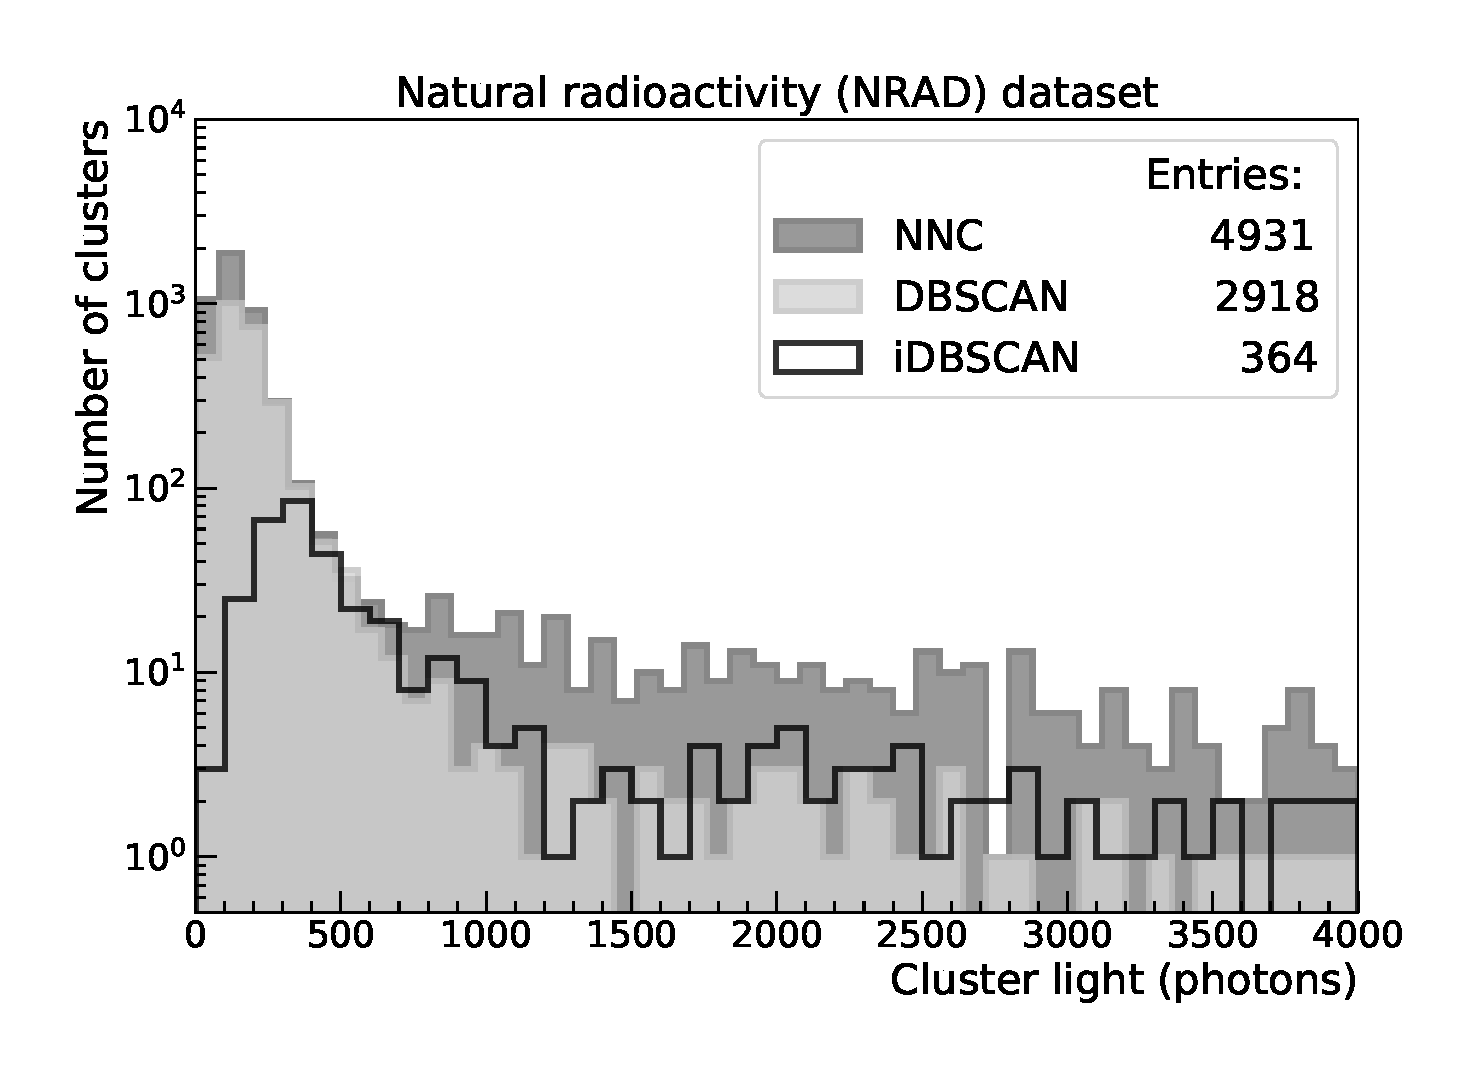
\includegraphics[width=0.45\textwidth]{LigthYield_Cos_wo.pdf}
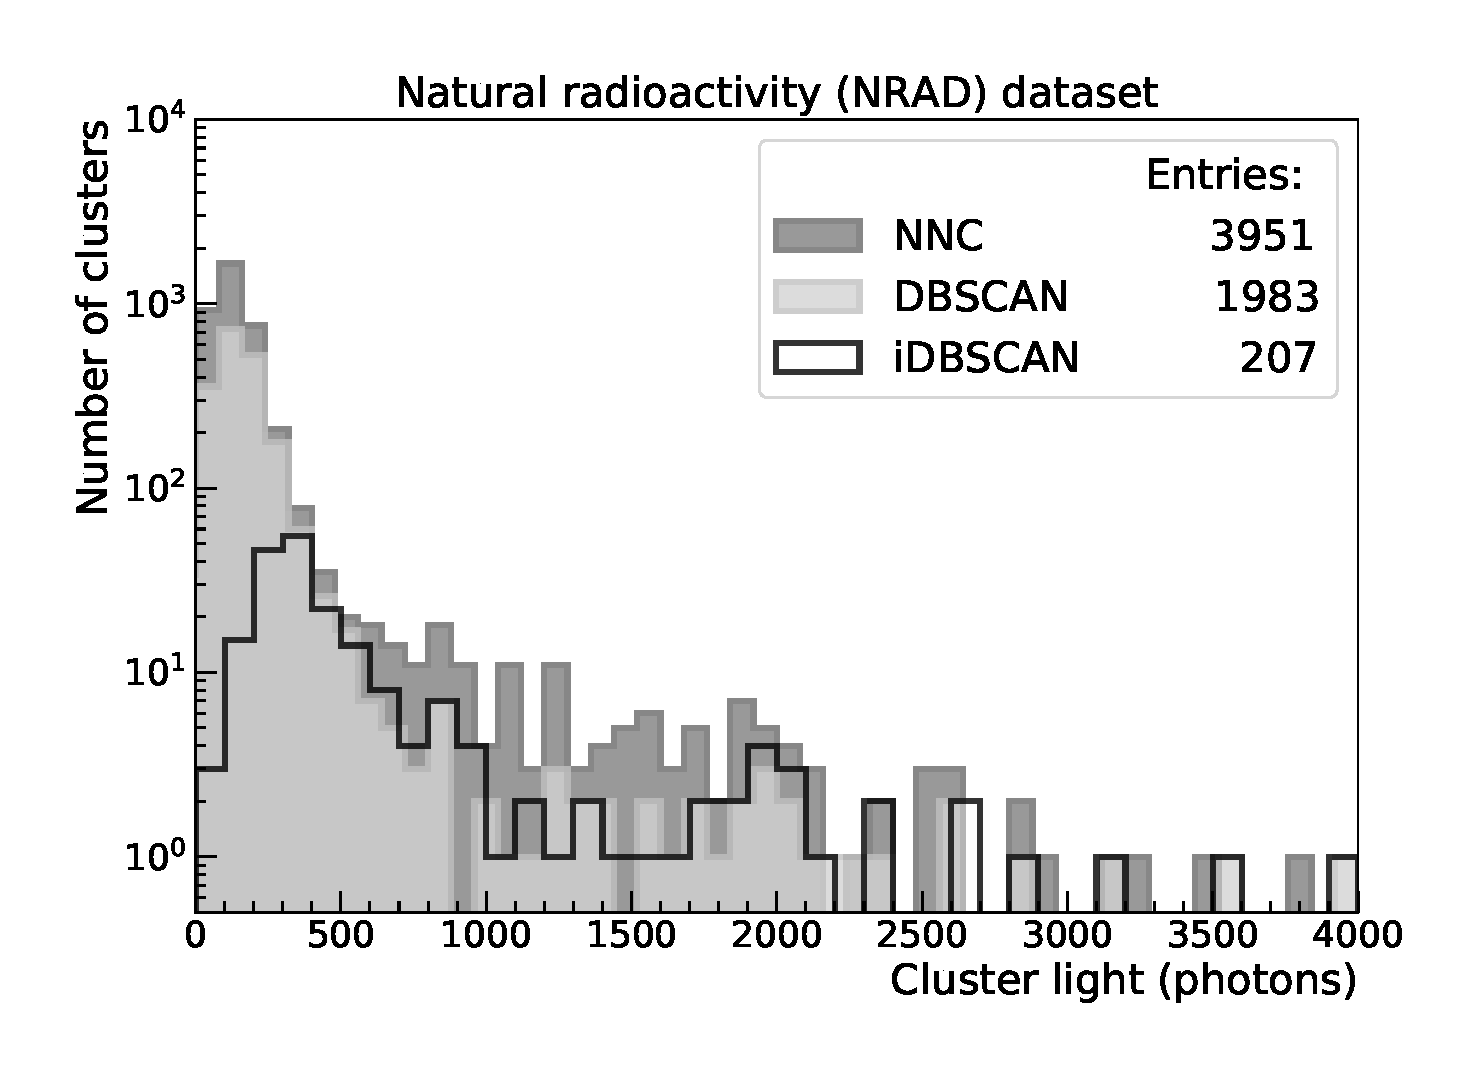
\includegraphics[width=0.45\textwidth]{LigthYield_Cos_Slim.pdf}
\caption{Clusters energy distribution for NNC and iDSBSCAN applied to the NRAD dataset, without (left) and with (right) a selection based on the slimness.}
\label{fig_compcosmic}
\end{figure}

Figure~\ref{fig_compfe} shows the results of the same analysis performed on the ER dataset. In this case, the  sum of the distribution obtained in the NRAD sample and the one from $^{55}$Fe interactions is expected. As shown, both clustering algorithms are sensitive to the 5.9 keV photon events. However, as commented previously, a higher purity level is achieved using iDBSCAN.
After applying the slimness threshold, as shown in the right plot of Fig.~\ref{fig_compfe}, the NNC and iDBSCAN  $^{55}$Fe peaks get closer indicating that both methods have similar detection efficiency considering that the number of $^{55}$Fe spots found by each method is practically the same.  

\begin{figure}[ht]
\centering
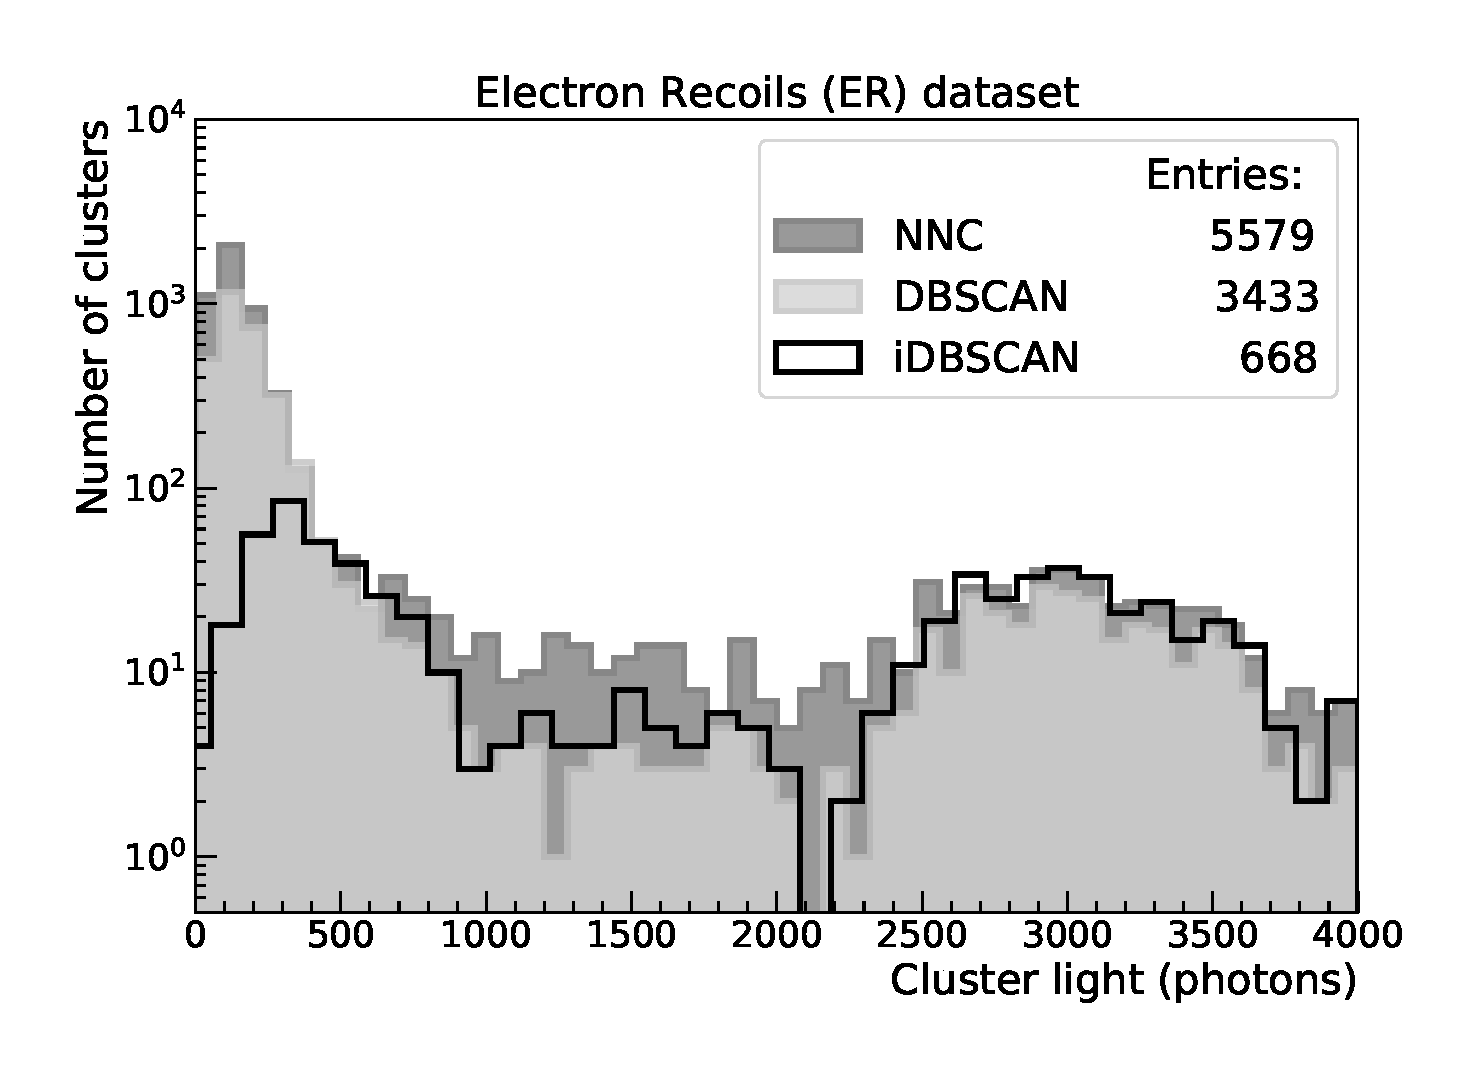
\includegraphics[width=0.45\textwidth]{LigthYield_Fe_wo.pdf}
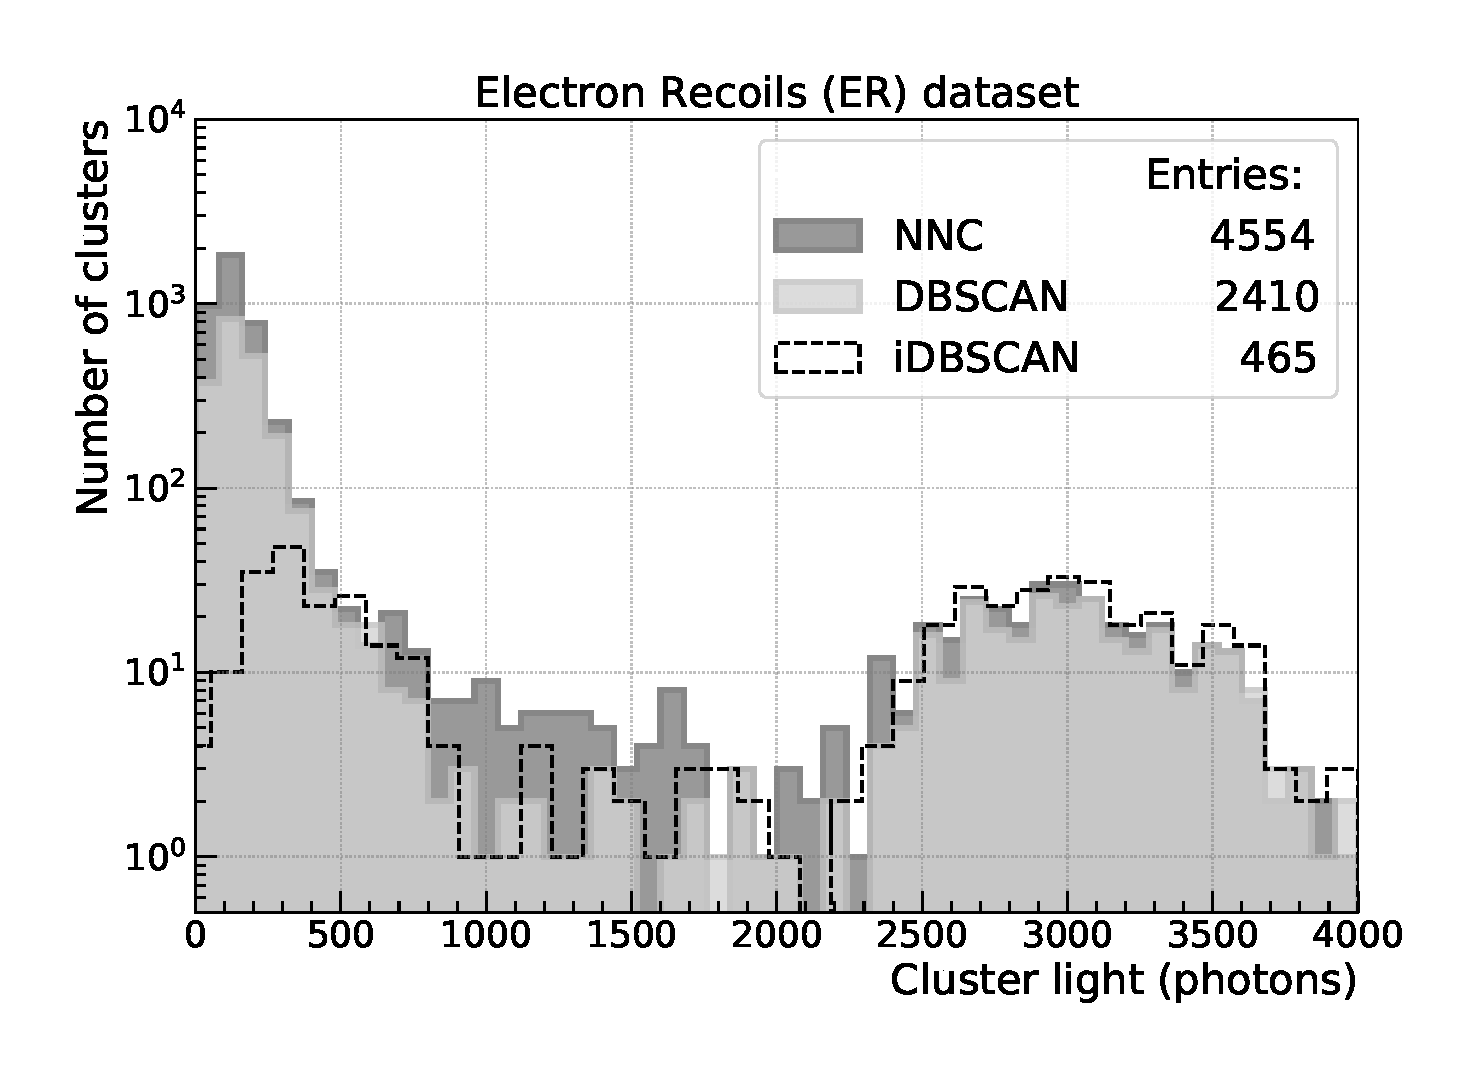
\includegraphics[width=0.45\textwidth]{LigthYield_Fe_Slim.pdf}
\caption{Clusters energy distribution for NNC and iDSBSCAN applied to the ER dataset, without (left) and with (right) a selection based on the slimness.}
\label{fig_compfe}
\end{figure}




\subsection{Slimness selection optimization}
Figure \ref{fig_cdf_slim} shows the slimness cumulative distribution of clusters for an interval between zero and one applied to the NRAD and ER datasets.
NNC and iDBSCAN cases are shown on the left and right plots, respectively.
As it is possible to see, in both cases, $^{55}$Fe spots tend to have slimness higher than about 0.4.
This variable can be used in conjunction with energy measurement to discriminate $^{55}$Fe spots from background clusters.
In this section the value of slimness will be swept so that it is possible to choose the most suitable value for its use as an event selection parameter as well as to evaluate its impact when applied together with the energy measurement.
%In this section, the slimness value will be swept the impact of applying different values of slimness for selecting $^{55}$Fe spots is evaluated. 


\begin{figure}[ht]
\centering
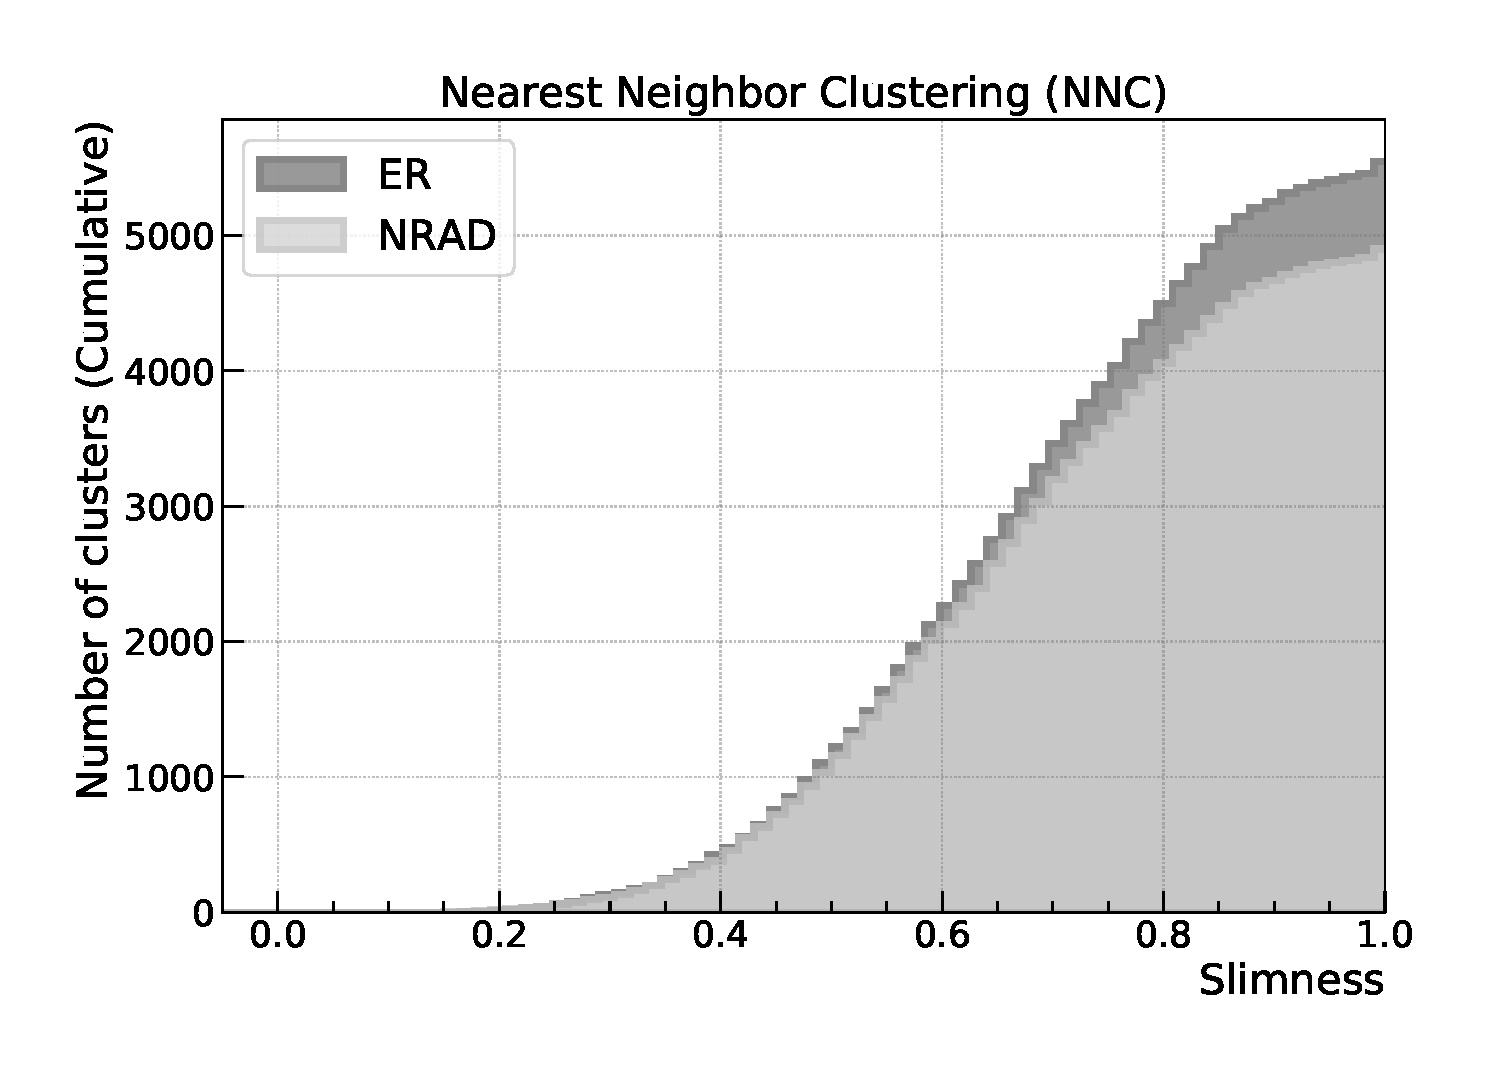
\includegraphics[width=0.45\textwidth]{CDF_Slimness_2D.pdf}
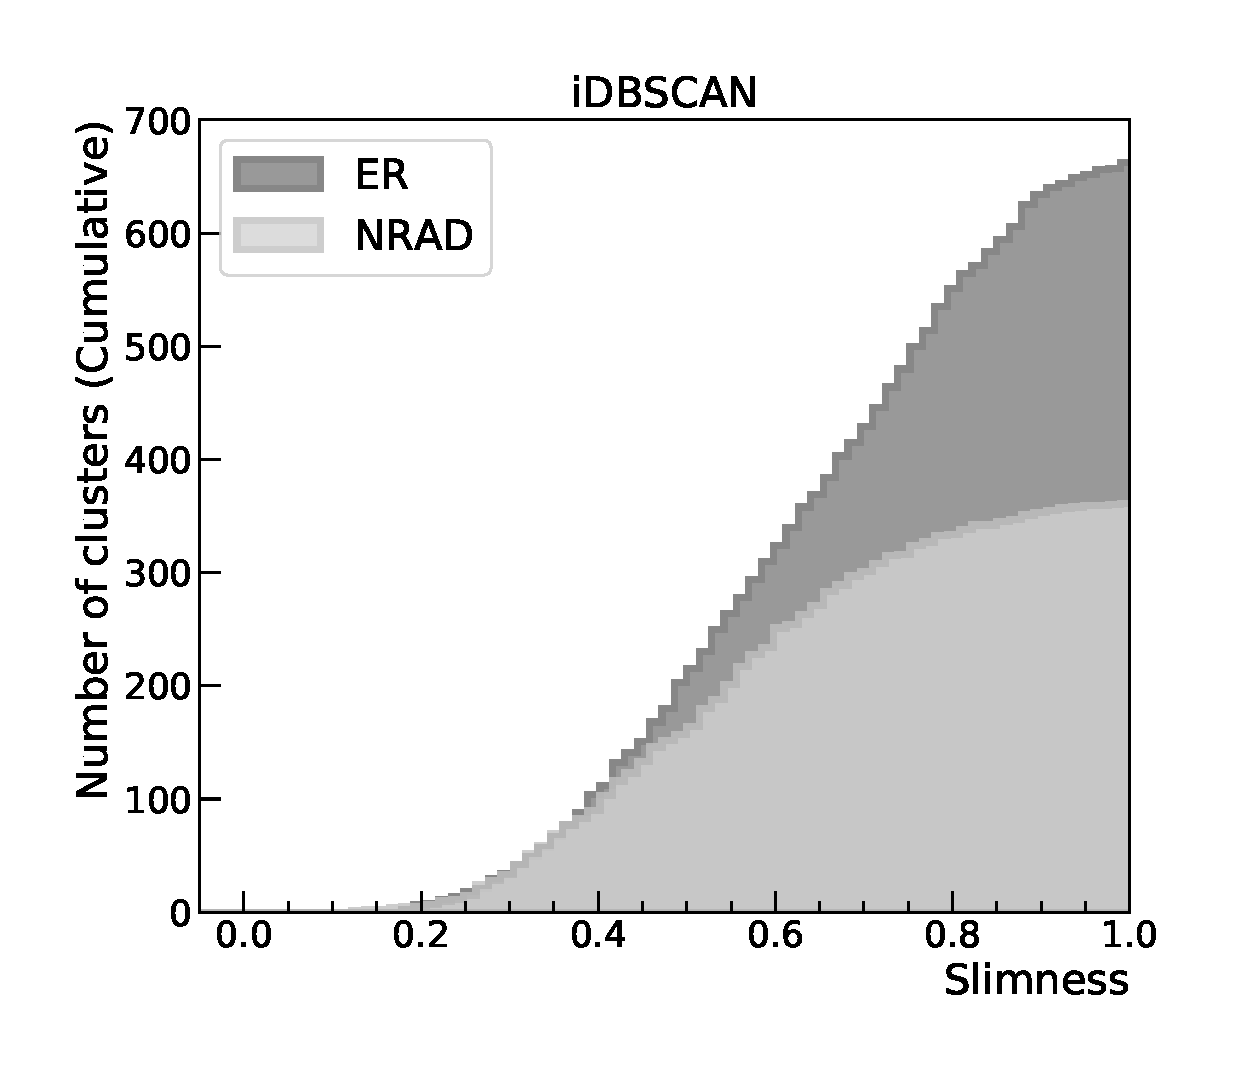
\includegraphics[width=0.45\textwidth]{CDF_Slimness_3D.pdf}
\caption{Cumulative distribution of the slimness for NRAD and $\rm ^{55}Fe$+NRAD data, for NNC (left) and iDSBSCAN (right).} 
\label{fig_cdf_slim}
\end{figure}


In order to evaluate the signal efficiency and purity as a function of the slimness selection for the two algorithms,
%algorithms behavior as a function of slimness,
which should return a purer cluster sample given the differences between the $^{55}$Fe and natural radioactive tracks topologies, the number of clusters within the selected $^{55}$Fe energy region (from 1500 to 4500 photons) was measured for various slimness threshold values (X $\geqslant$ x) as shown in Fig.~\ref{fig_slim_scan} for the NNC (left) and iDBSCAN (right) algorithms.
According to these curves, iDBSCAN finds a similar number of clusters in the $^{55}$Fe region when compared to NNC for slimness below 0.4, given by the difference between the black and gray curves, but with lesser contamination (gray curve).

Considering that the $^{55}$Fe clusters produce an intensity that follows a Gaussian distribution with an average value of about 3000 photons and standard deviations of 550 and 371, for NNC and iDBSCAN respectively (see Fig. \ref{fig_CosFe}), then more than 99\% of the $^{55}$Fe clusters are selected between 1500 and 4500 photons.
%, which are equivalent to about 2.7 standard deviations for NNC and 4.0 for iDBSCAN.
On the other hand, for the same region, the subtraction of the natural radioactivity events between the $^{55}$Fe and NRAD acquisition runs has a mean value equal to zero but a fluctuation of about 23 (14) and 11 (7) clusters for slimness equal to 0.0 (0.4), for NNC and iDBSCAN respectively. Therefore, the dashed line of Fig. \ref{fig_slim_scan} is composed mainly of $^{55}$Fe events plus few background events produced by the statistical fluctuation that occurs in the process of subtracting natural radioactivity.
As can be noticed by observing Fig. \ref{fig_compcosmic}, iDBSCAN tends to have less background contamination than NNC, reducing the statistical uncertainty related to the background subtraction. This effect is also shown by the shaded band drawn around the dashed lines of Fig. \ref{fig_slim_scan}.

\begin{figure}[ht]
\centering
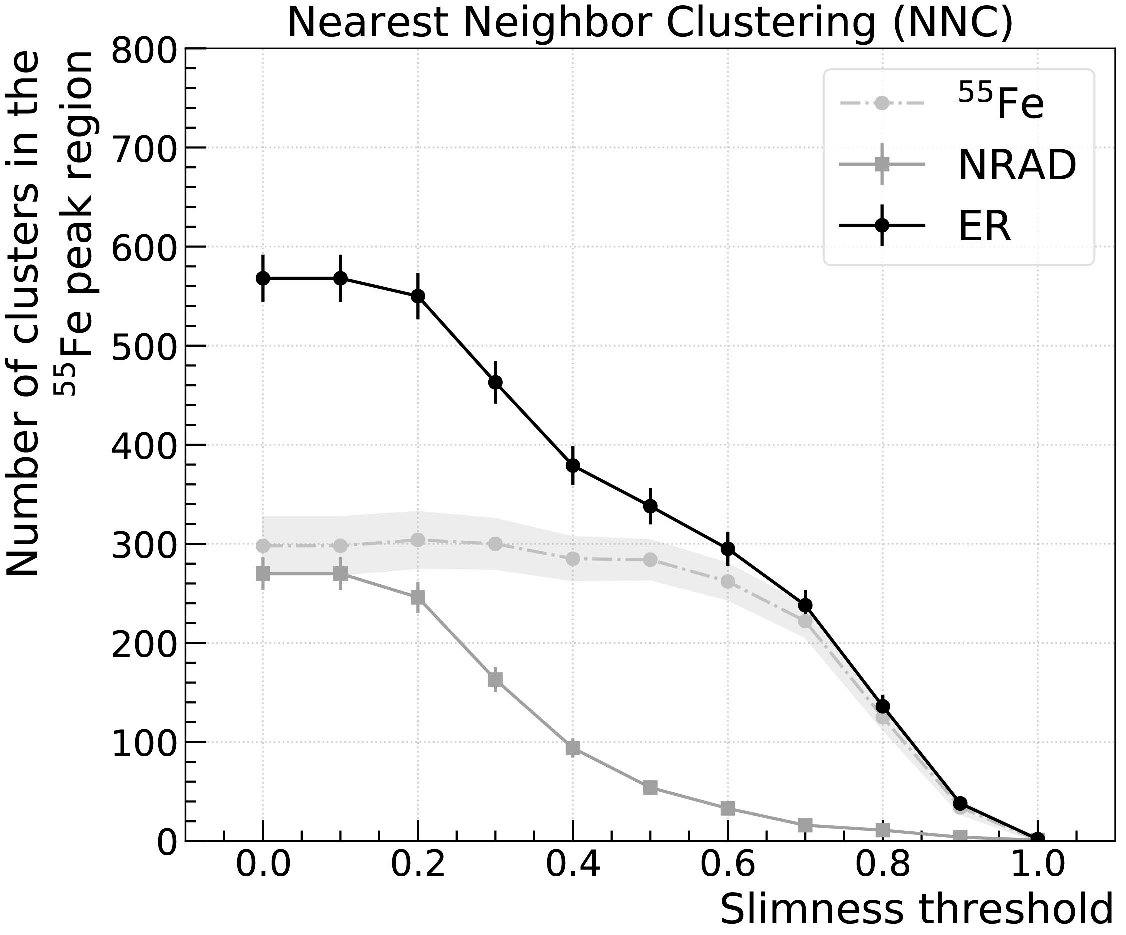
\includegraphics[width=0.45\textwidth]{NNC_ScanSlim.pdf}
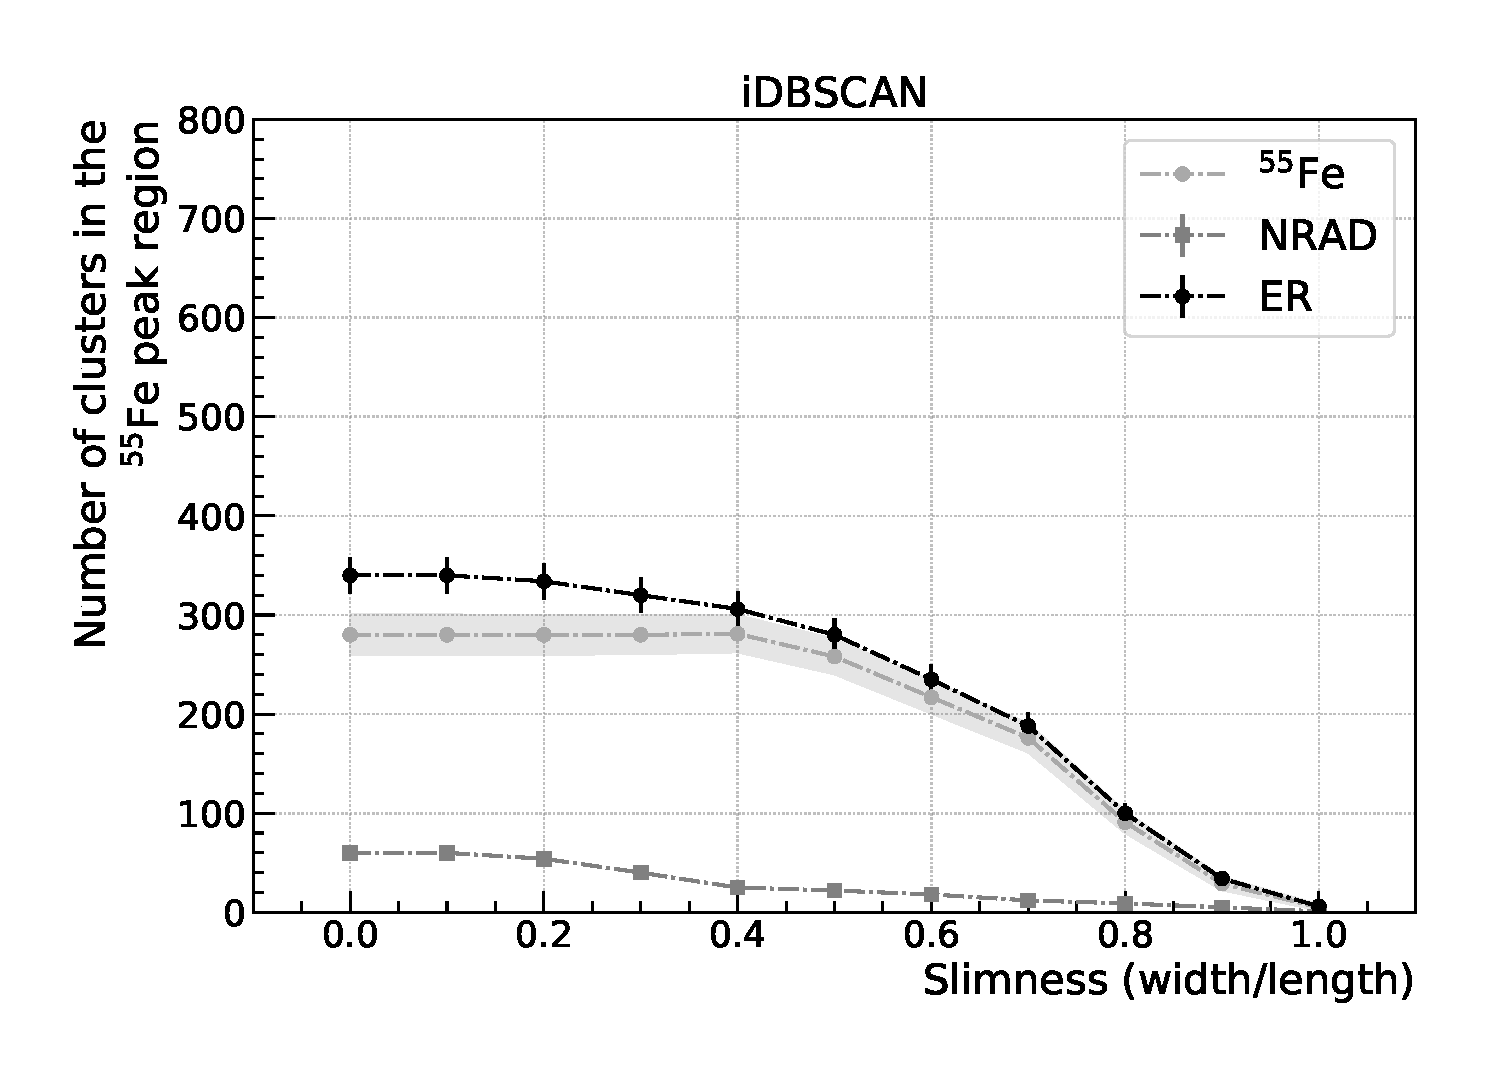
\includegraphics[width=0.45\textwidth]{I2DBSCAN_Scanslim.pdf}
\caption{Scan in the number of clusters on the $\rm ^{55}Fe$ peak region (between 1500 and 4500 photons) when changing the threshold on the slimness for NRAD and $\rm ^{55}Fe$+NRAD data, for NNC (left) and iDSBSCAN (right).} 
\label{fig_slim_scan}
\end{figure}

%\newpage

Based on the measurements of Fig.~\ref{fig_slim_scan}, the impact of the slimness parameter can be assessed by measuring selection efficiency ($\rm \varepsilon_{sel}$) and fake events ($\rm F_{evts}$), as defined below:
\begin{itemize}
    \item $\rm \varepsilon_{sel}$: number of clusters found in the ER dataset ($\rm nFe$) subtracted by the number of clusters found in the NRAD dataset ($\rm nRd$) divided by the maximum value of the $\rm nFe-nRd$ subtraction among all slimness values (see Equation~\ref{eq:01});
    
    \begin{equation}
       {\rm \varepsilon_{sel} = \left( {\frac{{nFe - nRd}}{{\max \left( {nFe - nRd} \right)}}} \right)}
       \label{eq:01}
    \end{equation}

    
    \item $\rm F_{evts}$: ratio between the number of clusters found in the NRAD dataset ($\rm nRd$) and the number of clusters found in the ER dataset ($\rm  nFe$) (see Equation~\ref{eq:02}a). This measure can also be understood in terms of background rejection ($\rm B_{rj}$) as shown by Equation~\ref{eq:02}b;
    
    %\begin{equation*}
    %    {Fa = \left( {\frac{{nCo}}{{nFe}}} \right)
    %    \times 100}
    %    \label{eq:02}
    %\end{equation*}
    
\end{itemize}
\begin{equation}
    \begin{array}{*{20}{c}}
   \begin{array}{*{20}{c}}
   {\rm F_{evts} = \left( {\frac{{nRd}}{{nFe}}} \right)}  \\
\end{array} ~~(a) & {, ~~~} & {\rm B_{rj} = 1 - F_{evts} }  \\
\end{array} ~~(b)
\label{eq:02}
\end{equation}

Figure~\ref{fig_cdf_slim} shows that for slimness below 0.4
the efficiency for background events is very small, while most of the $^{55}$Fe events are retained.
%Above this value the number of $^{55}$Fe clusters will also tend to decrease, indicating a loss of efficiency.
Table~\ref{tab:dvNccComp} shows the computed $\rm \varepsilon_{sel}$ and $\rm F_{evts}$ for both clustering methods and different thresholds on the slimness variable ranging from 0.0 to 0.8.  For the high efficiency region ($\geq 0.94$), occurring for slimness values from 0.0 to 0.4, iDBSCAN achieved a lower fake event probability, always about 3 times less than NNC. For slimness greater than or equal to 0.6 both methods begin to lose efficiency.
%showed an improvement in false alarm of approximately 65\% in relation to NNC.
%The best results were achieved for slimness of about 0.4: statistically with the same efficiency as for lower values of slimness, but with a better background rejection performance. 
For slimness greater than 0.4, the signal is still almost 100$\%$ efficient, while the background is reduced by a factor 1/4.



% Please add the following required packages to your document preamble:
% \usepackage{multirow}
%\begin{table}[ht]
%\small
%\centering
%\caption{Detection Efficiency and Fake Events comparison between NNC and iDBSCAN.}
%\label{tab:dvNccComp}
%\begin{tabular}{c|cc|cc|cc|cc|cc}
%\multirow{2}{*}{\begin{tabular}[c]{@{}c@{}}Slimness\\ (width/length)\end{tabular}} & \multicolumn{4}{c|}{Efficiency (\%)}                     & \multicolumn{4}{c|}{Fake Events (\%)}  & \multicolumn{2}{c}{\begin{tabular}[c]{@{}c@{}}Background\\ rejection\end{tabular}}                  \\
 %                                                                                      & \multicolumn{2}{c|}{iDBSCAN} & \multicolumn{2}{c|}{NNC}   & \multicolumn{2}{c|}{iDBSCAN} & \multicolumn{2}{c|}{NNC} & \multicolumn{2}{c}{improvement (\%)}   \\ \hline \hline
%0.0                                                                                    & ~~97.8  & $^{+1.2}_{-2.5}$ & ~~96.6 & $^{+1.6}_{-2.8}$ & 13.6  & $^{+4.3}_{-3.4}$ & 38.5 & $^{+4.5}_{-4.4}$ & 40.5 & $^{+10.6}_{-~9.6}$\\
%0.2                                                                                    & ~~98.5  & $^{+1.0}_{-2.3}$ & ~~99.3 & $^{+0.6}_{-1.8}$ & 11.8  & $^{+4.2}_{-3.3}$ & 35.5 & $^{+4.6}_{-4.3}$ & 36.8 & $^{+10.0}_{-~8.8}$\\
%0.4                                                                                    & 100.0    & $^{+0.0}_{-1.4}$ & 100.0   & $^{+0.0}_{-1.3}$ & ~~5.5   & $^{+3.2}_{-2.2}$ & 14.5 & $^{+4.2}_{-3.4}$ & 10.4 & $^{+~6.2}_{-~4.7}$ \\
%0.6                                                                                    & ~~79.5  & $^{+4.4}_{-5.3}$  & ~~88.5 & $^{+3.3}_{-4.2}$ & ~~3.6   & $^{+3.3}_{-1.9}$ & ~~6.4  & $^{+3.5}_{-2.4}$ & ~~3.1 & $^{+~5.1}_{-~3.2}$\\
%0.8                                                                                    & ~~33.7   & $^{+5.9}_{-5.5}$ & ~~42.2 & $^{+5.7}_{-5.6}$ & ~~4.2   & $^{+6.1}_{-2.7}$ & ~~3.1   & $^{+4.5}_{-2.0}$ & ~-1.1 & $^{+~3.5}_{-~7.9}$
%\end{tabular}
%\end{table}


\begin{table}[ht]
\small
\centering
\caption{$\rm \varepsilon_{sel}$ and $\rm F_{evts}$ comparison between NNC and iDBSCAN.}
\label{tab:dvNccComp}
\begin{tabular}{c|cc|cc|cc|cc|c}
\multirow{2}{*}{\begin{tabular}[c]{@{}c@{}}\textbf{Slimness}\\ (width/length)\end{tabular}} & \multicolumn{4}{c|}{$\mathbf{\rm \varepsilon_{sel}}$}                     & \multicolumn{4}{c|}{$F_{evts}$}  & \multicolumn{1}{c}{\begin{tabular}[c]{@{}c@{}}$B_{rj} (\%)$\end{tabular}}                  \\
                                                                                       & \multicolumn{2}{c|}{iDBSCAN} & \multicolumn{2}{c|}{NNC}   & \multicolumn{2}{c|}{iDBSCAN} & \multicolumn{2}{c|}{NNC} & \multicolumn{1}{c}{\scriptsize iDBSCAN improvement }   \\ \hline \hline
0.0                                                                                    & 1.00  & $^{+0.00}_{-0.02}$ & 0.98 & $^{+0.01}_{-0.02}$ & 0.18  & $^{+0.04}_{-0.04}$ & 0.48 & $^{+0.04}_{-0.04}$ & ~56.98 $^{+5.15}_{-5.41}$\\
0.2                                                                                    & 1.00  & $^{+0.00}_{-0.02}$ & 1.00 & $^{+0.00}_{-0.01}$ & 0.16  & $^{+0.04}_{-0.04}$ & 0.45 & $^{+0.04}_{-0.04}$ & ~51.67 $^{+4.50}_{-4.73}$\\
0.4                                                                                    & 1.00  & $^{+0.00}_{-0.01}$ & 0.94 & $^{+0.02}_{-0.03}$ & 0.08  & $^{+0.04}_{-0.03}$ & 0.25 & $^{+0.05}_{-0.04}$ & ~22.60 $^{+1.37}_{-1.62}$ \\
0.6                                                                                    & 0.77  & $^{+0.05}_{-0.05}$ & 0.86 & $^{+0.03}_{-0.04}$ & 0.08  & $^{+0.04}_{-0.03}$ & 0.11 & $^{+0.04}_{-0.03}$ & ~03.96 $^{+0.19}_{-0.26}$\\
0.8                                                                                    & 0.32  & $^{+0.06}_{-0.05}$ & 0.41 & $^{+0.05}_{-0.06}$ & 0.09  & $^{+0.07}_{-0.04}$ & 0.08 & $^{+0.06}_{-0.04}$ & -01.00 $^{+0.10}_{-0.06}$
\end{tabular}
\end{table}

The last column of Table \ref{tab:dvNccComp} shows the iDBSCAN background-rejection improvement compared to NNC. 
For slimness equal to 0.4, for example, iDBSCAN has 92\% of background rejection efficiency while NNC has 75\%, leading to a relative improvement of (92-75)/75 $\approx$ 23\%.
%As shown, when slimness is not applied, iDBSCAN might have an improvement over NNC of about 57\% in background rejection efficiency.
%For the first line for example, iDBSCAN has 86\% of background rejection while NNC has 61\% achieving an improvement of (86-61)/61 $\approx$ 41\% in relation to NNC for slimness equal to zero.
%\textcolor{purple}{We should underline that for high detection efficiencies (larger than 95~\%) false alarms of iDBSCAN is always 3 times less than NNC. No cut on slimness can help NCC}

%\subsection{Detector performance using the density-based clustering algorithm}
%\label{sec:detPerf}

%This section presents the measurements of two crucial parameters regarding the detection of low energy and rare particle events: energy resolution and noise background rejection. Results will be given for both  NNC and i2DBSCAN algorithms.

\subsection{Light Yield Resolution}\label{subsec:detres}

%For each algorithm, the energy spectrum  of the total light for the clusters reconstructed within the detector sensitive area were studied. Figure \ref{fig_CosFe} shows the resulting distributions using the NNC algorithm at left and DBSCAN at right.


The detector energy resolution was estimated by a fit to the clusters energy distributions accounting for natural radioactivity and the $^{55}$Fe events. The former was modeled by an exponential function and the latter by a Polya function \cite{bib:rolandiblum}:

\begin{equation}
   P(n)=\frac{1}{b\overline{n}}\frac{1}{k!}\left(\frac{n}{b\overline{n}}\right)^k \cdot e^{-n/b\overline{n}}
   %A\frac{\Gamma(r+k)}{k!\Gamma(r)} p^k (1-p)^r e^{(-x/\lambda)} 
\label{fun:polya}
\end{equation}
where $b$ is a free parameter and $k=1/b-1$. The distribution has $\overline{n}$ as expected value, while the variance is governed by $\overline{n}$ and the $b$ parameter, as follows: $\sigma^2=\overline{n}(1+b\overline{n})$. The total likelihood is given by the sum of the two functions.



Figure~\ref{fig_CosFe} shows the fit results for NCC (left) and iDBSCAN (right) clusters without applying any selection on the slimness parameter.
Based on the computed values, energy resolution were measured to be (18.1 $\pm$ 3.9)\% and (12.2 $\pm$ 1.8)\% for NNC and iDBSCAN respectively, and the energy conversion factor approximately 515 ADC units per keV for both.
Conversion factor and Energy resolution are computed using the \textit{mean} and \textit{sigma} parameters shown in Fig.~\ref{fig_CosFe}. 
The former is given by dividing the \textit{sigma} by the \textit{mean}, while for the latter the \textit{mean} is divided by 5.9 keV (ER energy).
%The former is given by dividing sigma by mean while the later divides mean by 5.9 keV (ER energy).
%

\begin{figure}[ht]
\centering
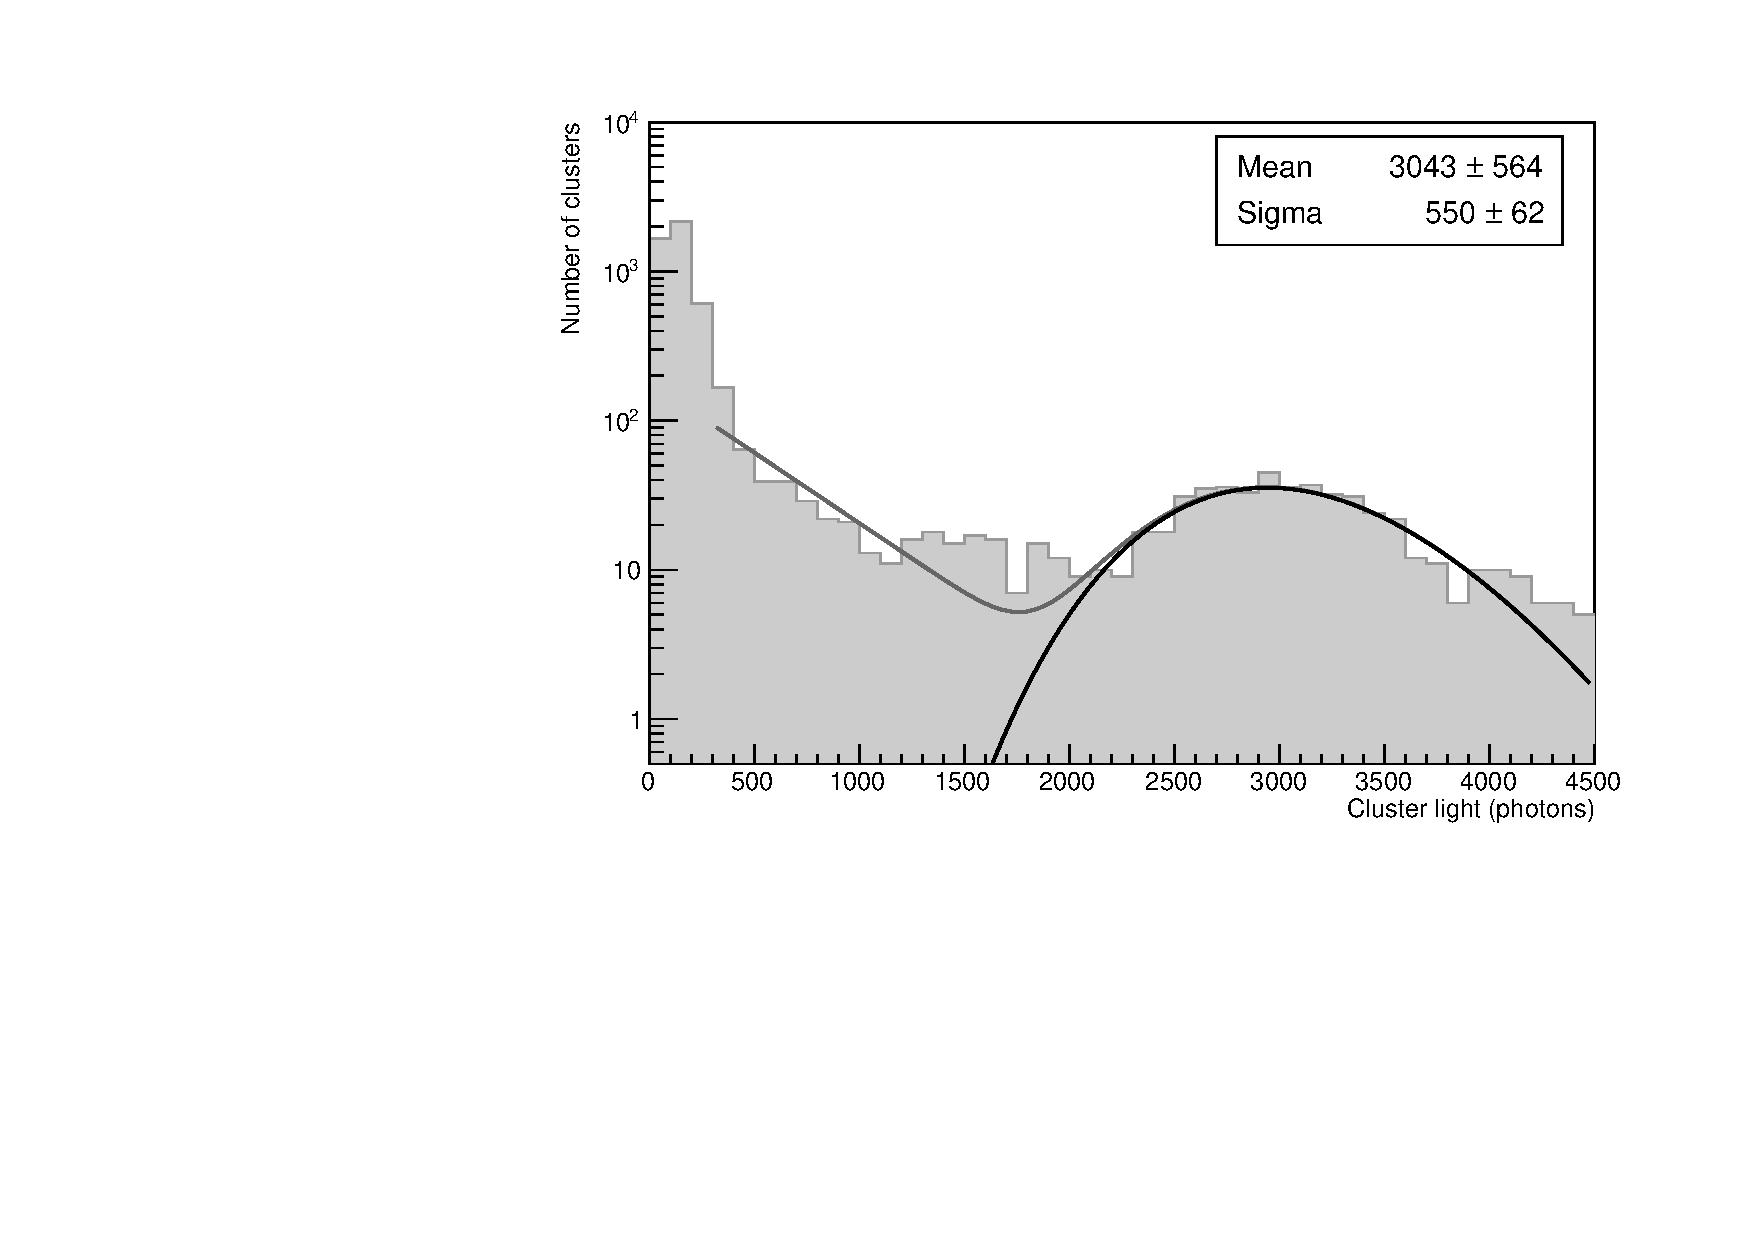
\includegraphics[width=0.44\textwidth]{log_Resolution_NNC_0.pdf}
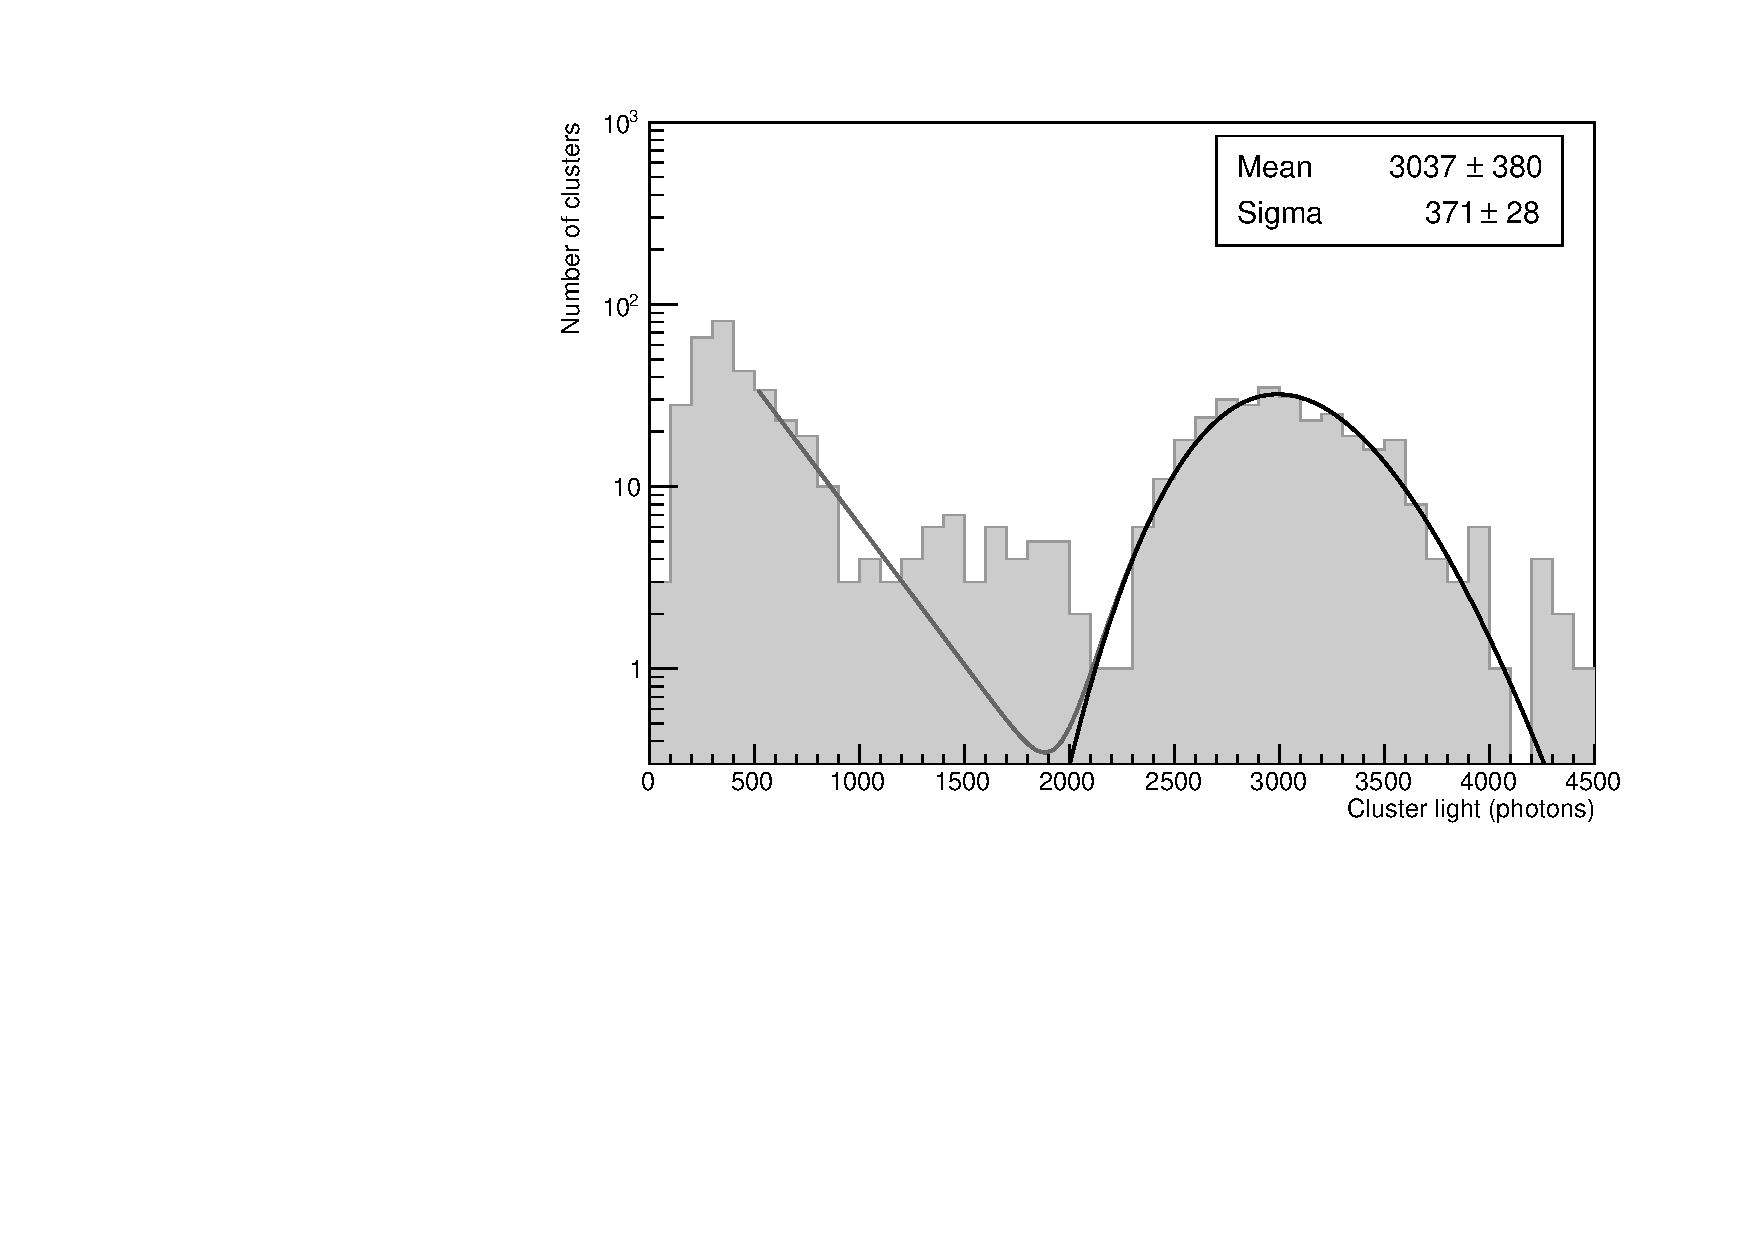
\includegraphics[width=0.44\textwidth]{log_Resolution_DB_0.pdf}
\caption{Results of the fit applied to the NNC (left) and iDBSCAN (right) energy distributions.}
\label{fig_CosFe}
\end{figure}


%
%where n represents the number of secondary electrons, 

%From the result of the fits it is possible to evaluate the expected value of the distribution $\overline{n}$ and its variance $\sigma^2$. These parameters, when fitted on the light distributions, give the detector response in term of number of photons and the energy resolution. 


Figure~\ref{fig_CosFe_slim} shows the fit results after applying a threshold on slimness: only clusters with slimness higher than 0.4 were considered.
The estimated energy resolutions were 13.7 $\pm$ 2.4\% and 11.8 $\pm$ 1.7\% for NNC and iDBSCAN, respectively, with a conversion factor of about 510 ADC units per keV.
Finally, Table \ref{tab:ResComp} shows the resulting energy resolution for NNC and iDBSCAN for different values of slimness. Note that due to its higher background contamination, the energy resolution obtained with NNC decreases while the slimness threshold increases, reaching eventually the energy resolution obtained with iDBSCAN, which is already quite pure without any selection on slimness.


\begin{figure}[ht]
\centering
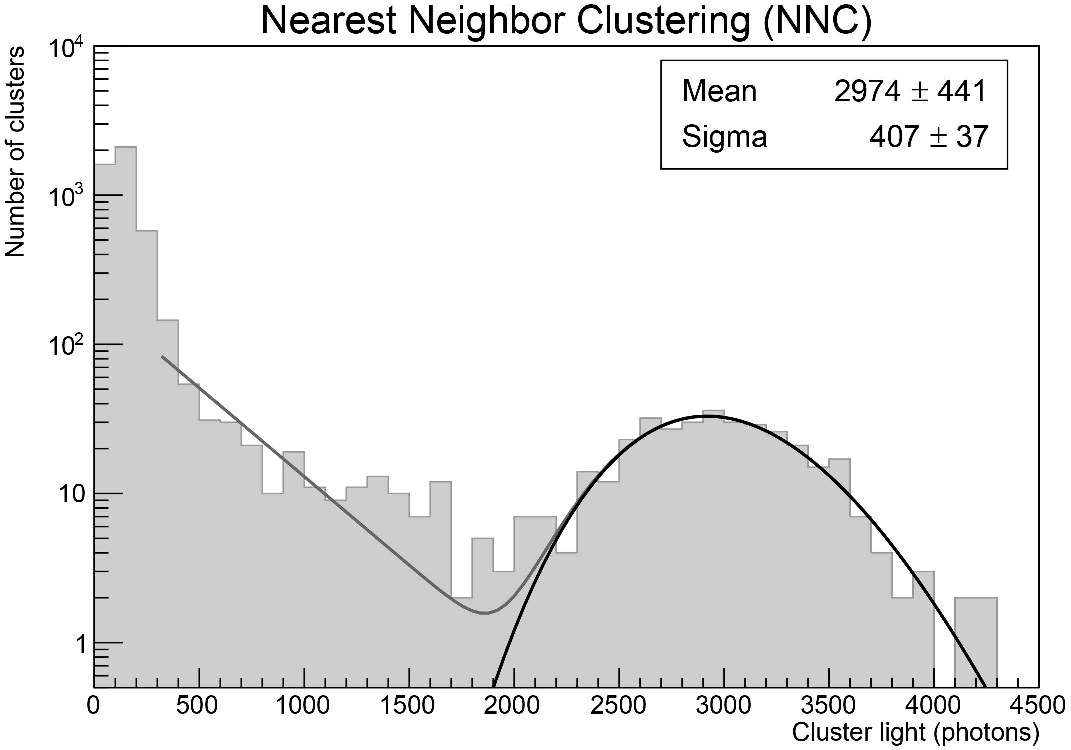
\includegraphics[width=0.44\textwidth]{log_Resolution_NNC_4.pdf}
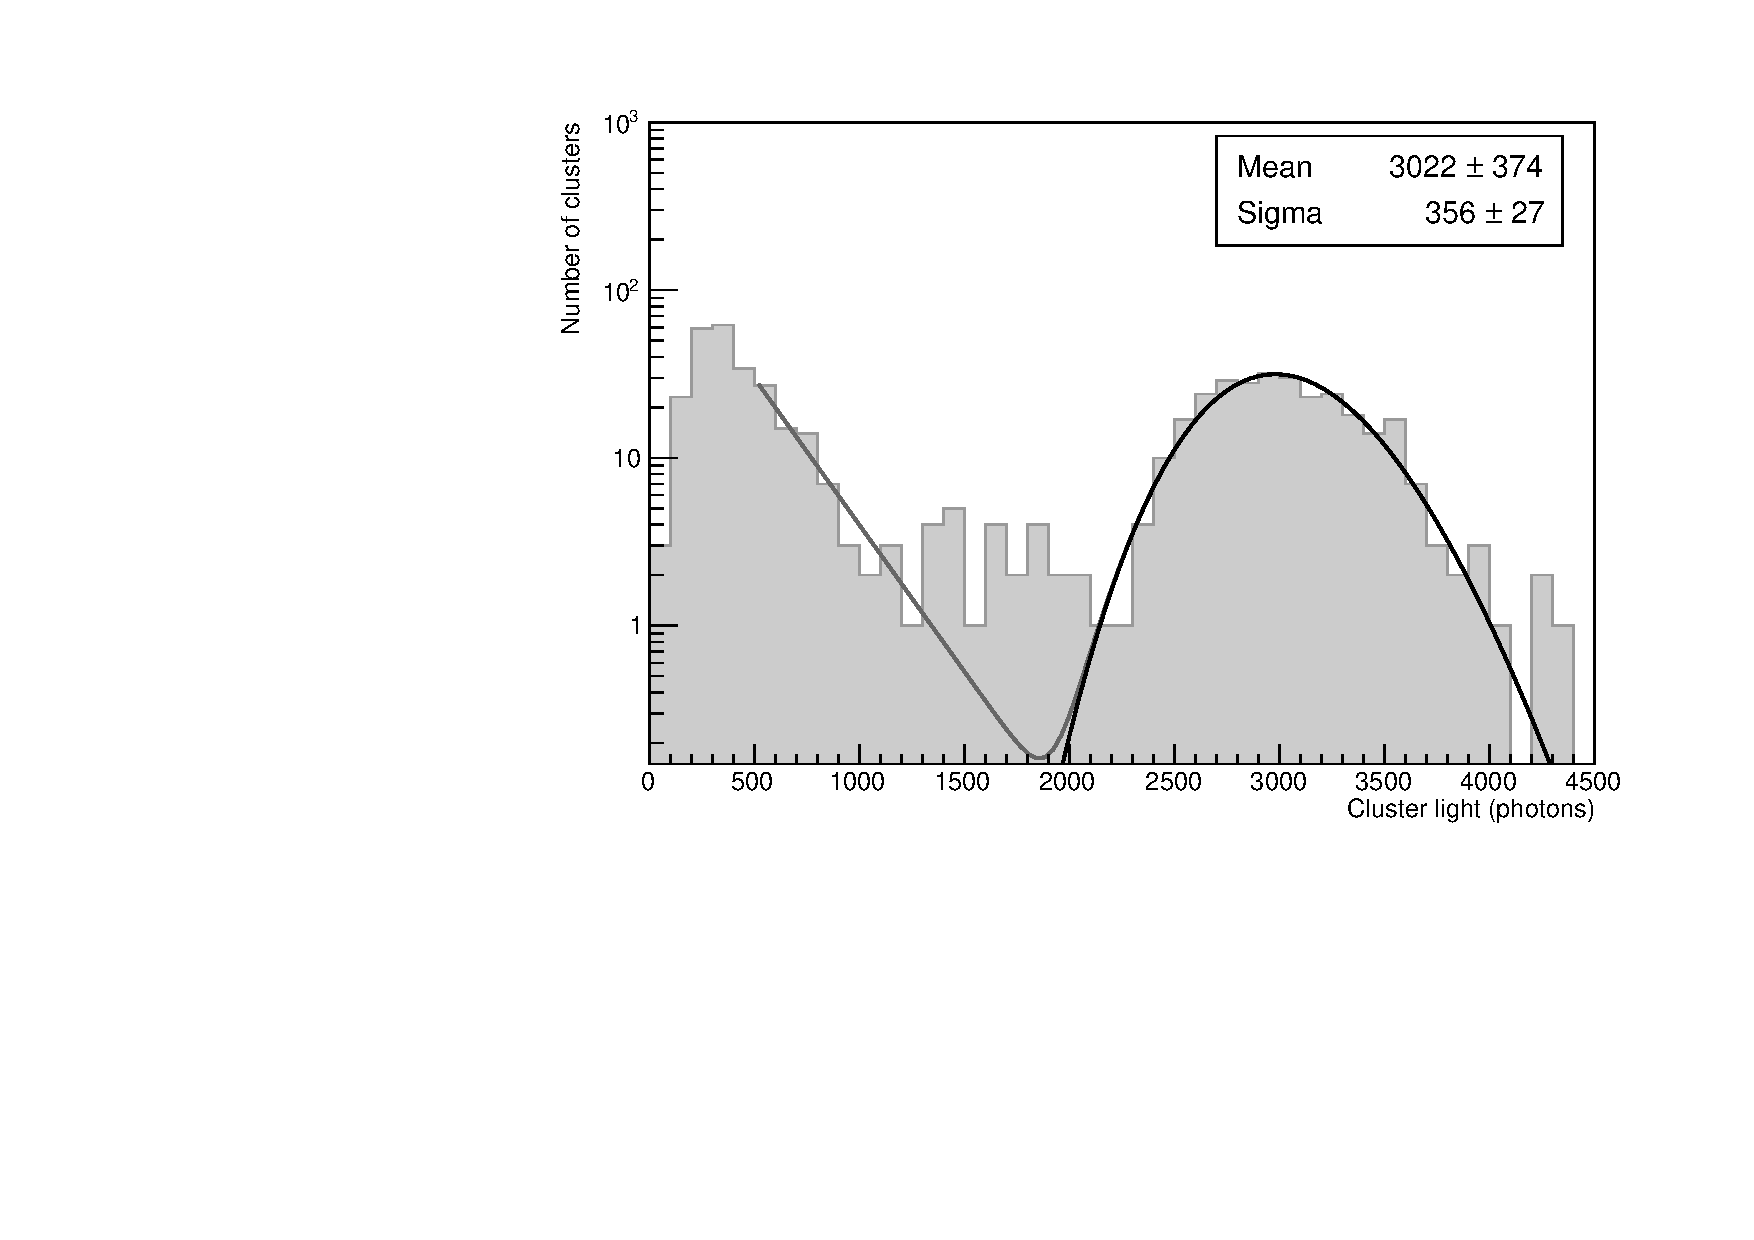
\includegraphics[width=0.44\textwidth]{log_Resolution_DB_4.pdf}
\caption{Results of the fit applied to the NNC (left) and iDBSCAN (right) energy distributions for clusters with slimness higher than 0.4.} 
\label{fig_CosFe_slim}
\end{figure}




% Please add the following required packages to your document preamble:
% \usepackage{multirow}
\begin{table}[ht]
\centering
\caption{Detector resolution comparison between NNC and iDBSCAN as a function of slimness.}
\label{tab:ResComp}
\begin{tabular}{c|cccc}
\multirow{2}{*}{\begin{tabular}[c]{@{}c@{}}Slimness\\ (width/lenght)\end{tabular}} & \multicolumn{4}{c}{Resolution (\%)}                                \\
                                                                                   & \multicolumn{2}{c|}{iDBSCAN}             & \multicolumn{2}{c}{NNC} \\ \hline \hline
0.0                                                                                & 12.2 & \multicolumn{1}{c|}{$\pm$ 1.8} & 18.1    & $\pm$ 3.9    \\
0.2                                                                                & 12.0 & \multicolumn{1}{c|}{$\pm$ 1.7} & 17.3    & $\pm$ 3.7    \\
0.4                                                                                & 11.8 & \multicolumn{1}{c|}{$\pm$ 1.7} & 13.7    & $\pm$ 2.4    \\
0.6                                                                                & 12.0 & \multicolumn{1}{c|}{$\pm$ 2.0} & 11.8    & $\pm$ 1.8    \\
0.8                                                                                & 12.3 & \multicolumn{1}{c|}{$\pm$ 3.8} & 11.1    & $\pm$ 2.8   
\end{tabular}
\end{table}


%\hfill \break

\newpage

\section{Summary}\label{sec:conclusion}

An adapted version of DBSCAN, named intensity-based DBSCAN, has recently been developed and tested on data acquired with a CYGNO TPC prototype. The impact of this algorithm on the detector performance has been studied using 5.9~keV photons from a $^{55}$Fe radioactive source and compared with results obtained with a simple NNC approach.
The iDBSCAN parameters were optimized for the running conditions of LEMOn, which uses a 4M pixels sCMOS camera, and for signals from $^{55}$Fe photons.
The obtained results showed that, with iDBSCAN, the clustering process of the CYGNO's event-reconstruction algorithm can achieve, without any other event-selection routine, a natural radioactivity background rejection in the energy region around 5.9~keV (from 3.0 keV to 8.8 keV) of 0.82$^{+0.04}_{-0.04}$ and a number of electronic-noise clusters per image of $(9 \pm 4)\times 10^{-4}$, occurring predominantly in the region below 1 keV ($\approx$ 500 photons).
Compared with NNC, these results represent an enhancement of 57\% for the former and, for the latter, an improvement by a factor of a few thousand. 
Finally, the detector energy resolution using iDBSCAN was measured to be (12.2 $\pm$ 1.8)\% for 5.9 keV electron recoil events. By requiring spots with slimness larger than 0.4, a rate of electronic-noise clusters per image of $(5 \pm 3)\times 10^{-4}$, a natural radioactive background rejection of 0.92$^{+0.03}_{-0.04}$ and an energy resolution of (11.8 $\pm$ 1.7)\% were achieved.

\acknowledgments
This work was supported by the European Research Council (ERC) under the European Union’s Horizon 2020 research and innovation program (grant agreement No 818744) and also by the Coordenação de Aperfeiçoamento de Pessoal de Nível Superior - Brasil (CAPES) - Finance Code 001.


\bibliographystyle{JHEP}
\bibliography{LEMON-20-002}


\end{document}
